\documentclass[serif,10pt]{beamer}

\def\gridopacity{100}
\def\gridopacity{0}

\usepackage{multimedia}

% see http://tex.stackexchange.com/a/24491
% for how to use enumitem with beamer
\usepackage{enumitem}
\setitemize{label=\usebeamerfont*{itemize item}%
  \usebeamercolor[fg]{itemize item}
  \usebeamertemplate{itemize item}}

% default page size is:
% \beamer@paperwidth 12.80cm%
% \beamer@paperheight 9.60cm%

\setbeamersize{text margin left=0.4cm,text margin right=0.4cm}

\usepackage{tikz}
\usetikzlibrary{calc,decorations.pathreplacing,fadings,positioning}
\usepackage{pgfplots}
\usepackage{pgfplotstable}

\tikzfading[name=fade down, bottom color=transparent!0, top color=transparent!100]

\usepackage{tikzvid}

\usepackage[clock,misc]{ifsym} % for \showclock

% pretty tables
\usepackage{multirow}
\usepackage{booktabs}

% this is from http://tex.stackexchange.com/a/103691
% taken from manual
\makeatletter
\pgfdeclareshape{document}{
\inheritsavedanchors[from=rectangle] % this is nearly a rectangle
\inheritanchorborder[from=rectangle]
\inheritanchor[from=rectangle]{center}
\inheritanchor[from=rectangle]{north}
\inheritanchor[from=rectangle]{south}
\inheritanchor[from=rectangle]{west}
\inheritanchor[from=rectangle]{east}
% ... and possibly more
\backgroundpath{% this is new
% store lower right in xa/ya and upper right in xb/yb
\southwest \pgf@xa=\pgf@x \pgf@ya=\pgf@y
\northeast \pgf@xb=\pgf@x \pgf@yb=\pgf@y
% compute corner of ‘‘flipped page’’
\pgf@xc=\pgf@xb \advance\pgf@xc by-10pt % this should be a parameter
\pgf@yc=\pgf@yb \advance\pgf@yc by-10pt
% construct main path
\pgfpathmoveto{\pgfpoint{\pgf@xa}{\pgf@ya}}
\pgfpathlineto{\pgfpoint{\pgf@xa}{\pgf@yb}}
\pgfpathlineto{\pgfpoint{\pgf@xc}{\pgf@yb}}
\pgfpathlineto{\pgfpoint{\pgf@xb}{\pgf@yc}}
\pgfpathlineto{\pgfpoint{\pgf@xb}{\pgf@ya}}
\pgfpathclose
% add little corner
\pgfpathmoveto{\pgfpoint{\pgf@xc}{\pgf@yb}}
\pgfpathlineto{\pgfpoint{\pgf@xc}{\pgf@yc}}
\pgfpathlineto{\pgfpoint{\pgf@xb}{\pgf@yc}}
\pgfpathlineto{\pgfpoint{\pgf@xc}{\pgf@yc}}
}
}
\makeatother

\usepackage{algorithm}
\usepackage[noend]{algpseudocode}

% symbols
\usepackage{amsmath} % assumes amsmath package installed
\usepackage{amssymb} % for \square
% non-italicized math subscripts
\newcommand{\ms}[1]{\mbox{\scriptsize #1}}
% from http://tex.stackexchange.com/a/5255
\DeclareMathOperator*{\argmin}{arg\,min}
\DeclareMathOperator*{\argmax}{arg\,max}

% fonts
\renewcommand\rmdefault{pplx}
\renewcommand\mathfamilydefault{cmr}

\setbeamertemplate{navigation symbols}{}

\setbeamerfont{page number in head/foot}{size=\small}
%\setbeamertemplate{footline}[frame number]
\setbeamertemplate{footline}{%
   \raisebox{7pt}{\makebox[\paperwidth]{%
   \hfill\makebox[10pt]{\textcolor{gray}{%
   \small\insertframenumber\hspace{0.1in}}}}}}

% dont number title page
\addtocounter{framenumber}{-1}

\title{Completing Manipulation Tasks Efficiently\\in Complex Environments}
\author{Christopher M. Dellin}
\date{August 22, 2016}

\begin{document}

\begin{frame}[plain]
   %\begin{columns}
   %   \column{1.2\textwidth}
      \maketitle
   %\end{columns}
\end{frame}


\begin{frame}
   \frametitle{Thesis Outline}

   Four pieces:

   HOW TO OPTIMIZE (SHORTEST PATHS ON GRAPHS)

   WHAT TO OPTIMIZE (MOTION PLANNING)

   \begin{itemize}
      \item Lazy Pathfinding (Alg: LazySP)
      \item Dynamic Pathfinding (Alg: IBiD)
      \item Utility Maximization (Alg: LEMUR)
      \item Planning over Configuration Space Families
   \end{itemize}

\end{frame}


\begin{frame}
   \frametitle{Talk Outline}
   \begin{tikzpicture}[font=\small]
      \tikzset{>=latex} % arrow heads
      \draw[step=1,black!15,very thin,opacity=\gridopacity] (0,0) grid (12,8);

      \node[fill=blue!15,minimum width=11cm] at (6,7.5) {\strut What to Optimize?};

      \node[fill=black!3,minimum width=5cm,minimum height=3cm] (utility) at (3.25,5.6) {};
      \node[anchor=north] at (utility.north) {\strut Maximizing Utility};
      \node at (3.25,5.35) {\includegraphics[width=2.5cm]{build/pvx-utility-anytime}};

      \node[fill=black!3,minimum width=5cm,minimum height=3cm] (family) at (8.75,5.6) {};
      \node[anchor=north] at (family.north) {\strut Utility in C-Space Familes};
      \node at (8.75,5.4) {\includegraphics[width=3.0cm]{build/multiple-sets}};

      \node[fill=blue!15,minimum width=11cm] at (6,3.5) {\strut How to Optimize?};

      \node[fill=black!3,minimum width=5cm,minimum height=3cm] (lazysp) at (3.25,1.6) {};
      \node[anchor=north] at (lazysp.north) {\strut Lazy Pathfinding};
      \node[draw=black!30,fill=white,inner sep=5pt] at (3.25,1.4) {
         \includegraphics[width=3.8cm]{build/lazysp-icon}};

      \node[fill=black!3,minimum width=5cm,minimum height=3cm] (ibid) at (8.75,1.6) {};
      \node[anchor=north] at (ibid.north) {\strut Dynamic Pathfinding};
      \node[draw=black!30,inner sep=0pt] at (8.75,1.4) {
         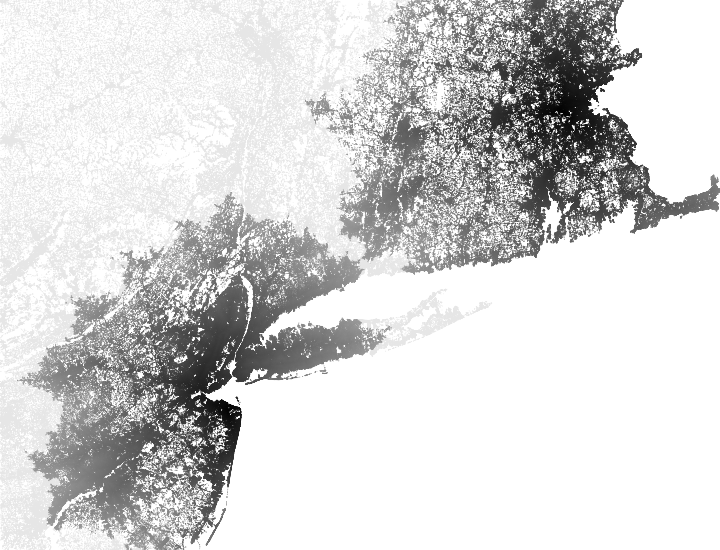
\includegraphics[width=2.9cm]{figs/incbi-road-ne/singleshot/example-bidijkstra.png}};

      \only<2>
      {
         \draw[ultra thick] (utility.north west) rectangle (utility.south east);
      }
      
   \end{tikzpicture}
\end{frame}

%\begin{frame}
%   \frametitle{Maximizing Utility in Motion Planning}
%   \begin{tikzpicture}[font=\small]
%      \tikzset{>=latex} % arrow heads
%
%      \draw[step=1,black!15,very thin,opacity=\gridopacity] (0,0) grid (12,8);
%
%      \node at ( 6,4) {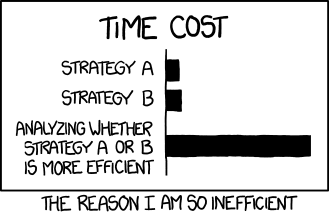
\includegraphics[width=5cm]{figs/xkcd-1445-efficiency.png}};
%      
%   \end{tikzpicture}
%\end{frame}

\begin{frame}
   \frametitle{Maximizing Utility in Motion Planning}
   \begin{tikzpicture}[font=\small]
      \tikzset{>=latex} % arrow heads

      \draw[step=1,black!15,very thin,opacity=\gridopacity] (0,0) grid (12,8);

      \node at (4,5) {\includegraphics{build/pvx-graph}};

      \node[fill=blue!5,align=center] at (9,5.5) {
         $A_1$, $A_2$: planner invocations\\
         $A_3$: a parameterized planner\\
         $A_4$: an anytime planner};

      \node[fill=blue!5,align=center] at (4.5,1.5) {
         $A$: an invocation of a motion planner\\
         $p$: planning cost incurred during invocation\\
         $x$: execution cost of resulting solution path\\
         $U(p,x)$: utility function which scores the invocation};

   \end{tikzpicture}
\end{frame}

\begin{frame}
   \frametitle{Examples of Utility Functions}
   \begin{tikzpicture}[font=\small]
      \tikzset{>=latex} % arrow heads
      \draw[step=1,black!15,very thin,opacity=\gridopacity] (0,0) grid (12,8);

      \node at (1.92,6.5) {\includegraphics{build/pvx-sm-firstfeas}};
      \node[anchor=west] at (3.5,6.5) {First Feasible};
      
      \node at (1.82,3.9) {\includegraphics{build/pvx-sm-xbudget}};
      \node[anchor=west] at (3.5,3.9) {Bounded Cost};
      
      \node at (1.92,1.3) {\includegraphics{build/pvx-sm-pbudget}};
      \node[anchor=west] at (3.5,1.3) {Planning Budget};

   \end{tikzpicture}
\end{frame}

\begin{frame}
   \frametitle{General Path Algorithm}
   \begin{tikzpicture}[font=\small]
      \tikzset{>=latex} % arrow heads
      \draw[step=1,black!15,very thin,opacity=\gridopacity] (0,0) grid (12,8);

      \node[fill=blue!5,rounded corners,anchor=north,minimum width=9.5cm,minimum height=3.3cm] (alg) at (6,7.75) {};
      \node[left=0.1cm of alg.north,anchor=north] {\begin{minipage}{9cm}
         \begin{algorithmic}[1]
         \For {iteration $i \in 1, 2, \dots$}
            \State $\bar{p}_i \leftarrow$
               planning cost incurred so far
            \State $\Xi_i \leftarrow$ set of paths to consider at iteration $i$
            \State $\grave{p}_i : \Xi_i \rightarrow \mathbb{R}^+$
               \Comment additional planning cost estimator
            \State $\hat{x}_i : \Xi_i \rightarrow \mathbb{R}^+$
               \Comment execution cost estimator
            \State $\xi_i = \argmax_{\xi \in \Xi_i}
               U\!\left( \; \bar{p}_i \! + \! \grave{p}_i(\xi), \; \hat{x}_i(\xi) \; \right)$
               \label{line:outline-argmax}
            \State \Return $\xi_i$
               if $\xi_i$ fully evaluated, i.e. $\grave{p}(\xi) = 0$
            \State evaluate $\xi_i$
               \Comment incurs requisite planning cost
         \EndFor
         \end{algorithmic}
      \end{minipage}};

      \only<1>{\node at (6.0,2.0) {\includegraphics{build/p-estimates}};}
      \only<2>{
      \node at (3.0,2.0) {\includegraphics{build/pvx-rrt}};
      \node at (9.0,2.0) {\includegraphics{build/rrt}};
      }

   \end{tikzpicture}
\end{frame}

\begin{frame}
   \frametitle{Maximizing Utility on Roadmaps}
   \begin{tikzpicture}[font=\small]
      \draw[step=1,black!15,very thin,opacity=\gridopacity] (0,0) grid (12,8);

      %\node[fill=blue!15,minimum width=11cm] at (6,7.5) {\strut How to Optimize?};
      %\node[fill=blue!15,minimum width=11cm] at (6,6.75) {\strut What to Optimize?};

      \node[fill=blue!5,rounded corners,anchor=north,minimum width=9.5cm,minimum height=3.3cm] (alg) at (6,7.75) {};
      \only<2->{
         \node[fill=blue!20,below=0.83cm of alg.north,minimum width=9.5cm,minimum height=0.4cm] {};
      }
      \node[left=0.1cm of alg.north,anchor=north] {\begin{minipage}{9cm}
         \begin{algorithmic}[1]
         \For {iteration $i \in 1, 2, \dots$}
            \State $\bar{p}_i \leftarrow$
               planning cost incurred so far
            \State $\Xi_i \leftarrow$ set of paths to consider at iteration $i$
            \State $\grave{p}_i : \Xi_i \rightarrow \mathbb{R}^+$
               \Comment additional planning cost estimator
            \State $\hat{x}_i : \Xi_i \rightarrow \mathbb{R}^+$
               \Comment execution cost estimator
            \State $\xi_i = \argmax_{\xi \in \Xi_i}
               U\!\left( \; \bar{p}_i \! + \! \grave{p}_i(\xi), \; \hat{x}_i(\xi) \; \right)$
               \label{line:outline-argmax}
            \State \Return $\xi_i$
               if $\xi_i$ fully evaluated, i.e. $\grave{p}(\xi) = 0$
            \State evaluate $\xi_i$
               \Comment incurs requisite planning cost
         \EndFor
         \end{algorithmic}
      \end{minipage}};

      \only<3->{
         \fill[white,path fading=fade down] (1,6.5) rectangle (11,6.0);
         \fill[white] (1,6.0) rectangle (11,4);

         \node at (2.25,3.25) {\includegraphics[width=3.0cm]{build/roadmap-stack-onramps}};

         \node[anchor=north,fill=black!3,rounded corners] at (8,5.5) {\begin{minipage}{7cm}
            \raggedright
         
            Focus: Roadmap methods

            \medskip
            Advantages:
            \begin{itemize}
            \item Well-studied asymptotic completeness\\
               and optimality properties
            \item Easy to progressively densify
            \item Common structure across queries\\
               (can load roadmaps from disk)
            \end{itemize}
         \end{minipage}};
      }
      
   \end{tikzpicture}
\end{frame}

\begin{frame}
   \frametitle{Maximizing Linear Utilities over Additive Estimators}
   \begin{tikzpicture}[font=\small]
      \draw[step=1,black!15,very thin,opacity=\gridopacity] (0,0) grid (12,8);
      \tikzset{>=latex} % arrow heads

      %\node[fill=blue!15,minimum width=11cm] at (6,7.5) {\strut How to Optimize?};
      %\node[fill=blue!15,minimum width=11cm] at (6,6.75) {\strut What to Optimize?};

      \node[fill=blue!5,rounded corners,anchor=north,minimum width=9.5cm,minimum height=3.3cm] (alg) at (6,7.75) {};
      \only<2->{
         \node[fill=blue!20,below=1.99cm of alg.north,minimum width=9.5cm,minimum height=0.43cm] {};
      }
      \node[left=0.1cm of alg.north,anchor=north] {\begin{minipage}{9cm}
         \begin{algorithmic}[1]
         \For {iteration $i \in 1, 2, \dots$}
            \State $\bar{p}_i \leftarrow$
               planning cost incurred so far
            \State $\Xi_i \leftarrow$ set of paths to consider at iteration $i$
            \State $\grave{p}_i : \Xi_i \rightarrow \mathbb{R}^+$
               \Comment additional planning cost estimator
            \State $\hat{x}_i : \Xi_i \rightarrow \mathbb{R}^+$
               \Comment execution cost estimator
            \State $\xi_i = \argmax_{\xi \in \Xi_i}
               U\!\left( \; \bar{p}_i \! + \! \grave{p}_i(\xi), \; \hat{x}_i(\xi) \; \right)$
               \label{line:outline-argmax}
            \State \Return $\xi_i$
               if $\xi_i$ fully evaluated, i.e. $\grave{p}(\xi) = 0$
            \State evaluate $\xi_i$
               \Comment incurs requisite planning cost
         \EndFor
         \end{algorithmic}
      \end{minipage}};

      \only<3->{
         \node[fill=black!3,rounded corners] at (3.0,3.0) {\begin{minipage}{4.9cm}
            We consider \emph{linear utility functions}:
            \vspace{-0.2cm}
            \[
               -U(p,x) = \lambda_U \, p + (1 - \lambda_U) \, x
            \]
         \end{minipage}};
      }
      \only<5->{
         \node[fill=black!3,rounded corners] at (8.7,3.0) {\begin{minipage}{5.6cm}
            We consider \emph{additive estimators}:
            \vspace{-0.2cm}
            \[
               \xi: \mbox{path on a roadmap graph } G
            \]
            \vspace{-0.5cm}
            \[
               \grave{p}_i(\xi) = \sum_{e \in \xi} \grave{p}_i(e)
               \;\;\mbox{and}\;\;
               \hat{x}_i(\xi) = \sum_{e \in \xi} \hat{x}_i(e)
            \]
         \end{minipage}};
      }

      \only<4>{
         %\node at (9.06,2.25) {\includegraphics[width=3.75cm]{build/pvx-linear-discounting}};
         \node at (8.5,2.25) {\includegraphics[width=3.75cm]{build/pvx-linear-discounting}};
      }

      \only<6->{
         \draw[->,very thick] (5.65,1.9) -- (5.65,1.4);
      
         \node[fill=black!3,rounded corners] at (5.8,0.8) {\begin{minipage}{5cm}
            Shortest path problem with:
            \vspace{-0.2cm}
            \[
               w_i(e) = \lambda_U \, \grave{p}_i(e) + (1 - \lambda_U) \, \hat{x}_i(e)
            \]
         \end{minipage}};
      }
      
   \end{tikzpicture}
\end{frame}

% all this data cumulative over the multistep-prescribed problem

\pgfplotstableread{
lambda searchmean evalmean
lam00 0.13717146918 1.566855428440001
lam20 0.13591121493999997 1.5040972085999997
lam50 0.12633906594 1.3774433666
lam80 0.11458146473999997 1.2423356615
lam99 0.10054155609999996 0.9362152972200001
}{\datasvetimeherbbinnom}

\pgfplotstableread{
lambda searchmean evalmean
lam00 0.9183584741400002 4.73433351068
lam20 0.8734410922000001 4.4884742077799995
lam50 0.82153580024 4.091855509880002
lam80 0.75752757384 3.39455290978
lam99 0.7430251334600001 3.0377397256199994
}{\datasvetimeworkcell}

\begin{frame}
   \frametitle{Search vs. Evaluation Planning Time Comparison}
   \begin{tikzpicture}[font=\small]
      \draw[step=1,black!15,very thin,opacity=\gridopacity] (0,0) grid (12,8);
      \tikzset{>=latex} % arrow heads

      \node at (8.2,7.5) {
         \protect\tikz{\protect\node[fill=red!20,draw=black]{};}\;graph search vs.
         \protect\tikz{\protect\node[fill=blue!20,draw=black]{};}\;edge evaluation
      };

      \node at ( 2.5,5.7) {
         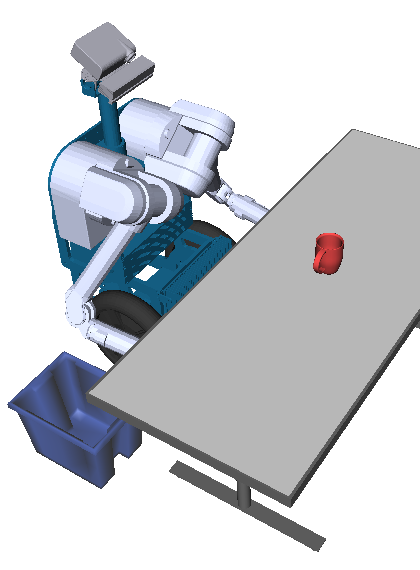
\includegraphics[width=1.7cm]{figs/herbbin/step0cropped.png}
         \;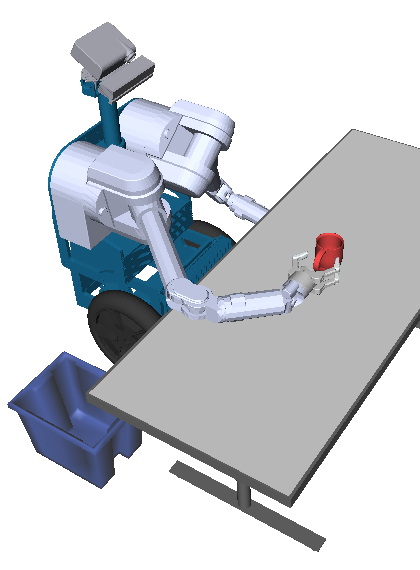
\includegraphics[width=1.7cm]{figs/herbbin/step01cropped.png}};

      \begin{scope}[shift={(5.5,5.0)}]
      \begin{axis}[
         width=7.0cm,
         height=3.2cm,
         xbar stacked,
         bar width=7,
         %xmin=0,xmax=10,
         xmin=0,
         %xtick pos=bottom,
         %symbolic y coords={E, F, R, A, B, W, P},
         %yticklabels from table={\datasvetimeherbbinnom}{lambda},
         yticklabels={$0.00$,,,,$0.99$},
         ylabel={$\lambda$},
         ytick=data,
         %ytick pos=left,
         xmajorgrids,
         xmajorticks=true,
         %ticklabel style={font=\footnotesize},
         enlarge y limits={abs=0.2cm},
         ylabel near ticks,
         ylabel shift=-0.5cm,
         ylabel style={rotate=-90},
         xlabel={Average S/E Planning Time (s)},
         xlabel near ticks,
         ] 
      %\node[circle,fill=white,inner sep=1pt,text=black!40] at (axis cs:40,-5.6) {\scriptsize 40};
      %\node[circle,fill=white,inner sep=1pt,text=black!40] at (axis cs:60,-5.6) {\scriptsize 60};
      %\node[circle,fill=white,inner sep=1pt,text=black!40] at (axis cs:80,-5.6) {\scriptsize 80};
      \addplot[color=black,fill=red!20]
         table[y expr=-\coordindex,x=searchmean]
         {\datasvetimeherbbinnom};
      \addplot[color=black,fill=blue!20]
         table[y expr=-\coordindex,x=evalmean]
         {\datasvetimeherbbinnom};
      \end{axis}
      \end{scope}

      \node at ( 2.5,2.2) {
         \includegraphics[width=3.5cm]{videos/workcell-cropped.png}};

      \begin{scope}[shift={(5.5,1.5)}]
      \begin{axis}[
         width=7.0cm,
         height=3.2cm,
         xbar stacked,
         bar width=7,
         %xmin=0,xmax=10,
         xmin=0,
         %xtick pos=bottom,
         %symbolic y coords={E, F, R, A, B, W, P},
         %yticklabels from table={\datasvetimeherbbinnom}{lambda},
         yticklabels={$0.00$,,,,$0.99$},
         ylabel={$\lambda$},
         ytick=data,
         %ytick pos=left,
         xmajorgrids,
         xmajorticks=true,
         %ticklabel style={font=\footnotesize},
         enlarge y limits={abs=0.2cm},
         ylabel near ticks,
         ylabel shift=-0.5cm,
         ylabel style={rotate=-90},
         xlabel={Average S/E Planning Time (s)},
         xlabel near ticks,
         ] 
      %\node[circle,fill=white,inner sep=1pt,text=black!40] at (axis cs:40,-5.6) {\scriptsize 40};
      %\node[circle,fill=white,inner sep=1pt,text=black!40] at (axis cs:60,-5.6) {\scriptsize 60};
      %\node[circle,fill=white,inner sep=1pt,text=black!40] at (axis cs:80,-5.6) {\scriptsize 80};
      \addplot[color=black,fill=red!20]
         table[y expr=-\coordindex,x=searchmean]
         {\datasvetimeworkcell};
      \addplot[color=black,fill=blue!20]
         table[y expr=-\coordindex,x=evalmean]
         {\datasvetimeworkcell};
      \end{axis}
      \end{scope}

   \end{tikzpicture}
\end{frame}


\begin{frame}
   \frametitle{Talk Outline}
   \begin{tikzpicture}[font=\small]
   \tikzset{>=latex} % arrow heads
   \draw[step=1,black!15,very thin,opacity=\gridopacity] (0,0) grid (12,8);

   % START LEMUR
   \node[fill=blue!5,draw=blue!10,rounded corners,minimum width=9.7cm,minimum height=5.8cm,anchor=north] (lemur) at (6,6.0) {};
   \node[anchor=north west] at (lemur.north west) {Planner};

   % left side
   \only<3->{
      \node[fill=blue!10,draw=blue!20,rounded corners,align=center,minimum height=1.5cm,minimum width=2.5cm,inner sep=0pt] at (3.3,4.5) {};
      \node at (3.3,4.5) {\includegraphics[width=1.8cm]{build/roadmap-stack-short}};
      \draw[->] (3.3,3.75) -- (3.3,3.0) node [pos=0.45,fill=blue!5,align=center,inner sep=2pt] {$G$};
   }

   % right side
   \only<5->{
   \node[fill=blue!10,draw=blue!20,rounded corners,align=center,minimum height=1.5cm,inner sep=0pt] at (7.8,4.5) {
         \qquad\qquad\; $ \arraycolsep=1.5pt \begin{array}{rcc}
            w_{\ms{est}}(e) = & \lambda \, \grave{p}(e) \; + & (1\!-\!\lambda) \, \hat{x}(e) \\
            w(e) = & & (1\!-\!\lambda) \, x(e)
         \end{array} $
      };
      %\node[fill=black!3,draw=blue!20,inner sep=2pt] at (7,5.4) {\includegraphics[width=1.3cm]{build/pvx-utility-anytime-simple}};
      \node[fill=black!3,draw=blue!20,inner sep=2pt] at (5.6,4.5) {\includegraphics[width=1.0cm]{build/pvx-linear-discounting-simple}};

      \draw[->] (7.3,3.75) -- (7.3,3.0) node [pos=0.45,fill=blue!5,align=center,inner sep=2pt] {$w$};
      \draw[->] (8.2,3.75) -- (8.2,3.0) node [pos=0.45,fill=blue!5,align=center,inner sep=2pt] {$w_{\ms{est}}$};
   }
   
   % START LAZYSP
   \node[fill=blue!10,draw=blue!20,rounded corners,minimum width=7cm,minimum height=2.5cm,anchor=north] (lazysp) at (6,3.0) {};
   \node[align=center] at (4,2.4) {Lazy\\Pathfinding};

   \node[draw=black!30,fill=white,inner sep=5pt] at (4,1.4) {
      \includegraphics[width=2.0cm]{build/lazysp-icon}};

   \node[fill=blue!20,draw=blue!30,rounded corners,align=center,minimum width=3.3cm,minimum height=2.1cm,anchor=north] (dynsp) at (7.5,2.8) {};
   \node[anchor=north west] at (dynsp.north west) {\begin{minipage}{3.1cm}Dynamic Pathfinding\end{minipage}};
   \node[draw=black!30,inner sep=0pt] at (7.5,1.55) {
      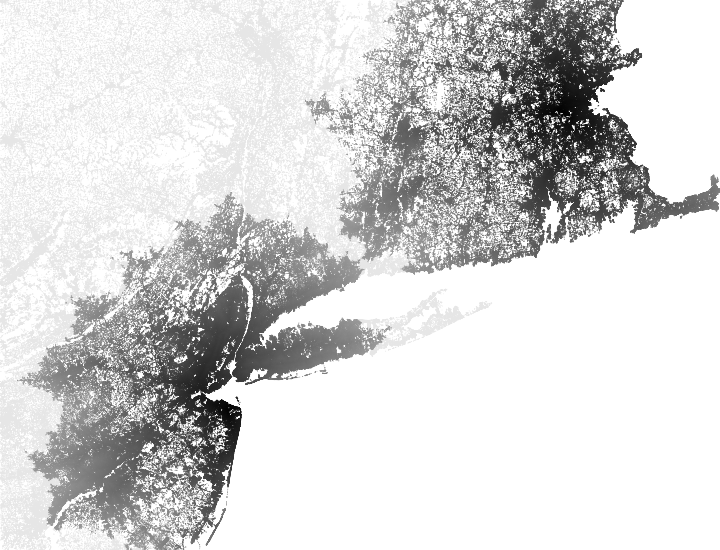
\includegraphics[width=2.0cm]{figs/incbi-road-ne/singleshot/example-bidijkstra.png}};

   % END LAZYSP

   % END LEMUR

   % top left side
   \only<2->{
      \node[fill=blue!10,draw=blue!20,rounded corners,align=center,minimum height=1.5cm,minimum width=1.8cm,inner sep=0pt] at (3.3,7.0) {};
      \node[fill=white,inner sep=0pt] at (3.3,7.0) {\includegraphics[width=1.4cm]{build/c-space-simple}};
      \node[font=\scriptsize] at (2.95,6.7) {$\mathcal{C}_{\mbox{\tiny free}}$};
   }
   \only<3->{
      \draw[->] (3.3,6.25) -- (3.3,5.25) node [pos=0.55,fill=blue!5,align=center,inner sep=0pt] {\strut $\mathcal{C}$};
   }

   %\node[inner sep=4pt] (cspace) at (3.3,7.0) {$\mathcal{C}$-Space};
   %\draw[->] (cspace) -- (3.3,5.25);
   
   % top right side
   \only<4->{
      \node[fill=blue!10,draw=blue!20,rounded corners,align=center,minimum height=1.5cm] at (7.9,7)
      {$\arraycolsep=1.5pt \begin{array}{cl}
         x(\xi)\!: & \mbox{execution cost} \;(\mathcal{C}_{\ms{free}}) \\
         \hat{x}(\xi)\!: & \mbox{execution cost estimate} \\
         \grave{p}(\xi)\!: & \mbox{planning cost estimate}
      \end{array}$};
   }

   \only<5->{
      \draw[->] (7.3,6.25) -- (7.3,5.25) node [pos=0.55,fill=blue!5,align=center,inner sep=0pt] {\strut $x$};
      \draw[->] (7.9,6.25) -- (7.9,5.25) node [pos=0.55,fill=blue!5,align=center,inner sep=0pt] {\strut $\hat{x}$};
      \draw[->] (8.5,6.25) -- (8.5,5.25) node [pos=0.55,fill=blue!5,align=center,inner sep=0pt] {\strut $\grave{p}$};
   }

   % left side
   \draw[->] (0.5,2.0) -- (2.5,2.0);
   \node[fill=white,align=center,inner sep=2pt] at (0.5,2.0)
      {$q_{\ms{start}}$\\$q_{\ms{dest}}$};

   % right side
   \draw[->] (9.5,2.0) -- (11.3,2.0);
   \node[fill=white,align=center,inner sep=2pt] at (11.5,2.0)
      {$\xi$};

   \only<6->{
      \draw[thick,rounded corners] (lazysp.south west) rectangle (lazysp.north east);
   }

   \end{tikzpicture}
\end{frame}

%\begin{frame}
%   \frametitle{Pathfinding on Graphs}
%   
%   The \emph{shortest-path problem} is prevalent and fundamental.
%   
%   Lots of applications.
%   
%   Graph $G=(V,E)$, edge weight function $w: E \rightarrow \mathbb{R}$.
%   
%   Single-pair, all-pairs, single-source/single-sink, etc.
%   
%   Bounded-suboptimal, incremental, anytime, etc ...
%\end{frame}

%\iffalse

\begin{frame}
   \frametitle{Motivation: The Shortest Path (SP) Problem}
   \begin{tikzpicture}[font=\small]
      \tikzset{>=latex} % arrow heads
   
      \draw[step=1,black!15,very thin,opacity=\gridopacity] (0,0) grid (12,8);
      
      \only<2->{
         \node at (1,7) {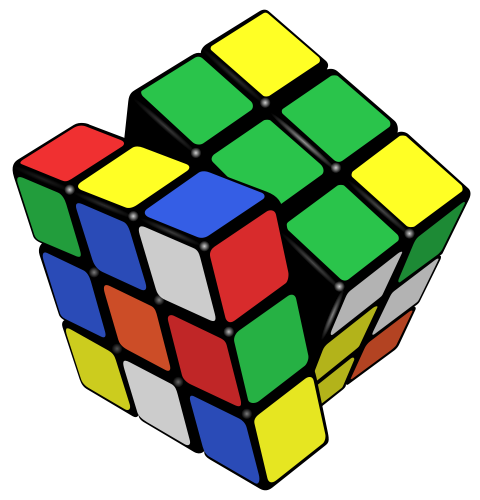
\includegraphics[width=1.5cm]{figs/rubik.png}};
         \node at (3,7) {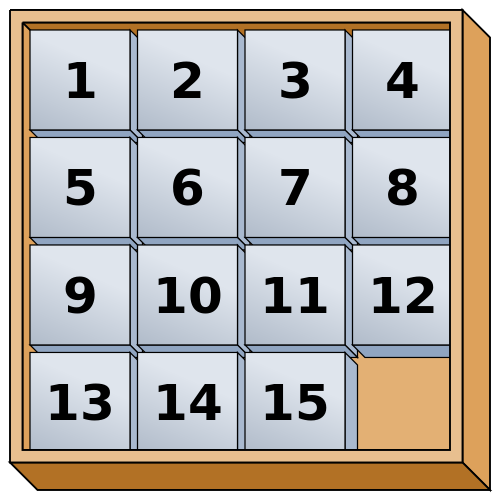
\includegraphics[width=1.5cm]{figs/15puzzle.png}};
      }
      \only<3->{
         \node at (5,7) {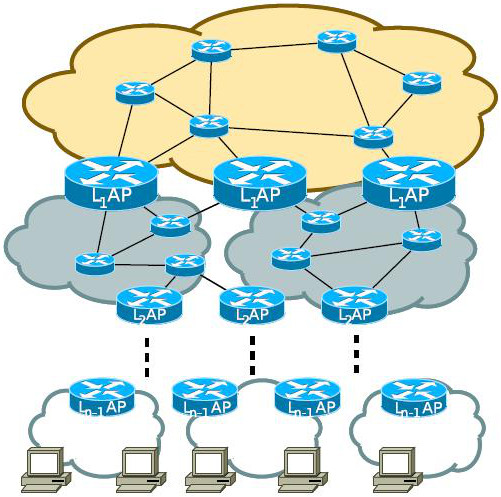
\includegraphics[width=1.5cm]{figs/internet-routers.jpg}};
      }
      \only<4->{
         \node at (7,7) {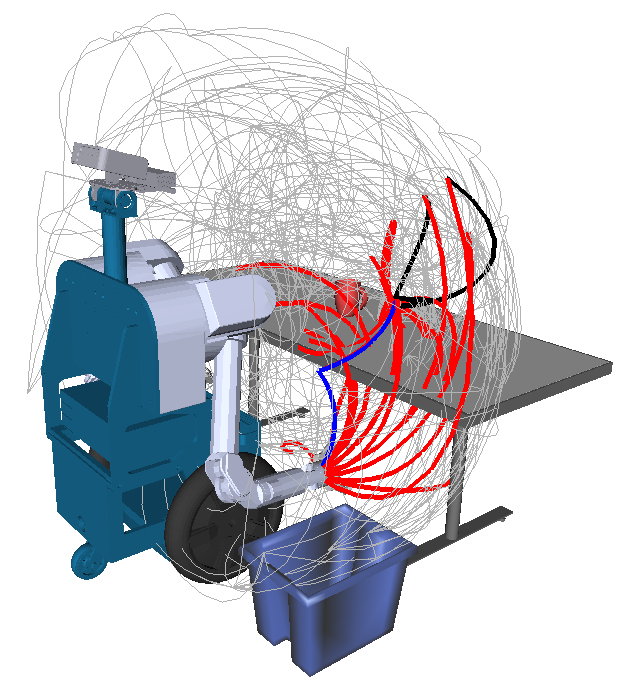
\includegraphics[width=1.5cm]{figs/lazysp-herbarm/herbarm-path33.png}};
         \node at (9,7) {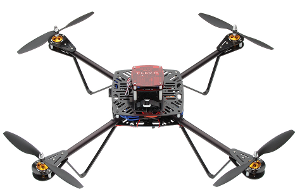
\includegraphics[width=1.5cm]{figs/quad.png}};
      }
      \only<5->{
         \node at (11,7) {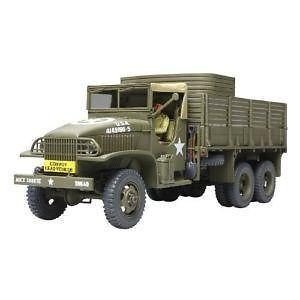
\includegraphics[width=1.5cm]{figs/military-truck.jpg}};
      }
      
      \only<6->{
         % graph
         
         \coordinate (va) at ( 2.0,4.0);
         \coordinate (vb) at ( 3.5,4.7);
         \coordinate (vc) at ( 4.0,5.9);
         \coordinate (vd) at ( 5.5,4.5);
         \coordinate (ve) at ( 8.0,5.0);
         \coordinate (vf) at (10.0,4.0);
         \coordinate (vg) at ( 1.5,5.0);
         \coordinate (vh) at ( 4.0,3.5);
         \coordinate (vi) at ( 7.0,3.2);
         \coordinate (vj) at ( 6.5,5.5);
         \coordinate (vk) at ( 9.0,3.5);
         
         \only<9->{
            \node[circle,fill=black!20,inner sep=0.1cm] at (va) {};
            \node[circle,fill=black!20,inner sep=0.1cm] at (vf) {};
         }
         
         \only<10->{
            \draw[line width=0.2cm,color=black!30,line cap=round]
               (va) -- (vb) -- (vd) -- (ve) -- (vf);
         }
         
         \node[circle,fill=black,inner sep=0.05cm] at (va) {};
         \node[circle,fill=black,inner sep=0.05cm] at (vb) {};
         \node[circle,fill=black,inner sep=0.05cm] at (vc) {};
         \node[circle,fill=black,inner sep=0.05cm] at (vd) {};
         \node[circle,fill=black,inner sep=0.05cm] at (ve) {};
         \node[circle,fill=black,inner sep=0.05cm] at (vf) {};
         \node[circle,fill=black,inner sep=0.05cm] at (vg) {};
         \node[circle,fill=black,inner sep=0.05cm] at (vh) {};
         \node[circle,fill=black,inner sep=0.05cm] at (vi) {};
         \node[circle,fill=black,inner sep=0.05cm] at (vj) {};
         \node[circle,fill=black,inner sep=0.05cm] at (vk) {};
         
         \draw (va) -- (vb) coordinate [midway] (eab);
         \draw (vb) -- (vc) coordinate [midway] (ebc);
         \draw (vb) -- (vd) coordinate [midway] (ebd);
         \draw (vc) -- (vd) coordinate [midway] (ecd);
         \draw (vd) -- (ve) coordinate [midway] (ede);
         \draw (ve) -- (vf) coordinate [midway] (eef);
         \draw (va) -- (vg) coordinate [midway] (eag);
         \draw (vb) -- (vg) coordinate [midway] (ebg);
         \draw (va) -- (vh) coordinate [midway] (eah);
         \draw (vd) -- (vh) coordinate [midway] (edh);
         \draw (vb) -- (vh) coordinate [midway] (ebh);
         \draw (vd) -- (vi) coordinate [midway] (edi);
         \draw (ve) -- (vi) coordinate [midway] (eei);
         \draw (vc) -- (vj) coordinate [midway] (ecj);
         \draw (vd) -- (vj) coordinate [midway] (edj);
         \draw (ve) -- (vj) coordinate [midway] (eej);
         \draw (vf) -- (vk) coordinate [midway] (efk);
         \draw (vi) -- (vk) coordinate [midway] (eik);
         \draw (ve) -- (vk) coordinate [midway] (eek);
         
         \only<7->{
            \node[circle,inner sep=0.02cm,fill=white,opacity=0.9,font=\scriptsize] at (eab) {5};
            \node[circle,inner sep=0.02cm,fill=white,opacity=0.9,font=\scriptsize] at (ebc) {5};
            \node[circle,inner sep=0.02cm,fill=white,opacity=0.9,font=\scriptsize] at (ebd) {6};
            \node[circle,inner sep=0.02cm,fill=white,opacity=0.9,font=\scriptsize] at (ecd) {7};
            \node[circle,inner sep=0.02cm,fill=white,opacity=0.9,font=\scriptsize] at (ede) {9};
            \node[circle,inner sep=0.02cm,fill=white,opacity=0.9,font=\scriptsize] at (eef) {7};
            \node[circle,inner sep=0.02cm,fill=white,opacity=0.9,font=\scriptsize] at (eag) {3};
            \node[circle,inner sep=0.02cm,fill=white,opacity=0.9,font=\scriptsize] at (ebg) {6};
            \node[circle,inner sep=0.02cm,fill=white,opacity=0.9,font=\scriptsize] at (eah) {6};
            \node[circle,inner sep=0.02cm,fill=white,opacity=0.9,font=\scriptsize] at (edh) {7};
            \node[circle,inner sep=0.02cm,fill=white,opacity=0.9,font=\scriptsize] at (ebh) {5};
            \node[circle,inner sep=0.02cm,fill=white,opacity=0.9,font=\scriptsize] at (edi) {8};
            \node[circle,inner sep=0.02cm,fill=white,opacity=0.9,font=\scriptsize] at (eei) {8};
            \node[circle,inner sep=0.02cm,fill=white,opacity=0.9,font=\scriptsize] at (ecj) {8};
            \node[circle,inner sep=0.02cm,fill=white,opacity=0.9,font=\scriptsize] at (edj) {6};
            \node[circle,inner sep=0.02cm,fill=white,opacity=0.9,font=\scriptsize] at (eej) {4};
            \node[circle,inner sep=0.02cm,fill=white,opacity=0.9,font=\scriptsize] at (efk) {3};
            \node[circle,inner sep=0.02cm,fill=white,opacity=0.9,font=\scriptsize] at (eik) {6};
            \node[circle,inner sep=0.02cm,fill=white,opacity=0.9,font=\scriptsize] at (eek) {6};
         }
      }
      
      \only<6->{
         \node[draw,align=center,minimum height=1.0cm,minimum width=2.9cm,thick]
            at (4.0,2.05) {Graph\\$G=(V,E)$};
      }
      \only<7->{
         \node[draw,align=center,minimum height=1.0cm,minimum width=2.9cm,thick]
            at (8.0,2.05) {Weight Function\\$w:E \rightarrow \mathbb{R}$};
         %\node[align=center,color=black!50] at (10.75,2) {
         %   $w(e) \geq 0$\\
         %   $w(e) > 0$\\
         %   $w(e) \geq w_{\ms{est}}(e)$\\
         %};
      }
      \only<8->{
         \node[draw,align=center,minimum height=1.0cm,minimum width=4cm,thick]
            (alg) at (6,0.55) {Shortest Path\\Algorithm};
         \draw[->] (4.5,1.55) -- (4.5,1.05);
         \draw[->] (7.5,1.55) -- (7.5,1.05);
      }
      \only<9->{
         \node[draw,align=center,shape=document,minimum width=3.0cm,ultra thin]
            (query) at (2,0.55) {Query $v_s$, $v_t$\;\;};
         \draw[->] (query.east) -- (alg.west);
         \node[left=0.1cm of va] {$v_s$};
         \node[right=0.1cm of vf] {$v_t$};
      }
      \only<10->{
         \node[draw,align=center,shape=document,minimum width=2.0cm,ultra thin]
            (path) at (10,0.55) {Path $p^*$\;};
         \draw[->] (alg.east) -- (path.west);
      }
      
   \end{tikzpicture}
\end{frame}

% application     -> graph representation    -> algorithm      -> path -> application solution
% [ lots of them]    G=(V,E)                    [lots of them]
%                    w: e -> R
%                    root vertices (v_s, v_t)
%                    (vertex heuristic?)
%                    problem
%                    - single-pair
%                    - optimal
%                    - bounded-suboptimal
%                    - bounded-cost
 
%\begin{frame}
%   \frametitle{Pathfinding on Graphs 2}
%   \begin{tikzpicture}
%      \tikzset{>=latex} % arrow heads
%   
%      \draw[step=1,black!15,very thin,opacity=\gridopacity] (0,0) grid (12,8);
%      
%      \node at (1.5,7.5) {Applications};
%      
%      \node at (1.0,6.5) {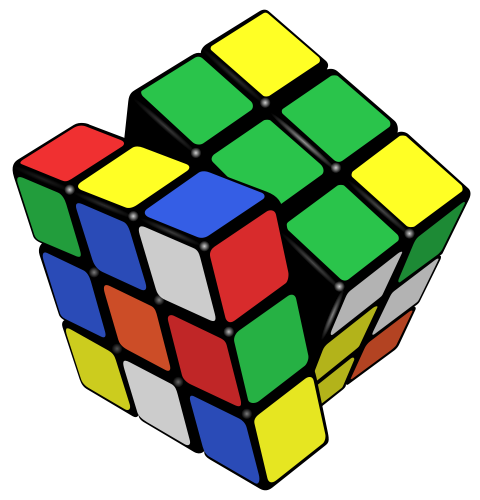
\includegraphics[width=1.5cm]{figs/rubik.png}};
%      \node at (2.0,6.5) {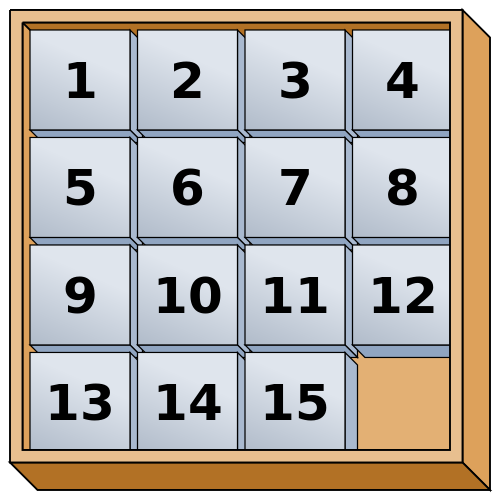
\includegraphics[width=1.5cm]{figs/15puzzle.png}};
%      \node at (1.5,4.5) {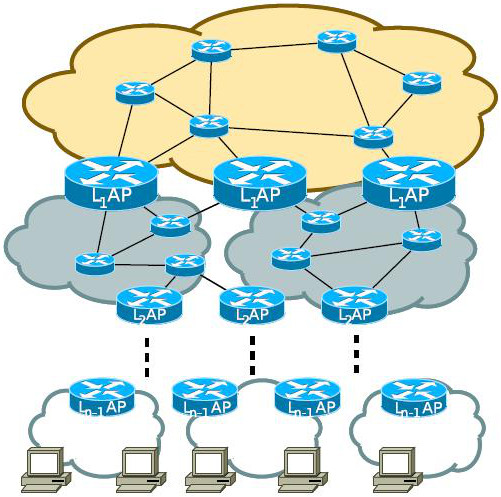
\includegraphics[width=1.5cm]{figs/internet-routers.jpg}};
%      \node at (1.5,3.0) {Traffic Routing};
%      \node at (1.5,2.5) {Motion Planning};
%      %\node at (1.5,2.0) {Optimal Motion Planning};
%      
%      \node at (6.0,7.5) {Representation};
%      
%      \node at (10.5,7.5) {Algorithms};
%      
%      \node[align=center] at (7,3) {
%         $w(e) \geq 0$\\
%         $w(e) > 0$\\
%         $w(e) \geq w_{\ms{est}}(e)$\\
%      };
%      
%      %\draw[step=1cm,black!10,very thin] (0,0) grid (8,4);
%      \node[draw,align=center,minimum height=1.0cm,thick]
%         at (6.0,6.0) {Graph\\$G=(V,E)$};
%      \node[draw,align=center,minimum height=1.0cm,thick]
%         at (6.0,4.5) {Weight Function\\$w:E \rightarrow [0,+\infty]$};
%      \node[draw,align=center,shape=document,minimum width=3.0cm,ultra thin]
%         (query) at (6,1) {Query $v_s$, $v_t$\;\;};
%      
%      \node at (10.5,6.5) {Dijkstra's};
%      \node at (10.5,5.5) {A*};
%      \node at (10.5,4.5) {IDA*};
%      \node at (10.5,3.5) {PEA*};
%      
%   \end{tikzpicture}
%\end{frame}

\begin{frame}
   \frametitle{Motivation: The Shortest Path (SP) Problem}
   \begin{tikzpicture}[font=\small]
      \tikzset{>=latex} % arrow heads
      
      \draw[step=1,black!15,very thin,opacity=\gridopacity] (0,0) grid (12,8);
   
      % c-space obstacles
      \only<8-12>{
         \fill[black!20] (4.5,3.25) rectangle (6.0,5.0);
         \fill[black!20] (8.5,4.00) rectangle (9.5,5.5);
         \only<8-10>{
            \node[color=black!70,font=\scriptsize] at (5.25,3.5) {$CO_1$};
            \node[color=black!70,font=\scriptsize] at (9.0,5.25) {$CO_2$};
         }
         \only<11->{
            \node[color=black!70,font=\scriptsize] at (5.25,3.5) {$SO_1$};
            \node[color=black!70,font=\scriptsize] at (9.0,5.25) {$SO_2$};
         }
      }
      
      % graph start
      \coordinate (va) at ( 2.0,4.0);
      \coordinate (vb) at ( 3.5,4.7);
      \coordinate (vc) at ( 4.0,5.9);
      \coordinate (vd) at ( 5.5,4.5);
      \coordinate (ve) at ( 8.0,5.0);
      \coordinate (vf) at (10.0,4.0);
      \coordinate (vg) at ( 1.5,5.0);
      \coordinate (vh) at ( 4.0,3.5);
      \coordinate (vi) at ( 7.0,3.2);
      \coordinate (vj) at ( 6.5,5.5);
      \coordinate (vk) at ( 9.0,3.5);
      
      %\node[circle,fill=black!20,inner sep=0.1cm] at (va) {};
      %\node[circle,fill=black!20,inner sep=0.1cm] at (vf) {};
      
      \node[circle,fill=black,inner sep=0.05cm] at (va) {};
      \node[circle,fill=black,inner sep=0.05cm] at (vb) {};
      \node[circle,fill=black,inner sep=0.05cm] at (vc) {};
      \node[circle,fill=black,inner sep=0.05cm] at (vd) {};
      \node[circle,fill=black,inner sep=0.05cm] at (ve) {};
      \node[circle,fill=black,inner sep=0.05cm] at (vf) {};
      \node[circle,fill=black,inner sep=0.05cm] at (vg) {};
      \node[circle,fill=black,inner sep=0.05cm] at (vh) {};
      \node[circle,fill=black,inner sep=0.05cm] at (vi) {};
      \node[circle,fill=black,inner sep=0.05cm] at (vj) {};
      \node[circle,fill=black,inner sep=0.05cm] at (vk) {};
      
      \draw (va) -- (vb) coordinate [midway] (eab);
      \draw (vb) -- (vc) coordinate [midway] (ebc);
      \draw (vb) -- (vd) coordinate [midway] (ebd);
      \draw (vc) -- (vd) coordinate [midway] (ecd);
      \draw (vd) -- (ve) coordinate [midway] (ede);
      \draw (ve) -- (vf) coordinate [midway] (eef);
      \draw (va) -- (vg) coordinate [midway] (eag);
      \draw (vb) -- (vg) coordinate [midway] (ebg);
      \draw (va) -- (vh) coordinate [midway] (eah);
      \draw (vd) -- (vh) coordinate [midway] (edh);
      \draw (vb) -- (vh) coordinate [midway] (ebh);
      \draw (vd) -- (vi) coordinate [midway] (edi);
      \draw (ve) -- (vi) coordinate [midway] (eei);
      \draw (vc) -- (vj) coordinate [midway] (ecj);
      \draw (vd) -- (vj) coordinate [midway] (edj);
      \draw (ve) -- (vj) coordinate [midway] (eej);
      \draw (vf) -- (vk) coordinate [midway] (efk);
      \draw (vi) -- (vk) coordinate [midway] (eik);
      \draw (ve) -- (vk) coordinate [midway] (eek);
      
      \only<4-4>{
         \node[circle,inner sep=0.02cm,fill=white,opacity=0.9,font=\scriptsize] at (eab) {1};
         \node[circle,inner sep=0.02cm,fill=white,opacity=0.9,font=\scriptsize] at (ebc) {1};
         \node[circle,inner sep=0.02cm,fill=white,opacity=0.9,font=\scriptsize] at (ebd) {1};
         \node[circle,inner sep=0.02cm,fill=white,opacity=0.9,font=\scriptsize] at (ecd) {1};
         \node[circle,inner sep=0.02cm,fill=white,opacity=0.9,font=\scriptsize] at (ede) {1};
         \node[circle,inner sep=0.02cm,fill=white,opacity=0.9,font=\scriptsize] at (eef) {1};
         \node[circle,inner sep=0.02cm,fill=white,opacity=0.9,font=\scriptsize] at (eag) {1};
         \node[circle,inner sep=0.02cm,fill=white,opacity=0.9,font=\scriptsize] at (ebg) {1};
         \node[circle,inner sep=0.02cm,fill=white,opacity=0.9,font=\scriptsize] at (eah) {1};
         \node[circle,inner sep=0.02cm,fill=white,opacity=0.9,font=\scriptsize] at (edh) {1};
         \node[circle,inner sep=0.02cm,fill=white,opacity=0.9,font=\scriptsize] at (ebh) {1};
         \node[circle,inner sep=0.02cm,fill=white,opacity=0.9,font=\scriptsize] at (edi) {1};
         \node[circle,inner sep=0.02cm,fill=white,opacity=0.9,font=\scriptsize] at (eei) {1};
         \node[circle,inner sep=0.02cm,fill=white,opacity=0.9,font=\scriptsize] at (ecj) {1};
         \node[circle,inner sep=0.02cm,fill=white,opacity=0.9,font=\scriptsize] at (edj) {1};
         \node[circle,inner sep=0.02cm,fill=white,opacity=0.9,font=\scriptsize] at (eej) {1};
         \node[circle,inner sep=0.02cm,fill=white,opacity=0.9,font=\scriptsize] at (efk) {1};
         \node[circle,inner sep=0.02cm,fill=white,opacity=0.9,font=\scriptsize] at (eik) {1};
         \node[circle,inner sep=0.02cm,fill=white,opacity=0.9,font=\scriptsize] at (eek) {1};
      }
      
      % motion planning
      \only<7-9>{
         \node[circle,inner sep=0.02cm,fill=white,opacity=0.9,font=\scriptsize] at (eab) {5};
         \node[circle,inner sep=0.02cm,fill=white,opacity=0.9,font=\scriptsize] at (ebc) {5};
         \node[circle,inner sep=0.02cm,fill=white,opacity=0.9,font=\scriptsize] at (ebd) {6};
         \node[circle,inner sep=0.02cm,fill=white,opacity=0.9,font=\scriptsize] at (ecd) {7};
         \node[circle,inner sep=0.02cm,fill=white,opacity=0.9,font=\scriptsize] at (ede) {9};
         \node[circle,inner sep=0.02cm,fill=white,opacity=0.9,font=\scriptsize] at (eef) {7};
         \node[circle,inner sep=0.02cm,fill=white,opacity=0.9,font=\scriptsize] at (eag) {3};
         \node[circle,inner sep=0.02cm,fill=white,opacity=0.9,font=\scriptsize] at (ebg) {6};
         \node[circle,inner sep=0.02cm,fill=white,opacity=0.9,font=\scriptsize] at (eah) {6};
         \node[circle,inner sep=0.02cm,fill=white,opacity=0.9,font=\scriptsize] at (edh) {7};
         \node[circle,inner sep=0.02cm,fill=white,opacity=0.9,font=\scriptsize] at (ebh) {5};
         \node[circle,inner sep=0.02cm,fill=white,opacity=0.9,font=\scriptsize] at (edi) {8};
         \node[circle,inner sep=0.02cm,fill=white,opacity=0.9,font=\scriptsize] at (eei) {8};
         \node[circle,inner sep=0.02cm,fill=white,opacity=0.9,font=\scriptsize] at (ecj) {8};
         \node[circle,inner sep=0.02cm,fill=white,opacity=0.9,font=\scriptsize] at (edj) {6};
         \node[circle,inner sep=0.02cm,fill=white,opacity=0.9,font=\scriptsize] at (eej) {4};
         \node[circle,inner sep=0.02cm,fill=white,opacity=0.9,font=\scriptsize] at (efk) {3};
         \node[circle,inner sep=0.02cm,fill=white,opacity=0.9,font=\scriptsize] at (eik) {6};
         \node[circle,inner sep=0.02cm,fill=white,opacity=0.9,font=\scriptsize] at (eek) {6};
      }
      \only<10-12>{
         \node[circle,inner sep=0.02cm,fill=white,opacity=0.9,font=\scriptsize] at (eab) {5};
         \node[circle,inner sep=0.02cm,fill=white,opacity=0.9,font=\scriptsize] at (ebc) {5};
         \node[circle,inner sep=0.02cm,fill=white,opacity=0.9,font=\scriptsize] at (ebd) {$\infty$};
         \node[circle,inner sep=0.02cm,fill=white,opacity=0.9,font=\scriptsize] at (ecd) {$\infty$};
         \node[circle,inner sep=0.02cm,fill=white,opacity=0.9,font=\scriptsize] at (ede) {$\infty$};
         \node[circle,inner sep=0.02cm,fill=white,opacity=0.9,font=\scriptsize] at (eef) {$\infty$};
         \node[circle,inner sep=0.02cm,fill=white,opacity=0.9,font=\scriptsize] at (eag) {3};
         \node[circle,inner sep=0.02cm,fill=white,opacity=0.9,font=\scriptsize] at (ebg) {6};
         \node[circle,inner sep=0.02cm,fill=white,opacity=0.9,font=\scriptsize] at (eah) {6};
         \node[circle,inner sep=0.02cm,fill=white,opacity=0.9,font=\scriptsize] at (edh) {$\infty$};
         \node[circle,inner sep=0.02cm,fill=white,opacity=0.9,font=\scriptsize] at (ebh) {5};
         \node[circle,inner sep=0.02cm,fill=white,opacity=0.9,font=\scriptsize] at (edi) {$\infty$};
         \node[circle,inner sep=0.02cm,fill=white,opacity=0.9,font=\scriptsize] at (eei) {8};
         \node[circle,inner sep=0.02cm,fill=white,opacity=0.9,font=\scriptsize] at (ecj) {8};
         \node[circle,inner sep=0.02cm,fill=white,opacity=0.9,font=\scriptsize] at (edj) {$\infty$};
         \node[circle,inner sep=0.02cm,fill=white,opacity=0.9,font=\scriptsize] at (eej) {4};
         \node[circle,inner sep=0.02cm,fill=white,opacity=0.9,font=\scriptsize] at (efk) {3};
         \node[circle,inner sep=0.02cm,fill=white,opacity=0.9,font=\scriptsize] at (eik) {6};
         \node[circle,inner sep=0.02cm,fill=white,opacity=0.9,font=\scriptsize] at (eek) {$\infty$};
      }
      
      % convoy
      \only<14->{
         \node[circle,inner sep=0.02cm,fill=white,opacity=0.9,font=\scriptsize] at (eab) {?};
         \node[circle,inner sep=0.02cm,fill=white,opacity=0.9,font=\scriptsize] at (ebc) {?};
         \node[circle,inner sep=0.02cm,fill=white,opacity=0.9,font=\scriptsize] at (ebd) {?};
         \node[circle,inner sep=0.02cm,fill=white,opacity=0.9,font=\scriptsize] at (ecd) {?};
         \node[circle,inner sep=0.02cm,fill=white,opacity=0.9,font=\scriptsize] at (ede) {?};
         \node[circle,inner sep=0.02cm,fill=white,opacity=0.9,font=\scriptsize] at (eef) {?};
         \node[circle,inner sep=0.02cm,fill=white,opacity=0.9,font=\scriptsize] at (eag) {?};
         \node[circle,inner sep=0.02cm,fill=white,opacity=0.9,font=\scriptsize] at (ebg) {?};
         \node[circle,inner sep=0.02cm,fill=white,opacity=0.9,font=\scriptsize] at (eah) {?};
         \node[circle,inner sep=0.02cm,fill=white,opacity=0.9,font=\scriptsize] at (edh) {?};
         \node[circle,inner sep=0.02cm,fill=white,opacity=0.9,font=\scriptsize] at (ebh) {?};
         %\node[circle,inner sep=0.02cm,fill=white,opacity=0.9,font=\scriptsize] at (edi) {?};
         \node[circle,inner sep=0.02cm,fill=white,opacity=0.9,font=\scriptsize] at (eei) {?};
         \node[circle,inner sep=0.02cm,fill=white,opacity=0.9,font=\scriptsize] at (ecj) {?};
         \node[circle,inner sep=0.02cm,fill=white,opacity=0.9,font=\scriptsize] at (edj) {?};
         \node[circle,inner sep=0.02cm,fill=white,opacity=0.9,font=\scriptsize] at (eej) {?};
         \node[circle,inner sep=0.02cm,fill=white,opacity=0.9,font=\scriptsize] at (efk) {?};
         \node[circle,inner sep=0.02cm,fill=white,opacity=0.9,font=\scriptsize] at (eik) {?};
         % first uncover
         \only<14-15>{\node[circle,inner sep=0.02cm,fill=white,opacity=0.9,font=\scriptsize] at (eek) {?};}
         \only<16->{  \node[circle,inner sep=0.02cm,fill=white,opacity=0.9,font=\scriptsize] (sateek) at (eek) {7.8};}
         \only<16>{\draw[ultra thick,red,->] (satnode.south west) -- (sateek.east);}
         % second uncover
         \only<14-16>{\node[circle,inner sep=0.02cm,fill=white,opacity=0.9,font=\scriptsize] at (edi) {?};}
         \only<17->{  \node[circle,inner sep=0.02cm,fill=white,opacity=0.9,font=\scriptsize] (satedi) at (edi) {$\infty$};}
         \only<17>{\draw[ultra thick,red,->] (satnode.south west) -- (satedi.east);}
      }

      %\node[left=0.1cm of va] {$v_s$};
      %\node[right=0.1cm of vf] {$v_t$};
      
      \only<9>{
         \draw (vb) -- (vd) node[pos=0.1,circle,fill=red,inner sep=0.05cm] {};
         \draw (vb) -- (vd) node[pos=0.2,circle,fill=red,inner sep=0.05cm] {};
         \draw (vb) -- (vd) node[pos=0.3,circle,fill=red,inner sep=0.05cm] {};
         \draw (vb) -- (vd) node[pos=0.4,circle,fill=red,inner sep=0.05cm] {};
         \draw (vb) -- (vd) node[pos=0.5,circle,fill=red,inner sep=0.05cm] {};
         \draw (vb) -- (vd) node[pos=0.6,circle,fill=red,inner sep=0.05cm] {};
         \draw (vb) -- (vd) node[pos=0.7,circle,fill=red,inner sep=0.05cm] {};
         \draw (vb) -- (vd) node[pos=0.8,circle,fill=red,inner sep=0.05cm] {};
         \draw (vb) -- (vd) node[pos=0.9,circle,fill=red,inner sep=0.05cm] {};
      }
      
      %\fill[white,opacity=0.8] (0,3) rectangle (12,6.5);
      % graph end
      
      \node[draw,thick,minimum height=1.5cm,minimum width=5.5cm,anchor=north] at (3,2.9) {};
      \node [anchor=north] at (3,2.9) {\begin{minipage}{5cm}
         \begin{center}
         Graph $G=(V,E)$:
         \end{center}
         \vspace{-0.3cm}
         
         % puzzles
         \only<3-4>{
            $v:$ puzzle state; $|V| = 10^{19}$
            
            $e:$ puzzle move
         }
         
         % highlight motion planning
         \only<6-10>{
            $v:$ arm configuration; $|V| \approx 10^{5}$
         
            $e:$ arm motion
         }
      \end{minipage}};
   
      \node[draw,thick,minimum height=1.5cm,minimum width=5.5cm,anchor=north] at (9,2.9) {};
      \node [anchor=north] at (9,2.9) {\begin{minipage}{5cm}
         \begin{center}
         Weight Function $w:E \rightarrow \mathbb{R}$:
         \end{center}
         \vspace{-0.3cm}
      
         % puzzles
         \only<4-4>{
            \vspace{0.2cm}
            $w(e) = 1 \; \forall e \in E$
         }
         
         % highlight motion planning
         \only<7-7>{%
            $w(e) = \left\{ \arraycolsep=2pt \begin{array}{cl}
            ||e|| & \mbox{if } e \in \mathcal{C}_{\ms{free}} \\
            & \\
            \end{array} \right.$
         }%
         \only<8-10>{%
            $w(e) = \left\{ \arraycolsep=2pt \begin{array}{cl}
            ||e|| & \mbox{if } e \in \mathcal{C}_{\ms{free}} \\
            \infty & \mbox{otherwise} \\
            \end{array} \right.$
         }%
         \only<12-12>{%
            \vspace{0.07cm}
            $w(e) = \mbox{BVP}(q_a, q_b)$
            
            {\footnotesize (solve a boundary-value problem)}
         }%
         \only<15->{%
            \vspace{0.2cm}
            $w(e) = \mbox{Reconnaissance}(e)$
         }%
      \end{minipage}};
   
      \node at (1,7) {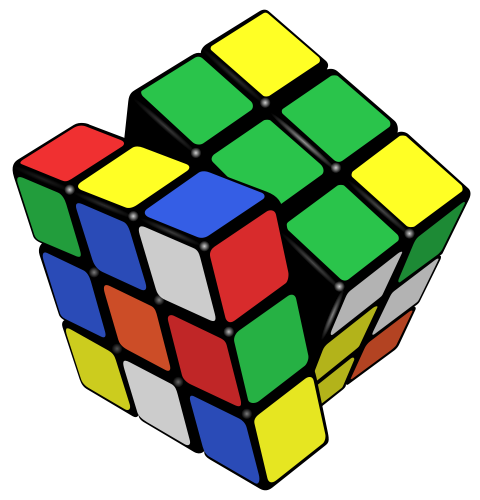
\includegraphics[width=1.5cm]{figs/rubik.png}};
      \node at (3,7) {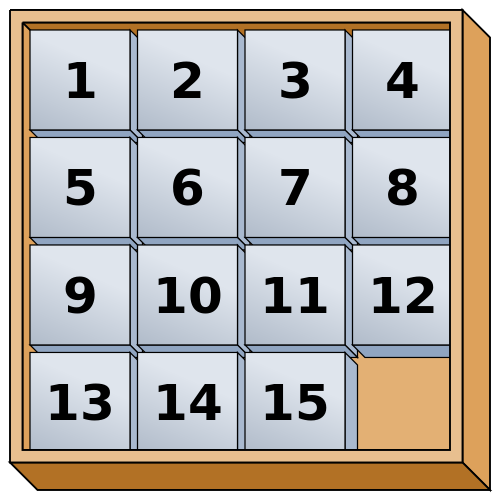
\includegraphics[width=1.5cm]{figs/15puzzle.png}};
      \node at (5,7) {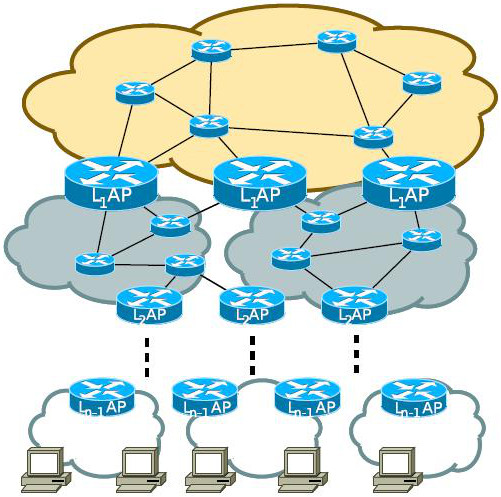
\includegraphics[width=1.5cm]{figs/internet-routers.jpg}};
      \node at (7,7) {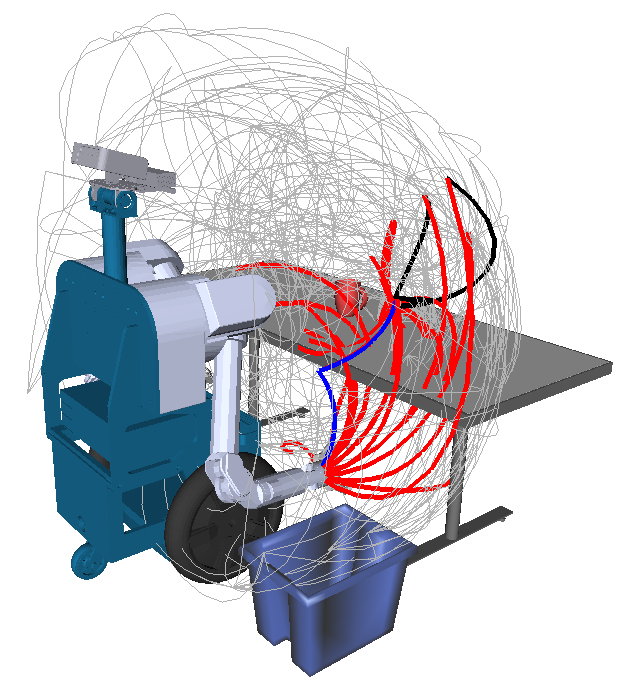
\includegraphics[width=1.5cm]{figs/lazysp-herbarm/herbarm-path33.png}};
      \node at (9,7) {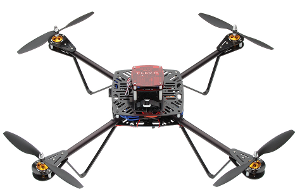
\includegraphics[width=1.5cm]{figs/quad.png}};
      \node at (11,7) {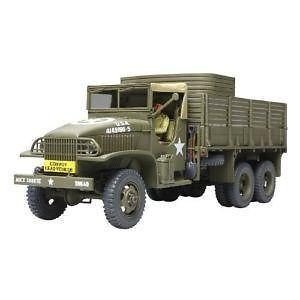
\includegraphics[width=1.5cm]{figs/military-truck.jpg}};
      
      % highlight nothing
      \only<1>{
         \fill[white,opacity=0.8] (0,6) rectangle (12,8);
      }
      
      % highlight puzzles
      \only<2-4>{
         \draw[ultra thick,rounded corners] (0.1,6.1) rectangle (3.9,7.9);
         \fill[white,opacity=0.8] (4,6) rectangle (12,8);
      }
      
      % highlight motion planning
      \only<5-10>{
         \draw[ultra thick,rounded corners] (6.1,6.1) rectangle (7.9,7.9);
         \fill[white,opacity=0.8] (0,6) rectangle (6,8);
         \fill[white,opacity=0.8] (8,6) rectangle (12,8);
         \only<6->{
            \node[align=center,font=\scriptsize] at (11.0,5.0) {Configuration\\Space};
         }
      }
      
      % highlight kinodynamic planning
      \only<11-12>{
         \draw[ultra thick,rounded corners] (8.1,6.1) rectangle (9.9,7.9);
         \fill[white,opacity=0.8] (0,6) rectangle (8,8);
         \fill[white,opacity=0.8] (10,6) rectangle (12,8);
         \node[align=center,font=\scriptsize] at (11.0,5.0) {Kinodynamic\\State Space};
      }
      
      % highlight convoy
      \only<13->{
         \draw[ultra thick,rounded corners] (10.1,6.1) rectangle (11.9,7.9);
         \fill[white,opacity=0.8] (0,6) rectangle (10,8);
         \only<15->{
            \node[draw,align=center,font=\scriptsize] (satnode) at (11.0,5.5) {Satellite};
         }
      }
      
      \node[draw,align=center,minimum height=1.0cm,minimum width=4cm,thick]
         (alg) at (6,0.55) {Shortest Path\\Algorithm};
      \draw[->] (4.5,1.40) -- (4.5,1.05);
      \draw[->] (7.5,1.40) -- (7.5,1.05);
      \node[draw,align=center,shape=document,minimum width=3.0cm,ultra thin]
         (query) at (2,0.55) {Query $v_s$, $v_t$\;\;};
      \draw[->] (query.east) -- (alg.west);
      \node[draw,align=center,shape=document,minimum width=2.0cm,ultra thin]
         (path) at (10,0.55) {Path $p^*$\;};
      \draw[->] (alg.east) -- (path.west);
   
   \end{tikzpicture}
\end{frame}






\begin{frame}
   \frametitle{Motivation: The Shortest Path (SP) Problem}
   \begin{tikzpicture}[font=\small]
      \tikzset{>=latex} % arrow heads
      \draw[step=1,black!15,very thin,opacity=\gridopacity] (0,0) grid (12,8);
      
      \node at (1,7) {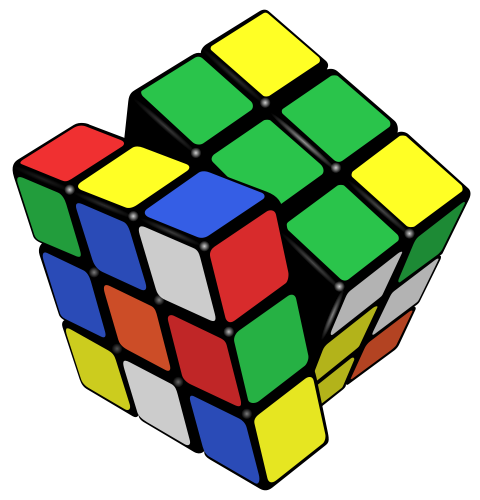
\includegraphics[width=1.5cm]{figs/rubik.png}};
      \node at (3,7) {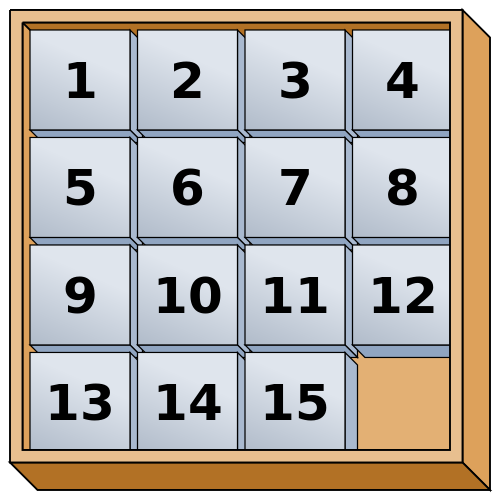
\includegraphics[width=1.5cm]{figs/15puzzle.png}};
      \node at (5,7) {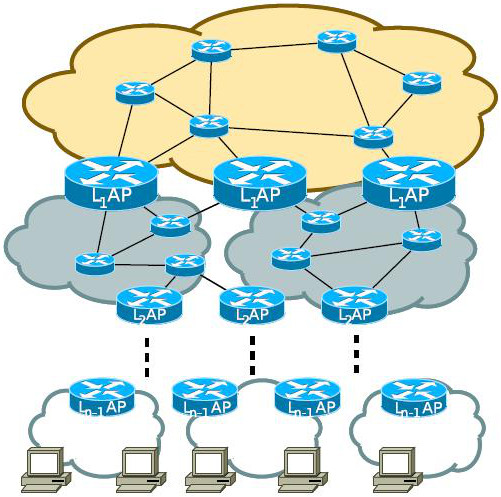
\includegraphics[width=1.5cm]{figs/internet-routers.jpg}};
      \node at (7,7) {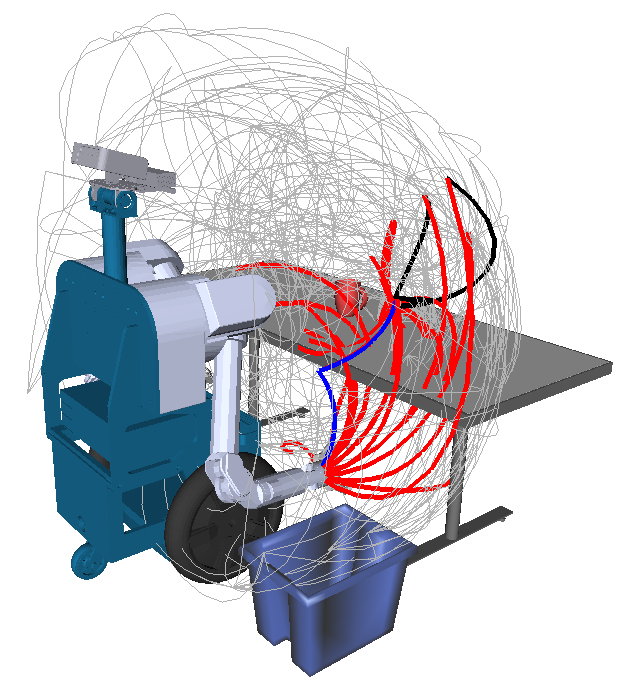
\includegraphics[width=1.5cm]{figs/lazysp-herbarm/herbarm-path33.png}};
      \node at (9,7) {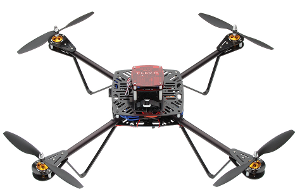
\includegraphics[width=1.5cm]{figs/quad.png}};
      \node at (11,7) {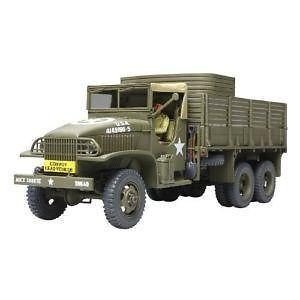
\includegraphics[width=1.5cm]{figs/military-truck.jpg}};
         
      \coordinate (va) at ( 2.0,4.0);
      \coordinate (vb) at ( 3.5,4.7);
      \coordinate (vc) at ( 4.0,5.9);
      \coordinate (vd) at ( 5.5,4.5);
      \coordinate (ve) at ( 8.0,5.0);
      \coordinate (vf) at (10.0,4.0);
      \coordinate (vg) at ( 1.5,5.0);
      \coordinate (vh) at ( 4.0,3.5);
      \coordinate (vi) at ( 7.0,3.2);
      \coordinate (vj) at ( 6.5,5.5);
      \coordinate (vk) at ( 9.0,3.5);

      \node[circle,fill=black!20,inner sep=0.1cm] at (va) {};
      \node[circle,fill=black!20,inner sep=0.1cm] at (vf) {};

      \draw[line width=0.2cm,color=black!30,line cap=round]
         (va) -- (vb) -- (vd) -- (ve) -- (vf);

      \node[circle,fill=black,inner sep=0.05cm] at (va) {};
      \node[circle,fill=black,inner sep=0.05cm] at (vb) {};
      \node[circle,fill=black,inner sep=0.05cm] at (vc) {};
      \node[circle,fill=black,inner sep=0.05cm] at (vd) {};
      \node[circle,fill=black,inner sep=0.05cm] at (ve) {};
      \node[circle,fill=black,inner sep=0.05cm] at (vf) {};
      \node[circle,fill=black,inner sep=0.05cm] at (vg) {};
      \node[circle,fill=black,inner sep=0.05cm] at (vh) {};
      \node[circle,fill=black,inner sep=0.05cm] at (vi) {};
      \node[circle,fill=black,inner sep=0.05cm] at (vj) {};
      \node[circle,fill=black,inner sep=0.05cm] at (vk) {};
      
      \draw (va) -- (vb) coordinate [midway] (eab);
      \draw (vb) -- (vc) coordinate [midway] (ebc);
      \draw (vb) -- (vd) coordinate [midway] (ebd);
      \draw (vc) -- (vd) coordinate [midway] (ecd);
      \draw (vd) -- (ve) coordinate [midway] (ede);
      \draw (ve) -- (vf) coordinate [midway] (eef);
      \draw (va) -- (vg) coordinate [midway] (eag);
      \draw (vb) -- (vg) coordinate [midway] (ebg);
      \draw (va) -- (vh) coordinate [midway] (eah);
      \draw (vd) -- (vh) coordinate [midway] (edh);
      \draw (vb) -- (vh) coordinate [midway] (ebh);
      \draw (vd) -- (vi) coordinate [midway] (edi);
      \draw (ve) -- (vi) coordinate [midway] (eei);
      \draw (vc) -- (vj) coordinate [midway] (ecj);
      \draw (vd) -- (vj) coordinate [midway] (edj);
      \draw (ve) -- (vj) coordinate [midway] (eej);
      \draw (vf) -- (vk) coordinate [midway] (efk);
      \draw (vi) -- (vk) coordinate [midway] (eik);
      \draw (ve) -- (vk) coordinate [midway] (eek);
         
      \node[circle,inner sep=0.02cm,fill=white,opacity=0.9,font=\scriptsize] at (eab) {5};
      \node[circle,inner sep=0.02cm,fill=white,opacity=0.9,font=\scriptsize] at (ebc) {5};
      \node[circle,inner sep=0.02cm,fill=white,opacity=0.9,font=\scriptsize] at (ebd) {6};
      \node[circle,inner sep=0.02cm,fill=white,opacity=0.9,font=\scriptsize] at (ecd) {7};
      \node[circle,inner sep=0.02cm,fill=white,opacity=0.9,font=\scriptsize] at (ede) {9};
      \node[circle,inner sep=0.02cm,fill=white,opacity=0.9,font=\scriptsize] at (eef) {7};
      \node[circle,inner sep=0.02cm,fill=white,opacity=0.9,font=\scriptsize] at (eag) {3};
      \node[circle,inner sep=0.02cm,fill=white,opacity=0.9,font=\scriptsize] at (ebg) {6};
      \node[circle,inner sep=0.02cm,fill=white,opacity=0.9,font=\scriptsize] at (eah) {6};
      \node[circle,inner sep=0.02cm,fill=white,opacity=0.9,font=\scriptsize] at (edh) {7};
      \node[circle,inner sep=0.02cm,fill=white,opacity=0.9,font=\scriptsize] at (ebh) {5};
      \node[circle,inner sep=0.02cm,fill=white,opacity=0.9,font=\scriptsize] at (edi) {8};
      \node[circle,inner sep=0.02cm,fill=white,opacity=0.9,font=\scriptsize] at (eei) {8};
      \node[circle,inner sep=0.02cm,fill=white,opacity=0.9,font=\scriptsize] at (ecj) {8};
      \node[circle,inner sep=0.02cm,fill=white,opacity=0.9,font=\scriptsize] at (edj) {6};
      \node[circle,inner sep=0.02cm,fill=white,opacity=0.9,font=\scriptsize] at (eej) {4};
      \node[circle,inner sep=0.02cm,fill=white,opacity=0.9,font=\scriptsize] at (efk) {3};
      \node[circle,inner sep=0.02cm,fill=white,opacity=0.9,font=\scriptsize] at (eik) {6};
      \node[circle,inner sep=0.02cm,fill=white,opacity=0.9,font=\scriptsize] at (eek) {6};

      %\node[draw,align=center,minimum height=1.0cm,minimum width=2.9cm,thick]
         %at (4.0,2.05) {Graph\\$G=(V,E)$};

      %\node[draw,align=center,minimum height=1.0cm,minimum width=2.9cm,thick]
         %at (8.0,2.05) {Weight Function\\$w:E \rightarrow \mathbb{R}$};

      %\node[draw,align=center,minimum height=1.0cm,minimum width=4cm,thick]
         %(alg) at (6,0.55) {Shortest Path\\Algorithm};
      %\draw[->] (4.5,1.55) -- (4.5,1.05);
      %\draw[->] (7.5,1.55) -- (7.5,1.05);

      %\node[draw,align=center,shape=document,minimum width=3.0cm,ultra thin]
         %(query) at (2,0.55) {Query $v_s$, $v_t$\;\;};
      %\draw[->] (query.east) -- (alg.west);
      %\node[left=0.1cm of va] {$v_s$};
      %\node[right=0.1cm of vf] {$v_t$};
      
      %\node[draw,align=center,shape=document,minimum width=2.0cm,ultra thin]
         %(path) at (10,0.55) {Path $p^*$\;};
      %\draw[->] (alg.east) -- (path.west);

      \node[fill=blue!15,rounded corners,font=\small] at (6,1.75)
      {\begin{minipage}{8cm}

         In some domains, determining edge weights\\
         is a computationally expensive operation.

         \vspace{0.1cm}
         \large
         \emph{Q: How can we solve shortest-path problems\\
         while reducing the number of edges evaluated?}

      \end{minipage}};
      
   \end{tikzpicture}
\end{frame}


%\begin{frame}
   %\frametitle{Pathfinding with Expensive Edge Evaluations}
   
   %In some domains, determining edge weights\\
   %is a computationally expensive operation.
   
   %\pause
   %\vspace{0.4cm}
   %\emph{Question: How can we solve shortest-path problems\\
      %\quad \quad \quad \quad \, while reducing the number of edges evaluated?}
   
   %\pause
   %\vspace{0.4cm}
   %Outline:
   %\begin{itemize}
   %\pause
   %\item Review of lazy search approaches
   %\pause
   %\item LazySP algorithm outline (using \emph{edge selectors})
   %\pause
   %\item Equivalence to existing algorithms
   %\pause
   %\item Novel edge selectors
   %%\pause
   %%\item Experimental results
   %\end{itemize}
%\end{frame}

\begin{frame}
   \frametitle{Review of Prior Approaches}
   
   \begin{tikzpicture}[font=\small]
      \tikzset{>=latex} % arrow heads
      
      \draw[step=1,black!15,very thin,opacity=\gridopacity] (0,0) grid (12,8);
      
      % graph start
      \coordinate (va) at ( 2.0,5.6);
      \coordinate (vb) at ( 3.5,6.3);
      \coordinate (vc) at ( 4.0,7.5);
      \coordinate (vd) at ( 5.5,6.1);
      \coordinate (ve) at ( 8.0,6.6);
      \coordinate (vf) at (10.0,5.6);
      \coordinate (vg) at ( 1.5,6.6);
      \coordinate (vh) at ( 4.0,5.1);
      \coordinate (vi) at ( 7.0,4.8);
      \coordinate (vj) at ( 6.5,7.1);
      \coordinate (vk) at ( 9.0,5.1);
      
      % start/goal highlighting
      \node[circle,fill=black!20,inner sep=0.1cm] at (va) {};
      \node[circle,fill=black!20,inner sep=0.1cm] at (vf) {};
      
      % edges, grey
      \only<1-2,4,10>{
         \draw[black!30] (va) -- (vb) coordinate [midway] (eab);
         \draw[black!30] (vb) -- (vc) coordinate [midway] (ebc);
         \draw[black!30] (vb) -- (vd) coordinate [midway] (ebd);
         \draw[black!30] (vc) -- (vd) coordinate [midway] (ecd);
         \draw[black!30] (vd) -- (ve) coordinate [midway] (ede);
         \draw[black!30] (ve) -- (vf) coordinate [midway] (eef);
         \draw[black!30] (va) -- (vg) coordinate [midway] (eag);
         \draw[black!30] (vb) -- (vg) coordinate [midway] (ebg);
         \draw[black!30] (va) -- (vh) coordinate [midway] (eah);
         \draw[black!30] (vd) -- (vh) coordinate [midway] (edh);
         \draw[black!30] (vb) -- (vh) coordinate [midway] (ebh);
         \draw[black!30] (vd) -- (vi) coordinate [midway] (edi);
         \draw[black!30] (ve) -- (vi) coordinate [midway] (eei);
         \draw[black!30] (vc) -- (vj) coordinate [midway] (ecj);
         \draw[black!30] (vd) -- (vj) coordinate [midway] (edj);
         \draw[black!30] (ve) -- (vj) coordinate [midway] (eej);
         \draw[black!30] (vf) -- (vk) coordinate [midway] (efk);
         \draw[black!30] (vi) -- (vk) coordinate [midway] (eik);
         \draw[black!30] (ve) -- (vk) coordinate [midway] (eek);
         
         \node[circle,inner sep=0.02cm,fill=white,opacity=0.9,font=\scriptsize] at (eab) {?};
         \node[circle,inner sep=0.02cm,fill=white,opacity=0.9,font=\scriptsize] at (ebc) {?};
         \node[circle,inner sep=0.02cm,fill=white,opacity=0.9,font=\scriptsize] at (ebd) {?};
         \node[circle,inner sep=0.02cm,fill=white,opacity=0.9,font=\scriptsize] at (ecd) {?};
         \node[circle,inner sep=0.02cm,fill=white,opacity=0.9,font=\scriptsize] at (ede) {?};
         \node[circle,inner sep=0.02cm,fill=white,opacity=0.9,font=\scriptsize] at (eef) {?};
         \node[circle,inner sep=0.02cm,fill=white,opacity=0.9,font=\scriptsize] at (eag) {?};
         \node[circle,inner sep=0.02cm,fill=white,opacity=0.9,font=\scriptsize] at (ebg) {?};
         \node[circle,inner sep=0.02cm,fill=white,opacity=0.9,font=\scriptsize] at (eah) {?};
         \node[circle,inner sep=0.02cm,fill=white,opacity=0.9,font=\scriptsize] at (edh) {?};
         \node[circle,inner sep=0.02cm,fill=white,opacity=0.9,font=\scriptsize] at (ebh) {?};
         \node[circle,inner sep=0.02cm,fill=white,opacity=0.9,font=\scriptsize] at (edi) {?};
         \node[circle,inner sep=0.02cm,fill=white,opacity=0.9,font=\scriptsize] at (eei) {?};
         \node[circle,inner sep=0.02cm,fill=white,opacity=0.9,font=\scriptsize] at (ecj) {?};
         \node[circle,inner sep=0.02cm,fill=white,opacity=0.9,font=\scriptsize] at (edj) {?};
         \node[circle,inner sep=0.02cm,fill=white,opacity=0.9,font=\scriptsize] at (eej) {?};
         \node[circle,inner sep=0.02cm,fill=white,opacity=0.9,font=\scriptsize] at (efk) {?};
         \node[circle,inner sep=0.02cm,fill=white,opacity=0.9,font=\scriptsize] at (eik) {?};
         \node[circle,inner sep=0.02cm,fill=white,opacity=0.9,font=\scriptsize] at (eek) {?};
      }
      
      % edges, black
      \only<3>{
         \draw[ultra thick] (va) -- (vb) coordinate [midway] (eab);
         \draw[ultra thick] (vb) -- (vc) coordinate [midway] (ebc);
         \draw[ultra thick] (vb) -- (vd) coordinate [midway] (ebd);
         \draw[ultra thick] (vc) -- (vd) coordinate [midway] (ecd);
         \draw[ultra thick] (vd) -- (ve) coordinate [midway] (ede);
         \draw[ultra thick] (ve) -- (vf) coordinate [midway] (eef);
         \draw[ultra thick] (va) -- (vg) coordinate [midway] (eag);
         \draw[ultra thick] (vb) -- (vg) coordinate [midway] (ebg);
         \draw[ultra thick] (va) -- (vh) coordinate [midway] (eah);
         \draw[ultra thick] (vd) -- (vh) coordinate [midway] (edh);
         \draw[ultra thick] (vb) -- (vh) coordinate [midway] (ebh);
         \draw[ultra thick] (vd) -- (vi) coordinate [midway] (edi);
         \draw[ultra thick] (ve) -- (vi) coordinate [midway] (eei);
         \draw[ultra thick] (vc) -- (vj) coordinate [midway] (ecj);
         \draw[ultra thick] (vd) -- (vj) coordinate [midway] (edj);
         \draw[ultra thick] (ve) -- (vj) coordinate [midway] (eej);
         \draw[ultra thick] (vf) -- (vk) coordinate [midway] (efk);
         \draw[ultra thick] (vi) -- (vk) coordinate [midway] (eik);
         \draw[ultra thick] (ve) -- (vk) coordinate [midway] (eek);
         
         \node[circle,inner sep=0.02cm,fill=white,opacity=0.9,font=\scriptsize] at (eab) {5};
         \node[circle,inner sep=0.02cm,fill=white,opacity=0.9,font=\scriptsize] at (ebc) {5};
         \node[circle,inner sep=0.02cm,fill=white,opacity=0.9,font=\scriptsize] at (ebd) {6};
         \node[circle,inner sep=0.02cm,fill=white,opacity=0.9,font=\scriptsize] at (ecd) {7};
         \node[circle,inner sep=0.02cm,fill=white,opacity=0.9,font=\scriptsize] at (ede) {9};
         \node[circle,inner sep=0.02cm,fill=white,opacity=0.9,font=\scriptsize] at (eef) {7};
         \node[circle,inner sep=0.02cm,fill=white,opacity=0.9,font=\scriptsize] at (eag) {3};
         \node[circle,inner sep=0.02cm,fill=white,opacity=0.9,font=\scriptsize] at (ebg) {6};
         \node[circle,inner sep=0.02cm,fill=white,opacity=0.9,font=\scriptsize] at (eah) {6};
         \node[circle,inner sep=0.02cm,fill=white,opacity=0.9,font=\scriptsize] at (edh) {7};
         \node[circle,inner sep=0.02cm,fill=white,opacity=0.9,font=\scriptsize] at (ebh) {5};
         \node[circle,inner sep=0.02cm,fill=white,opacity=0.9,font=\scriptsize] at (edi) {8};
         \node[circle,inner sep=0.02cm,fill=white,opacity=0.9,font=\scriptsize] at (eei) {8};
         \node[circle,inner sep=0.02cm,fill=white,opacity=0.9,font=\scriptsize] at (ecj) {8};
         \node[circle,inner sep=0.02cm,fill=white,opacity=0.9,font=\scriptsize] at (edj) {6};
         \node[circle,inner sep=0.02cm,fill=white,opacity=0.9,font=\scriptsize] at (eej) {4};
         \node[circle,inner sep=0.02cm,fill=white,opacity=0.9,font=\scriptsize] at (efk) {3};
         \node[circle,inner sep=0.02cm,fill=white,opacity=0.9,font=\scriptsize] at (eik) {6};
         \node[circle,inner sep=0.02cm,fill=white,opacity=0.9,font=\scriptsize] at (eek) {6};
      }
      
      % NEXT, A* stuff
      
      % OPEN list highlighting (A*)
      \only<5>{\node[circle,fill=blue!70,inner sep=0.15cm] at (va) {};}
      \only<6-9>{\node[circle,fill=black!40,inner sep=0.15cm] at (va) {};}
      \only<6>{\node[circle,fill=blue!70,inner sep=0.15cm] at (vb) {};}
      \only<7-9>{\node[circle,fill=black!40,inner sep=0.15cm] at (vb) {};}
      \only<6-9>{\node[circle,fill=blue!40,inner sep=0.15cm] at (vg) {};}
      \only<6>{\node[circle,fill=blue!40,inner sep=0.15cm] at (vh) {};}
      \only<7>{\node[circle,fill=blue!70,inner sep=0.15cm] at (vh) {};}
      \only<8-9>{\node[circle,fill=black!40,inner sep=0.15cm] at (vh) {};}
      \only<7>{\node[circle,fill=blue!40,inner sep=0.15cm] at (vc) {};}
      \only<8>{\node[circle,fill=blue!70,inner sep=0.15cm] at (vc) {};}
      \only<9>{\node[circle,fill=black!40,inner sep=0.15cm] at (vc) {};}
      \only<7-9>{\node[circle,fill=blue!40,inner sep=0.15cm] at (vd) {};}
      \only<9>{\node[circle,fill=blue!70,inner sep=0.15cm] at (vj) {};}
      
      % first expansion
      \only<5>{
         \draw[black!30] (va) -- (vb) node[midway,circle,inner sep=0.02cm,fill=white,opacity=0.9,font=\scriptsize] {?};
         \draw[black!30] (va) -- (vg) node[midway,circle,inner sep=0.02cm,fill=white,opacity=0.9,font=\scriptsize] {?};
         \draw[black!30] (va) -- (vh) node[midway,circle,inner sep=0.02cm,fill=white,opacity=0.9,font=\scriptsize] {?};
      }
      \only<6-9>{
         \draw[black,ultra thick] (va) -- (vb) node[midway,circle,inner sep=0.02cm,fill=white,opacity=0.9,font=\scriptsize] {5};
         \draw[black,ultra thick] (va) -- (vg) node[midway,circle,inner sep=0.02cm,fill=white,opacity=0.9,font=\scriptsize] {3};
         \draw[black,ultra thick] (va) -- (vh) node[midway,circle,inner sep=0.02cm,fill=white,opacity=0.9,font=\scriptsize] {6};
      }
      % second expansion
      \only<5-6>{
         \draw[black!30] (vb) -- (vc) node[midway,circle,inner sep=0.02cm,fill=white,opacity=0.9,font=\scriptsize] {?};
         \draw[black!30] (vb) -- (vd) node[midway,circle,inner sep=0.02cm,fill=white,opacity=0.9,font=\scriptsize] {?};
         \draw[black!30] (vb) -- (vg) node[midway,circle,inner sep=0.02cm,fill=white,opacity=0.9,font=\scriptsize] {?};
         \draw[black!30] (vb) -- (vh) node[midway,circle,inner sep=0.02cm,fill=white,opacity=0.9,font=\scriptsize] {?};
      }
      \only<7-9>{
         \draw[black,ultra thick] (vb) -- (vc) node[midway,circle,inner sep=0.02cm,fill=white,opacity=0.9,font=\scriptsize] {5};
         \draw[black,ultra thick] (vb) -- (vd) node[midway,circle,inner sep=0.02cm,fill=white,opacity=0.9,font=\scriptsize] {$\infty$};
         \draw[black,ultra thick] (vb) -- (vg) node[midway,circle,inner sep=0.02cm,fill=white,opacity=0.9,font=\scriptsize] {6};
         \draw[black,ultra thick] (vb) -- (vh) node[midway,circle,inner sep=0.02cm,fill=white,opacity=0.9,font=\scriptsize] {5};
      }
      % third expansion
      \only<5-7>{
         \draw[black!30] (vd) -- (vh) node[midway,circle,inner sep=0.02cm,fill=white,opacity=0.9,font=\scriptsize] {?};
      }
      \only<8-9>{
         \draw[black,ultra thick] (vd) -- (vh) node[midway,circle,inner sep=0.02cm,fill=white,opacity=0.9,font=\scriptsize] {$\infty$};
      }
      % fourth expansion
      \only<5-8>{
         \draw[black!30] (vc) -- (vd) node[midway,circle,inner sep=0.02cm,fill=white,opacity=0.9,font=\scriptsize] {?};
         \draw[black!30] (vc) -- (vj) node[midway,circle,inner sep=0.02cm,fill=white,opacity=0.9,font=\scriptsize] {?};
      }
      \only<9>{
         \draw[black,ultra thick] (vc) -- (vd) node[midway,circle,inner sep=0.02cm,fill=white,opacity=0.9,font=\scriptsize] {$\infty$};
         \draw[black,ultra thick] (vc) -- (vj) node[midway,circle,inner sep=0.02cm,fill=white,opacity=0.9,font=\scriptsize] {8};
      }
      
      % edges, grey
      \only<5-9>{
         \draw[black!30] (vd) -- (ve) node[midway,circle,inner sep=0.02cm,fill=white,opacity=0.9,font=\scriptsize] {?};
         \draw[black!30] (ve) -- (vf) node[midway,circle,inner sep=0.02cm,fill=white,opacity=0.9,font=\scriptsize] {?};
         \draw[black!30] (vd) -- (vi) node[midway,circle,inner sep=0.02cm,fill=white,opacity=0.9,font=\scriptsize] {?};
         \draw[black!30] (ve) -- (vi) node[midway,circle,inner sep=0.02cm,fill=white,opacity=0.9,font=\scriptsize] {?};
         \draw[black!30] (vd) -- (vj) node[midway,circle,inner sep=0.02cm,fill=white,opacity=0.9,font=\scriptsize] {?};
         \draw[black!30] (ve) -- (vj) node[midway,circle,inner sep=0.02cm,fill=white,opacity=0.9,font=\scriptsize] {?};
         \draw[black!30] (vf) -- (vk) node[midway,circle,inner sep=0.02cm,fill=white,opacity=0.9,font=\scriptsize] {?};
         \draw[black!30] (vi) -- (vk) node[midway,circle,inner sep=0.02cm,fill=white,opacity=0.9,font=\scriptsize] {?};
         \draw[black!30] (ve) -- (vk) node[midway,circle,inner sep=0.02cm,fill=white,opacity=0.9,font=\scriptsize] {?};
      }
      
      % END A* stuff
      
      % NEXT, LWA* stuff
      
      % OPEN vertex list highlighting (LWA*)
      \only<11>{\node[circle,fill=blue!70,inner sep=0.15cm] at (va) {};}
      \only<12->{\node[circle,fill=black!40,inner sep=0.15cm] at (va) {};}
      \only<13>{\node[circle,fill=blue!70,inner sep=0.15cm] at (vb) {};}
      \only<14->{\node[circle,fill=black!40,inner sep=0.15cm] at (vb) {};}
      \only<15->{\node[circle,fill=blue!40,inner sep=0.15cm] at (vd) {};}
      \only<16>{\node[circle,fill=blue!70,inner sep=0.15cm] at (vh) {};}
      \only<17->{\node[circle,fill=black!40,inner sep=0.15cm] at (vh) {};}
      \only<19>{\node[circle,fill=blue!70,inner sep=0.15cm] at (vc) {};}
      \only<20->{\node[circle,fill=black!40,inner sep=0.15cm] at (vc) {};}
      \only<21>{\node[circle,fill=blue!70,inner sep=0.15cm] at (vj) {};}
      
      % edge queue
      \only<12->{\draw[blue!40,line width=0.10cm,line cap=round] (va) -- (vg);}
      \only<12-14>{\draw[blue!40,line width=0.10cm,line cap=round] (va) -- (vh);}
      \only<12>{\draw[blue!70,line width=0.10cm,line cap=round] (va) -- (vb);}
      \only<14-17>{\draw[blue!40,line width=0.10cm,line cap=round] (vb) -- (vc);}
      \only<14->{\draw[blue!40,line width=0.10cm,line cap=round] (vb) -- (vg);}
      \only<14->{\draw[blue!40,line width=0.10cm,line cap=round] (vb) -- (vh);}
      \only<14>{\draw[blue!70,line width=0.10cm,line cap=round] (vb) -- (vd);}
      \only<15>{\draw[blue!70,line width=0.10cm,line cap=round] (va) -- (vh);}
      \only<17>{\draw[blue!70,line width=0.10cm,line cap=round] (vh) -- (vd);}
      \only<18>{\draw[blue!70,line width=0.10cm,line cap=round] (vb) -- (vc);}
      \only<20->{\draw[blue!40,line width=0.10cm,line cap=round] (vc) -- (vd);}
      \only<20>{\draw[blue!70,line width=0.10cm,line cap=round] (vc) -- (vj);}
      
      \only<11-12>{
         \draw[black!30] (va) -- (vb) node[midway,circle,inner sep=0.02cm,fill=white,opacity=0.9,font=\scriptsize] {5?};
      }
      \only<13->{
         \draw[black,ultra thick] (va) -- (vb) node[midway,circle,inner sep=0.02cm,fill=white,opacity=0.9,font=\scriptsize] {5};
      }
      \only<11-14>{
         \draw[black!30] (vb) -- (vd) node[midway,circle,inner sep=0.02cm,fill=white,opacity=0.9,font=\scriptsize] {6?};
      }
      \only<15->{
         \draw[black,ultra thick] (vb) -- (vd) node[midway,circle,inner sep=0.02cm,fill=white,opacity=0.9,font=\scriptsize] {$\infty$};
      }
      \only<11-15>{
         \draw[black!30] (va) -- (vh) node[midway,circle,inner sep=0.02cm,fill=white,opacity=0.9,font=\scriptsize] {6?};
      }
      \only<16->{
         \draw[black,ultra thick] (va) -- (vh) node[midway,circle,inner sep=0.02cm,fill=white,opacity=0.9,font=\scriptsize] {6};
      }
      \only<11-17>{
         \draw[black!30] (vh) -- (vd) node[midway,circle,inner sep=0.02cm,fill=white,opacity=0.9,font=\scriptsize] {7?};
      }
      \only<18->{
         \draw[black,ultra thick] (vh) -- (vd) node[midway,circle,inner sep=0.02cm,fill=white,opacity=0.9,font=\scriptsize] {$\infty$};
      }
      \only<11-18>{
         \draw[black!30] (vb) -- (vc) node[midway,circle,inner sep=0.02cm,fill=white,opacity=0.9,font=\scriptsize] {5?};
      }
      \only<19->{
         \draw[black,ultra thick] (vb) -- (vc) node[midway,circle,inner sep=0.02cm,fill=white,opacity=0.9,font=\scriptsize] {5};
      }
      \only<11-20>{
         \draw[black!30] (vc) -- (vj) node[midway,circle,inner sep=0.02cm,fill=white,opacity=0.9,font=\scriptsize] {8?};
      }
      \only<21->{
         \draw[black,ultra thick] (vc) -- (vj) node[midway,circle,inner sep=0.02cm,fill=white,opacity=0.9,font=\scriptsize] {8};
      }
      
      % edges, grey
      \only<11->{
         \draw[black!30] (va) -- (vg) node[midway,circle,inner sep=0.02cm,fill=white,opacity=0.9,font=\scriptsize] {3?};
         \draw[black!30] (vb) -- (vg) node[midway,circle,inner sep=0.02cm,fill=white,opacity=0.9,font=\scriptsize] {6?};
         \draw[black!30] (vb) -- (vh) node[midway,circle,inner sep=0.02cm,fill=white,opacity=0.9,font=\scriptsize] {5?};
         \draw[black!30] (vc) -- (vd) node[midway,circle,inner sep=0.02cm,fill=white,opacity=0.9,font=\scriptsize] {7?};
         \draw[black!30] (vd) -- (ve) node[midway,circle,inner sep=0.02cm,fill=white,opacity=0.9,font=\scriptsize] {9?};
         \draw[black!30] (ve) -- (vf) node[midway,circle,inner sep=0.02cm,fill=white,opacity=0.9,font=\scriptsize] {7?};
         \draw[black!30] (vd) -- (vi) node[midway,circle,inner sep=0.02cm,fill=white,opacity=0.9,font=\scriptsize] {8?};
         \draw[black!30] (ve) -- (vi) node[midway,circle,inner sep=0.02cm,fill=white,opacity=0.9,font=\scriptsize] {8?};
         \draw[black!30] (vd) -- (vj) node[midway,circle,inner sep=0.02cm,fill=white,opacity=0.9,font=\scriptsize] {6?};
         \draw[black!30] (ve) -- (vj) node[midway,circle,inner sep=0.02cm,fill=white,opacity=0.9,font=\scriptsize] {4?};
         \draw[black!30] (vf) -- (vk) node[midway,circle,inner sep=0.02cm,fill=white,opacity=0.9,font=\scriptsize] {3?};
         \draw[black!30] (vi) -- (vk) node[midway,circle,inner sep=0.02cm,fill=white,opacity=0.9,font=\scriptsize] {6?};
         \draw[black!30] (ve) -- (vk) node[midway,circle,inner sep=0.02cm,fill=white,opacity=0.9,font=\scriptsize] {6?};
      }
      
      % END LWA* stuff
      
      \node[circle,fill=black,inner sep=0.05cm] at (va) {};
      \node[circle,fill=black,inner sep=0.05cm] at (vb) {};
      \node[circle,fill=black,inner sep=0.05cm] at (vc) {};
      \node[circle,fill=black,inner sep=0.05cm] at (vd) {};
      \node[circle,fill=black,inner sep=0.05cm] at (ve) {};
      \node[circle,fill=black,inner sep=0.05cm] at (vf) {};
      \node[circle,fill=black,inner sep=0.05cm] at (vg) {};
      \node[circle,fill=black,inner sep=0.05cm] at (vh) {};
      \node[circle,fill=black,inner sep=0.05cm] at (vi) {};
      \node[circle,fill=black,inner sep=0.05cm] at (vj) {};
      \node[circle,fill=black,inner sep=0.05cm] at (vk) {};

      \node[left=0.1cm of va] {$v_s$};
      \node[right=0.1cm of vf] {$v_t$};
      % graph end
      
      \only<2-3>{
         \node[fill=blue!20,anchor=north,rounded corners] at (6,4.4) {\begin{minipage}{11cm}
            \hangindent=0.35cm
            Approach 0: Pre-evaluate all edges, run SP (a shortest-path algorithm).
         \end{minipage}};
      }
      \only<4->{
         \node[fill=blue!10,anchor=north,rounded corners] at (6,4.4) {\begin{minipage}{11cm}
            \hangindent=0.35cm
            Approach 0: Pre-evaluate all edges, run SP (a shortest-path algorithm).
         \end{minipage}};
      }
      
      \only<4-9>{
         \node[fill=blue!20,anchor=north,rounded corners] at (6,3.57) {\begin{minipage}{11cm}
            \hangindent=0.35cm
            Approach 1: Run SP (e.g. A*) with Just-In-Time and memoized evaluations.\\
            (analogous to implicit graph representation)
         \end{minipage}};
      }
      \only<10->{
         \node[fill=blue!10,anchor=north,rounded corners] at (6,3.57) {\begin{minipage}{11cm}
            \hangindent=0.35cm
            Approach 1: Run SP (e.g. A*) with Just-In-Time and memoized evaluations.\\
            (analogous to implicit graph representation)
         \end{minipage}};
      }
      
      \only<10->{
         \node[fill=blue!20,anchor=north,rounded corners] at (6,2.3) {\begin{minipage}{11cm}
            \hangindent=0.35cm
            Approach 2: Lazy Weighted A* (LWA*). Uses weight estimator $w_{\ms{est}}$.\\
            Maintain independent vertex and edge queues.
         \end{minipage}};
      }
      
      \only<10->{
      %\begin{scope}
      %\clip (0,0) rectangle (12,8);
      \node[inner sep=0cm] at (6,0.55) {\begin{minipage}{11.5cm}\scriptsize
         
         \hangindent=0.35cm \raggedright
         \PaperPortrait\; Cohen, Phillips, and Likhachev,
         ``Planning Single-arm Manipulations with n-Arm Robots,''
         RSS 2014.
         
         \hangindent=0.35cm \raggedright
         \PaperPortrait\; Gammell, Srinivasa, and Barfoot,
         ``Batch Informed Trees (BIT*),''
         ICRA 2015.
      
      \end{minipage}};
      %\end{scope}
      }
      
   \end{tikzpicture}
   
\end{frame}

\begin{frame}
   \frametitle{Lazy Shortest Path: Best-First Search over Paths}
   \begin{tikzpicture}[font=\small]
      \draw[step=1,black!15,very thin,opacity=\gridopacity] (0,0) grid (12,8);
      
      % graph start
      \coordinate (va) at ( 2.0,5.6);
      \coordinate (vb) at ( 3.5,6.3);
      \coordinate (vc) at ( 4.0,7.5);
      \coordinate (vd) at ( 5.5,6.1);
      \coordinate (ve) at ( 8.0,6.6);
      \coordinate (vf) at (10.0,5.6);
      \coordinate (vg) at ( 1.5,6.6);
      \coordinate (vh) at ( 4.0,5.1);
      \coordinate (vi) at ( 7.0,4.8);
      \coordinate (vj) at ( 6.5,7.1);
      \coordinate (vk) at ( 9.0,5.1);
      
      % start/goal highlighting
      \node[circle,fill=black!20,inner sep=0.1cm] at (va) {};
      \node[circle,fill=black!20,inner sep=0.1cm] at (vf) {};
      
      % candidate paths
      \only<6-12>{
         \draw[line width=0.2cm,color=black!30,line cap=round]
            (va) -- (vb) -- (vd) -- (ve) -- (vf);
      }
      \only<9-11>{
         \draw[line width=0.2cm,color=blue!70,line cap=round]
            (vd) -- (ve);
      }
      \only<14-16>{
         \draw[line width=0.2cm,color=black!30,line cap=round]
            (va) -- (vb) -- (vd) -- (vj) -- (ve) -- (vf);
      }
      \only<15>{
         \draw[line width=0.2cm,color=blue!70,line cap=round]
            (vj) -- (ve);
      }
         
      \only<1-2>{
         \draw[black!30] (va) -- (vb);
         \draw[black!30] (vb) -- (vd);
         \draw[black!30] (va) -- (vh);
         \draw[black!30] (vh) -- (vd);
         \draw[black!30] (vb) -- (vc);
         \draw[black!30] (vc) -- (vj);
         \draw[black!30] (va) -- (vg);
         \draw[black!30] (vb) -- (vg);
         \draw[black!30] (vb) -- (vh);
         \draw[black!30] (vc) -- (vd);
         \draw[black!30] (vd) -- (ve);
         \draw[black!30] (ve) -- (vf);
         \draw[black!30] (vd) -- (vi);
         \draw[black!30] (ve) -- (vi);
         \draw[black!30] (vd) -- (vj);
         \draw[black!30] (ve) -- (vj);
         \draw[black!30] (vf) -- (vk);
         \draw[black!30] (vi) -- (vk);
         \draw[black!30] (ve) -- (vk);
      }
      \only<3->{
         \draw[black!30] (va) -- (vb) node[midway,circle,inner sep=0.02cm,fill=white,opacity=0.9,font=\scriptsize] {5?};
         \draw[black!30] (vb) -- (vd) node[midway,circle,inner sep=0.02cm,fill=white,opacity=0.9,font=\scriptsize] {6?};
         \draw[black!30] (va) -- (vh) node[midway,circle,inner sep=0.02cm,fill=white,opacity=0.9,font=\scriptsize] {6?};
         \draw[black!30] (vh) -- (vd) node[midway,circle,inner sep=0.02cm,fill=white,opacity=0.9,font=\scriptsize] {7?};
         \draw[black!30] (vb) -- (vc) node[midway,circle,inner sep=0.02cm,fill=white,opacity=0.9,font=\scriptsize] {5?};
         \draw[black!30] (vc) -- (vj) node[midway,circle,inner sep=0.02cm,fill=white,opacity=0.9,font=\scriptsize] {8?};
         \draw[black!30] (va) -- (vg) node[midway,circle,inner sep=0.02cm,fill=white,opacity=0.9,font=\scriptsize] {3?};
         \draw[black!30] (vb) -- (vg) node[midway,circle,inner sep=0.02cm,fill=white,opacity=0.9,font=\scriptsize] {6?};
         \draw[black!30] (vb) -- (vh) node[midway,circle,inner sep=0.02cm,fill=white,opacity=0.9,font=\scriptsize] {5?};
         \draw[black!30] (vc) -- (vd) node[midway,circle,inner sep=0.02cm,fill=white,opacity=0.9,font=\scriptsize] {7?};
         \draw[black!30] (ve) -- (vf) node[midway,circle,inner sep=0.02cm,fill=white,opacity=0.9,font=\scriptsize] {7?};
         \draw[black!30] (vd) -- (vi) node[midway,circle,inner sep=0.02cm,fill=white,opacity=0.9,font=\scriptsize] {8?};
         \draw[black!30] (ve) -- (vi) node[midway,circle,inner sep=0.02cm,fill=white,opacity=0.9,font=\scriptsize] {8?};
         \draw[black!30] (vd) -- (vj) node[midway,circle,inner sep=0.02cm,fill=white,opacity=0.9,font=\scriptsize] {6?};
         \draw[black!30] (vf) -- (vk) node[midway,circle,inner sep=0.02cm,fill=white,opacity=0.9,font=\scriptsize] {3?};
         \draw[black!30] (vi) -- (vk) node[midway,circle,inner sep=0.02cm,fill=white,opacity=0.9,font=\scriptsize] {6?};
         \draw[black!30] (ve) -- (vk) node[midway,circle,inner sep=0.02cm,fill=white,opacity=0.9,font=\scriptsize] {6?};
      }
      \only<3-11>{
         \draw[black!30] (vd) -- (ve) node[midway,circle,inner sep=0.02cm,fill=white,opacity=0.9,font=\scriptsize] {9?};
      }
      \only<12->{
         \draw[black,ultra thick] (vd) -- (ve) node[midway,circle,inner sep=0.02cm,fill=white,opacity=0.9,font=\scriptsize] {$\infty$};
      }
      \only<3-15>{
         \draw[black!30] (ve) -- (vj) node[midway,circle,inner sep=0.02cm,fill=white,opacity=0.9,font=\scriptsize] {4?};
      }
      \only<16->{
         \draw[black,ultra thick] (ve) -- (vj) node[midway,circle,inner sep=0.02cm,fill=white,opacity=0.9,font=\scriptsize] {4};
      }
      \node[circle,fill=black,inner sep=0.05cm] at (va) {};
      \node[circle,fill=black,inner sep=0.05cm] at (vb) {};
      \node[circle,fill=black,inner sep=0.05cm] at (vc) {};
      \node[circle,fill=black,inner sep=0.05cm] at (vd) {};
      \node[circle,fill=black,inner sep=0.05cm] at (ve) {};
      \node[circle,fill=black,inner sep=0.05cm] at (vf) {};
      \node[circle,fill=black,inner sep=0.05cm] at (vg) {};
      \node[circle,fill=black,inner sep=0.05cm] at (vh) {};
      \node[circle,fill=black,inner sep=0.05cm] at (vi) {};
      \node[circle,fill=black,inner sep=0.05cm] at (vj) {};
      \node[circle,fill=black,inner sep=0.05cm] at (vk) {};

      \node[left=0.1cm of va] {$v_s$};
      \node[right=0.1cm of vf] {$v_t$};
      % graph end
      
      % here's an algorithm
      
      \node[inner sep=0.2cm,fill=blue!10,rounded corners,anchor=north,minimum height=4.3cm,minimum width=7.5cm] (algbox) at (4.0,4.5) {};
      \node[inner sep=0.0cm,below=0.2cm of algbox.north,anchor=north]
      {\hspace*{-0.6cm}\begin{minipage}{7.5cm}\small{
      \algrenewcommand{\alglinenumber}[1]{}
      \begin{algorithmic}[1]
         \Function {\textsc{LazySP}}{$G, v_s, v_g, w, w_{\ms{est}}$}
         \only<3->{
            \State $E_{\ms{eval}} \leftarrow \emptyset$
            \State $w_{\ms{lazy}}(e) \leftarrow w_{\ms{est}}(e) \quad \forall e \in E$
         }
         \only<4->{
         \Loop
            \only<5->{
               \State $p_{\ms{candidate}} \leftarrow
                  \mbox{\sc InnerSP}(G, v_s, v_g, w_{\ms{lazy}})$ %\Comment Compute the shortest path with lazy edge weights
            }
            %\vspace{0.2cm}
            %\If {$p_{\ms{candidate}} \subseteq E_{\ms{eval}}$} \Comment If path is fully evaluated,
            %   \State \Return $p_{\ms{candidate}}$ \Comment return it
            %\EndIf
            \only<7->{
               \State \textbf{if} $p_{\ms{candidate}} \subseteq E_{\ms{eval}}$ \textbf{then return} $p_{\ms{candidate}}$
            }
            \only<8->{
               \vspace{0.1cm}
               \State $E_{\ms{selected}} \leftarrow  \mbox{\sc EdgeSelector}(G, p_{\ms{candidate}})$ %\Comment Select edges on path to process
            }
            \only<10->{
            \For {$e \in E_{\ms{selected}} \setminus E_{\ms{eval}}$} %\Comment For all unevaluated selected edges
               \only<11->{
                  \State $w_{\ms{lazy}}(e) \leftarrow w(e)$
                  \State $E_{\ms{eval}} \leftarrow E_{\ms{eval}} \cup e$ %\Comment Add to evaluated edge set
               }
            \EndFor
            }
         \EndLoop
         }
         \EndFunction
      \end{algorithmic}
      }\end{minipage}};

      \only<2-16>{
         \node[align=center,fill=black!5,rounded corners,minimum width=2.5cm] at (10.0,3.5)
         {\begin{minipage}{3.5cm}
            For motion planning,
            \vspace{-0.2cm}
            \[
               w(e) = \left\{ \arraycolsep=2pt \begin{array}{cl}
                  ||e|| & e \in C_{\ms{free}} \\
                  \infty & \mbox{otherwise}
                  \end{array} \right.
            \]
            \vspace{-0.4cm}
            \[
               w_{\ms{est}}(e) = ||e||
            \]
         \end{minipage}};
      }
      
      \only<18->{
         \node[align=center,fill=blue!10,rounded corners,minimum width=2.5cm] at (10.0,3.5)
            {\textbf{Complete}};
      }
      
      \only<19->{
         \node[align=center,fill=blue!10,rounded corners,minimum width=2.5cm] at (10.0,2)
            {\textbf{Optimal}\\(or bounded\\suboptimal)};
      }
      
   %Augment problem with inexpensive edge heuristic. (Show augmentation.)
   %Each edge has binary state.
   
   %Show outline of algorithm.
   
   %Two core sub-routines: inner SP search, and edge selector.
   \end{tikzpicture}
\end{frame}

%\fi

%\begin{frame}
%   \frametitle{Theoretical Properties of LazySP}
%   
%   \begin{tikzpicture}
%      \draw[step=1,black!15,very thin,opacity=\gridopacity] (0,0) grid (12,8);
%   
%      \node[inner sep=0.2cm,fill=blue!10,rounded corners] at (6,5) {\begin{minipage}{11cm}\small{
%         \textbf{Completeness.} If {\sc InnerSP} is complete,
%         {\sc EdgeSelector} always returns one unevaluated edge on
%         $p_{\ms{candidate}}$,
%         and $G$ is finite,
%         then {\sc LazySP} is complete.
%      }\end{minipage}};
%      
%      \node[inner sep=0.2cm,fill=blue!10,rounded corners] at (6,3) {\begin{minipage}{11cm}\small{
%         \textbf{Bounded suboptimality.}
%         If {\sc InnerSP} is optimal
%         and $w_{\ms{est}} \leq \epsilon \, w$
%         for some $\epsilon \geq 1$,
%         then the solution $p$ returned by {\sc LazySP}
%         satisfies $\mbox{len}(p) \leq \epsilon \, \ell^*$
%         with $\ell^*$ the length of an optimal path.
%      }\end{minipage}};
%   \end{tikzpicture}
%   
%\end{frame}

\begin{frame}
   \frametitle{Relation to the Dynamic Traversal Problem}
   \begin{tikzpicture}
      \draw[step=1,black!15,very thin,opacity=\gridopacity] (0,0) grid (12,8);

      \node[fill=black!3,draw=black!6,rounded corners,minimum width=11.6cm,minimum height=3.4cm] at (6,6.1) {};
      
      \node at (1.9,6.1) {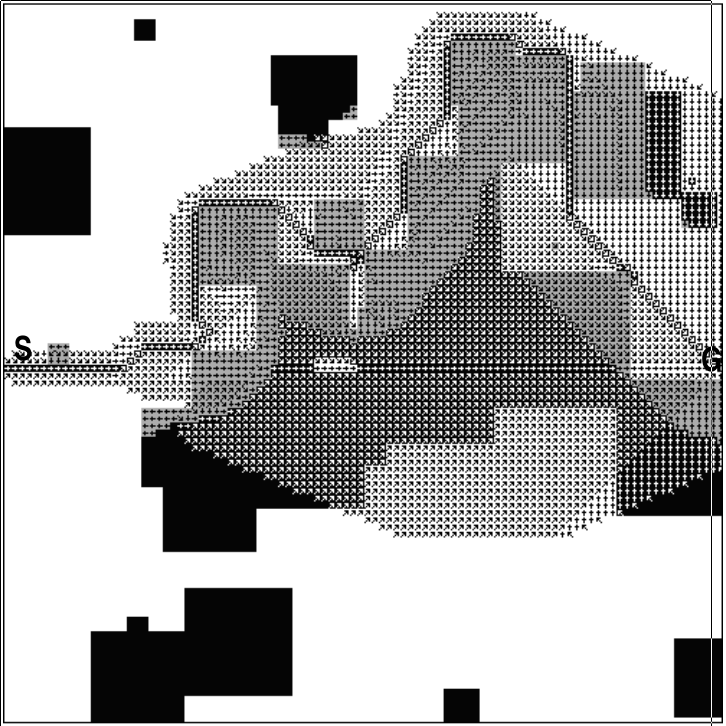
\includegraphics[width=3cm]{figs/dstar.png}};
      
      \node[anchor=north] at (7.6,7.6) {\begin{minipage}{8.5cm}
         \begin{itemize}
         \raggedright
         \item An agent conducting a traversal continually
         replans an optimal path in response to updated edge weights
         (e.g. via robot sensors).
         
         \only<2->{
         \item Algorithms: D*, Focussed D*, D* Lite.
         }
         
         \only<3->{
         \item Changed edges are treated as a property of the problem
         domain.
         }
         \end{itemize}
      \end{minipage}};
      
      \only<4->{
      \node[fill=blue!10,draw=blue!20,anchor=north,rounded corners] at (6,4.2)
      {\begin{minipage}{9.0cm}
         In contrast,
         the expensive-evaluation pathfinding problem allows for
         edges to be evaluated arbitrarily.
      \end{minipage}};
      }
      
      \only<5->{
      \node[fill=blue!10,draw=blue!20,anchor=north,rounded corners] at (6,2.9)
      {\begin{minipage}{9cm}
         LazySP exploits this freedom to focus its evaluations
         via appropriate choice of the \emph{edge selector}.
      \end{minipage}};
      }
      
      \only<2->{
      \node[inner sep=0pt] at (6,0.8) {\begin{minipage}{11.5cm}\scriptsize{
         \hangindent=0.35cm \raggedright
         \PaperPortrait\; Stentz,
         ``Optimal and Efficient Path Planning for Partially-Known
         Environments,'' ICRA 1994.
         
         \hangindent=0.35cm \raggedright
         \PaperPortrait\; Stentz,
         ``The Focussed {D}* Algorithm for Real-Time Replanning,''
         IJCAI 1995.
         
         \hangindent=0.35cm \raggedright
         \PaperPortrait\; Koenig and Likhachev,
         ``D* Lite,'' AAAI 2002.
      }\end{minipage}};
      }
      
   \end{tikzpicture}
\end{frame}

\begin{frame}
   \frametitle{Edge Selectors and Equivalences}
   \begin{tikzpicture}[font=\small]
   \draw[step=1,black!15,very thin,opacity=\gridopacity] (0,0) grid (12,8);
   \tikzset{>=latex}

   \node at (2.8,7.7) {LazySP Selector};

   \node at (7.2,7.7) {Illustration};

   \node at (10.5,7.7) {Notes};

   % Expand
   \only<2->{

   % Expand definition
   \node[fill=blue!10,draw=blue!20,rounded corners,
      minimum width=5.4cm,minimum height=0.9cm] (blockexp) at (2.8,7.0) {};
   \node[anchor=north,below=0cm of blockexp.north]
   {\begin{minipage}{5.1cm}
      \textbf{Expand}
      
      (all out-edges of frontier vertex)
   \end{minipage}};

   % Expand visualization
   \fill[blue!5,draw=blue!10,rounded corners] (5.7,6.55) rectangle (8.7,7.45);
   \begin{scope}[shift={(6.1,6.65)}]
   \begin{scope}[scale=0.25]
   
      % graph start
      \coordinate (va) at ( 0.5,0.8);
      \coordinate (vb) at ( 2.0,1.5);
      \coordinate (vc) at ( 2.5,2.7);
      \coordinate (vd) at ( 4.0,1.3);
      \coordinate (ve) at ( 6.5,1.8);
      \coordinate (vf) at ( 8.5,0.8);
      \coordinate (vg) at ( 0.0,1.8);
      \coordinate (vh) at ( 2.5,0.3);
      \coordinate (vi) at ( 5.5,0.0);
      \coordinate (vj) at ( 5.0,2.3);
      \coordinate (vk) at ( 7.5,0.3);
      
      % start/goal highlighting
      \node[circle,fill=black!20,inner sep=0.1cm] at (va) {};
      \node[circle,fill=black!20,inner sep=0.1cm] at (vf) {};
      
      \only<3->{
      % candidate path
      \draw[line width=0.2cm,color=black!30,line cap=round]
         (va) -- (vb) -- (vd) -- (ve) -- (vf);
      }
      
      \only<4->{
      % highlight first unevaled edge
      \draw[line width=0.4cm,color=blue!50!white,line cap=round] (vb) -- (vd);
      \draw[line width=0.2cm,color=black!30,line cap=round] (vb) -- (vd);
      }
      
      \only<5->{
      % point to frontier vertex
      \draw[blue!50!white,->,ultra thick] (0.5,3.0) -- (1.5,2.0);
      }
      
      % edges
      \draw[black,ultra thick] (va) -- (vb);
      \draw[black!30] (vb) -- (vd);
      \draw[black,ultra thick] (va) -- (vh);
      \draw[black!30] (vh) -- (vd);
      \draw[black!30] (vb) -- (vc);
      \draw[black!30] (vc) -- (vj);
      \draw[black,ultra thick] (va) -- (vg);
      \draw[black!30] (vb) -- (vg);
      \draw[black!30] (vb) -- (vh);
      \draw[black!30] (vc) -- (vd);
      \draw[black!30] (vd) -- (ve);
      \draw[black!30] (ve) -- (vf);
      \draw[black!30] (vd) -- (vi);
      \draw[black!30] (ve) -- (vi);
      \draw[black!30] (vd) -- (vj);
      \draw[black!30] (ve) -- (vj);
      \draw[black!30] (vf) -- (vk);
      \draw[black!30] (vi) -- (vk);
      \draw[black!30] (ve) -- (vk);
      
      \only<6->{
      % highlight edges to return
      \draw[blue,ultra thick] (va) -- (vb);
      \draw[blue,ultra thick] (vb) -- (vc);
      \draw[blue,ultra thick] (vb) -- (vd);
      \draw[blue,ultra thick] (vb) -- (vg);
      \draw[blue,ultra thick] (vb) -- (vh);
      }
      
      % nodes
      \node[circle,fill=black,inner sep=0.05cm] at (va) {};
      \node[circle,fill=black,inner sep=0.05cm] at (vb) {};
      \node[circle,fill=black,inner sep=0.05cm] at (vc) {};
      \node[circle,fill=black,inner sep=0.05cm] at (vd) {};
      \node[circle,fill=black,inner sep=0.05cm] at (ve) {};
      \node[circle,fill=black,inner sep=0.05cm] at (vf) {};
      \node[circle,fill=black,inner sep=0.05cm] at (vg) {};
      \node[circle,fill=black,inner sep=0.05cm] at (vh) {};
      \node[circle,fill=black,inner sep=0.05cm] at (vi) {};
      \node[circle,fill=black,inner sep=0.05cm] at (vj) {};
      \node[circle,fill=black,inner sep=0.05cm] at (vk) {};
   \end{scope}
   \end{scope}
   }

   \only<7->{
      % Expand notes
      \node[fill=blue!10,draw=blue!20,rounded corners,
         minimum width=3.0cm,minimum height=0.9cm,align=center] (blockexp) at (10.4,7.0)
      {Edge-equivalent to\\Weighted A* (JIT)};

      \node[anchor=west,font=\scriptsize,inner sep=0pt] at (0.25,0.6) {\begin{minipage}{10cm}
      \hangindent=0.3cm \raggedright
         \PaperPortrait\; Pohl,
         ``Heuristic Search Viewed as Path Finding in a Graph,''
         AI 1970.
      \end{minipage}};
   }

   % Forward
   \only<8->{

   % Forward definition
   \node[fill=blue!10,draw=blue!20,rounded corners,
      minimum width=5.4cm,minimum height=0.9cm] (blockexp) at (2.8,5.9) {};
   \node[anchor=north,below=0cm of blockexp.north]
   {\begin{minipage}{5.1cm}
      \textbf{Forward}
      
      (first unevaluated edge)
   \end{minipage}};

   % Forward visualization
   \fill[blue!5,draw=blue!10,rounded corners] (5.7,5.45) rectangle (8.7,6.35);
   \begin{scope}[shift={(6.1,5.55)}]
   \begin{scope}[scale=0.25]

      % graph start
      \coordinate (va) at ( 0.5,0.8);
      \coordinate (vb) at ( 2.0,1.5);
      \coordinate (vc) at ( 2.5,2.7);
      \coordinate (vd) at ( 4.0,1.3);
      \coordinate (ve) at ( 6.5,1.8);
      \coordinate (vf) at ( 8.5,0.8);
      \coordinate (vg) at ( 0.0,1.8);
      \coordinate (vh) at ( 2.5,0.3);
      \coordinate (vi) at ( 5.5,0.0);
      \coordinate (vj) at ( 5.0,2.3);
      \coordinate (vk) at ( 7.5,0.3);
      
      % start/goal highlighting
      \node[circle,fill=black!20,inner sep=0.1cm] at (va) {};
      \node[circle,fill=black!20,inner sep=0.1cm] at (vf) {};
      
      \only<9->{
      % candidate path
      \draw[line width=0.2cm,color=black!30,line cap=round]
         (va) -- (vb) -- (vd) -- (ve) -- (vf);
      }
      
      \only<10->{
      % highlight first unevaled edge
      \draw[line width=0.4cm,color=blue!50!white,line cap=round] (vb) -- (vd);
      \draw[line width=0.2cm,color=black!30,line cap=round] (vb) -- (vd);
      }
      
      % edges
      \draw[black,ultra thick] (va) -- (vb);
      \draw[black!30] (vb) -- (vd);
      \draw[black,ultra thick] (va) -- (vh);
      \draw[black!30] (vh) -- (vd);
      \draw[black!30] (vb) -- (vc);
      \draw[black!30] (vc) -- (vj);
      \draw[black,ultra thick] (va) -- (vg);
      \draw[black!30] (vb) -- (vg);
      \draw[black!30] (vb) -- (vh);
      \draw[black!30] (vc) -- (vd);
      \draw[black!30] (vd) -- (ve);
      \draw[black!30] (ve) -- (vf);
      \draw[black!30] (vd) -- (vi);
      \draw[black!30] (ve) -- (vi);
      \draw[black!30] (vd) -- (vj);
      \draw[black!30] (ve) -- (vj);
      \draw[black!30] (vf) -- (vk);
      \draw[black!30] (vi) -- (vk);
      \draw[black!30] (ve) -- (vk);
      
      \only<10->{
      % highlight edges to return
      \draw[blue,ultra thick] (vb) -- (vd);
      }
      
      % nodes
      \node[circle,fill=black,inner sep=0.05cm] at (va) {};
      \node[circle,fill=black,inner sep=0.05cm] at (vb) {};
      \node[circle,fill=black,inner sep=0.05cm] at (vc) {};
      \node[circle,fill=black,inner sep=0.05cm] at (vd) {};
      \node[circle,fill=black,inner sep=0.05cm] at (ve) {};
      \node[circle,fill=black,inner sep=0.05cm] at (vf) {};
      \node[circle,fill=black,inner sep=0.05cm] at (vg) {};
      \node[circle,fill=black,inner sep=0.05cm] at (vh) {};
      \node[circle,fill=black,inner sep=0.05cm] at (vi) {};
      \node[circle,fill=black,inner sep=0.05cm] at (vj) {};
      \node[circle,fill=black,inner sep=0.05cm] at (vk) {};
   \end{scope}
   \end{scope}
   }

   \only<11->{
      % Forward notes
      \node[fill=blue!10,draw=blue!20,rounded corners,
         minimum width=3.0cm,minimum height=0.9cm,align=center] (blockexp) at (10.4,5.9)
      {Edge-equivalent to\\Lazy Weighted A*};

      \node[anchor=west,font=\scriptsize,inner sep=0pt] at (0.25,0.2) {\begin{minipage}{11.5cm}
      \hangindent=0.3cm \raggedright
         \PaperPortrait\; Cohen, Phillips, and Likhachev,
         ``Planning Single-arm Manipulations with n-Arm Robots,''
         RSS 2014.
      \end{minipage}};
   }


   % Reverse
   \only<12->{

   % Reverse definition
   \node[fill=blue!10,draw=blue!20,rounded corners,
      minimum width=5.4cm,minimum height=0.9cm] (blockexp) at (2.8,4.8) {};
   \node[anchor=north,below=0cm of blockexp.north]
   {\begin{minipage}{5.1cm}
      \textbf{Reverse}
      
      (last unevaluated edge)
   \end{minipage}};

   % Reverse visualization
   \fill[blue!5,draw=blue!10,rounded corners] (5.7,4.35) rectangle (8.7,5.25);
   \begin{scope}[shift={(6.1,4.45)}]
   \begin{scope}[scale=0.25]
   
      % graph start
      \coordinate (va) at ( 0.5,0.8);
      \coordinate (vb) at ( 2.0,1.5);
      \coordinate (vc) at ( 2.5,2.7);
      \coordinate (vd) at ( 4.0,1.3);
      \coordinate (ve) at ( 6.5,1.8);
      \coordinate (vf) at ( 8.5,0.8);
      \coordinate (vg) at ( 0.0,1.8);
      \coordinate (vh) at ( 2.5,0.3);
      \coordinate (vi) at ( 5.5,0.0);
      \coordinate (vj) at ( 5.0,2.3);
      \coordinate (vk) at ( 7.5,0.3);
      
      % start/goal highlighting
      \node[circle,fill=black!20,inner sep=0.1cm] at (va) {};
      \node[circle,fill=black!20,inner sep=0.1cm] at (vf) {};
      
      % candidate path
      \draw[line width=0.2cm,color=black!30,line cap=round]
         (va) -- (vb) -- (vd) -- (ve) -- (vf);
      
      % highlight first unevaled edge
      \draw[line width=0.4cm,color=blue!50!white,line cap=round] (ve) -- (vf);
      \draw[line width=0.2cm,color=black!30,line cap=round] (ve) -- (vf);
      
      % edges
      \draw[black,ultra thick] (va) -- (vb);
      \draw[black!30] (vb) -- (vd);
      \draw[black,ultra thick] (va) -- (vh);
      \draw[black!30] (vh) -- (vd);
      \draw[black!30] (vb) -- (vc);
      \draw[black!30] (vc) -- (vj);
      \draw[black,ultra thick] (va) -- (vg);
      \draw[black!30] (vb) -- (vg);
      \draw[black!30] (vb) -- (vh);
      \draw[black!30] (vc) -- (vd);
      \draw[black!30] (vd) -- (ve);
      \draw[black!30] (ve) -- (vf);
      \draw[black!30] (vd) -- (vi);
      \draw[black!30] (ve) -- (vi);
      \draw[black!30] (vd) -- (vj);
      \draw[black!30] (ve) -- (vj);
      \draw[black!30] (vf) -- (vk);
      \draw[black!30] (vi) -- (vk);
      \draw[black!30] (ve) -- (vk);
      
      \draw[blue,ultra thick] (ve) -- (vf);
      
      % nodes
      \node[circle,fill=black,inner sep=0.05cm] at (va) {};
      \node[circle,fill=black,inner sep=0.05cm] at (vb) {};
      \node[circle,fill=black,inner sep=0.05cm] at (vc) {};
      \node[circle,fill=black,inner sep=0.05cm] at (vd) {};
      \node[circle,fill=black,inner sep=0.05cm] at (ve) {};
      \node[circle,fill=black,inner sep=0.05cm] at (vf) {};
      \node[circle,fill=black,inner sep=0.05cm] at (vg) {};
      \node[circle,fill=black,inner sep=0.05cm] at (vh) {};
      \node[circle,fill=black,inner sep=0.05cm] at (vi) {};
      \node[circle,fill=black,inner sep=0.05cm] at (vj) {};
      \node[circle,fill=black,inner sep=0.05cm] at (vk) {};
   \end{scope}
   \end{scope}
   }


   % Alternate
   \only<13->{

   % Alternate definition
   \node[fill=blue!10,draw=blue!20,rounded corners,
      minimum width=5.4cm,minimum height=0.9cm] (blockexp) at (2.8,3.7) {};
   \node[anchor=north,below=0cm of blockexp.north]
   {\begin{minipage}{5.1cm}
      \textbf{Alternate}
      
      (alternate Forward and Reverse)
   \end{minipage}};

   % Alternate visualization
   \fill[blue!5,draw=blue!10,rounded corners] (5.7,3.25) rectangle (8.7,4.15);
   \begin{scope}[shift={(6.1,3.35)}]
   \begin{scope}[scale=0.25]

      % graph start
      \coordinate (va) at ( 0.5,0.8);
      \coordinate (vb) at ( 2.0,1.5);
      \coordinate (vc) at ( 2.5,2.7);
      \coordinate (vd) at ( 4.0,1.3);
      \coordinate (ve) at ( 6.5,1.8);
      \coordinate (vf) at ( 8.5,0.8);
      \coordinate (vg) at ( 0.0,1.8);
      \coordinate (vh) at ( 2.5,0.3);
      \coordinate (vi) at ( 5.5,0.0);
      \coordinate (vj) at ( 5.0,2.3);
      \coordinate (vk) at ( 7.5,0.3);
      
      % start/goal highlighting
      \node[circle,fill=black!20,inner sep=0.1cm] at (va) {};
      \node[circle,fill=black!20,inner sep=0.1cm] at (vf) {};
      
      % candidate path
      \draw[line width=0.2cm,color=black!30,line cap=round]
         (va) -- (vb) -- (vd) -- (ve) -- (vf);
      
      \only<14>{
      % highlight first unevaled edge
      \draw[line width=0.4cm,color=blue!50!white,line cap=round] (vb) -- (vd);
      \draw[line width=0.2cm,color=black!30,line cap=round] (vb) -- (vd);
      }
      \only<15>{
      % highlight first unevaled edge
      \draw[line width=0.4cm,color=blue!50!white,line cap=round] (ve) -- (vf);
      \draw[line width=0.2cm,color=black!30,line cap=round] (ve) -- (vf);
      }
      \only<16->{
      % highlight first unevaled edge
      \draw[line width=0.4cm,color=blue!50!white,line cap=round] (vd) -- (ve);
      \draw[line width=0.2cm,color=black!30,line cap=round] (vd) -- (ve);
      }
      
      % edges
      \draw[black,ultra thick] (va) -- (vb);
      \draw[black!30] (vb) -- (vd);
      \draw[black,ultra thick] (va) -- (vh);
      \draw[black!30] (vh) -- (vd);
      \draw[black!30] (vb) -- (vc);
      \draw[black!30] (vc) -- (vj);
      \draw[black,ultra thick] (va) -- (vg);
      \draw[black!30] (vb) -- (vg);
      \draw[black!30] (vb) -- (vh);
      \draw[black!30] (vc) -- (vd);
      \draw[black!30] (vd) -- (ve);
      \draw[black!30] (ve) -- (vf);
      \draw[black!30] (vd) -- (vi);
      \draw[black!30] (ve) -- (vi);
      \draw[black!30] (vd) -- (vj);
      \draw[black!30] (ve) -- (vj);
      \draw[black!30] (vf) -- (vk);
      \draw[black!30] (vi) -- (vk);
      \draw[black!30] (ve) -- (vk);
      
      % highlight edges to return
      \only<14>{\draw[blue,ultra thick] (vb) -- (vd);}
      \only<15->{\draw[black,ultra thick] (vb) -- (vd);}
      \only<15>{\draw[blue,ultra thick] (ve) -- (vf);}
      \only<16->{\draw[black,ultra thick] (ve) -- (vf);}
      \only<16->{\draw[blue,ultra thick] (vd) -- (ve);}
      
      % nodes
      \node[circle,fill=black,inner sep=0.05cm] at (va) {};
      \node[circle,fill=black,inner sep=0.05cm] at (vb) {};
      \node[circle,fill=black,inner sep=0.05cm] at (vc) {};
      \node[circle,fill=black,inner sep=0.05cm] at (vd) {};
      \node[circle,fill=black,inner sep=0.05cm] at (ve) {};
      \node[circle,fill=black,inner sep=0.05cm] at (vf) {};
      \node[circle,fill=black,inner sep=0.05cm] at (vg) {};
      \node[circle,fill=black,inner sep=0.05cm] at (vh) {};
      \node[circle,fill=black,inner sep=0.05cm] at (vi) {};
      \node[circle,fill=black,inner sep=0.05cm] at (vj) {};
      \node[circle,fill=black,inner sep=0.05cm] at (vk) {};
   \end{scope}
   \end{scope}
   }


   % Bisect
   \only<17->{

   % Bisect definition
   \node[fill=blue!10,draw=blue!20,rounded corners,
      minimum width=5.4cm,minimum height=0.9cm] (blockexp) at (2.8,2.6) {};
   \node[anchor=north,below=0cm of blockexp.north]
   {\begin{minipage}{5.1cm}
      \textbf{Bisect}
      
      (furthest from an unevaluated edge)
   \end{minipage}};

   % Bisect visualization
   \fill[blue!5,draw=blue!10,rounded corners] (5.7,2.15) rectangle (8.7,3.05);
   \begin{scope}[shift={(6.1,2.25)}]
   \begin{scope}[scale=0.25]

      % graph start
      \coordinate (va) at ( 0.5,0.8);
      \coordinate (vb) at ( 2.0,1.5);
      \coordinate (vc) at ( 2.5,2.7);
      \coordinate (vd) at ( 4.0,1.3);
      \coordinate (ve) at ( 6.5,1.8);
      \coordinate (vf) at ( 8.5,0.8);
      \coordinate (vg) at ( 0.0,1.8);
      \coordinate (vh) at ( 2.5,0.3);
      \coordinate (vi) at ( 5.5,0.0);
      \coordinate (vj) at ( 5.0,2.3);
      \coordinate (vk) at ( 7.5,0.3);
      
      % start/goal highlighting
      \node[circle,fill=black!20,inner sep=0.1cm] at (va) {};
      \node[circle,fill=black!20,inner sep=0.1cm] at (vf) {};
      
      % candidate path
      \draw[line width=0.2cm,color=black!30,line cap=round]
         (va) -- (vb) -- (vd) -- (ve) -- (vf);
      
      % highlight first unevaled edge
      \draw[line width=0.4cm,color=blue!50!white,line cap=round] (vd) -- (ve);
      \draw[line width=0.2cm,color=black!30,line cap=round] (vd) -- (ve);
      
      % edges
      \draw[black,ultra thick] (va) -- (vb);
      \draw[black!30] (vb) -- (vd);
      \draw[black,ultra thick] (va) -- (vh);
      \draw[black!30] (vh) -- (vd);
      \draw[black!30] (vb) -- (vc);
      \draw[black!30] (vc) -- (vj);
      \draw[black,ultra thick] (va) -- (vg);
      \draw[black!30] (vb) -- (vg);
      \draw[black!30] (vb) -- (vh);
      \draw[black!30] (vc) -- (vd);
      \draw[black!30] (vd) -- (ve);
      \draw[black!30] (ve) -- (vf);
      \draw[black!30] (vd) -- (vi);
      \draw[black!30] (ve) -- (vi);
      \draw[black!30] (vd) -- (vj);
      \draw[black!30] (ve) -- (vj);
      \draw[black!30] (vf) -- (vk);
      \draw[black!30] (vi) -- (vk);
      \draw[black!30] (ve) -- (vk);
      
      % highlight edges to return
      \draw[black,ultra thick] (vd) -- (ve);
      
      % nodes
      \node[circle,fill=black,inner sep=0.05cm] at (va) {};
      \node[circle,fill=black,inner sep=0.05cm] at (vb) {};
      \node[circle,fill=black,inner sep=0.05cm] at (vc) {};
      \node[circle,fill=black,inner sep=0.05cm] at (vd) {};
      \node[circle,fill=black,inner sep=0.05cm] at (ve) {};
      \node[circle,fill=black,inner sep=0.05cm] at (vf) {};
      \node[circle,fill=black,inner sep=0.05cm] at (vg) {};
      \node[circle,fill=black,inner sep=0.05cm] at (vh) {};
      \node[circle,fill=black,inner sep=0.05cm] at (vi) {};
      \node[circle,fill=black,inner sep=0.05cm] at (vj) {};
      \node[circle,fill=black,inner sep=0.05cm] at (vk) {};
   \end{scope}
   \end{scope}
   }


   % Most Likely
   \only<18->{

   % Most definition
   \node[fill=blue!10,draw=blue!20,rounded corners,
      minimum width=11.8cm,minimum height=0.9cm] (blockexp) at (6.0,1.5) {};
   \node[anchor=north,below=0cm of blockexp.north]
   {\begin{minipage}{11.5cm}
      Novel selectors: \textbf{Path Distribution}
      
      (most likely on a shortest path drawn from $\mathcal{D}_p$)
   \end{minipage}};
   }
   
   \end{tikzpicture}
\end{frame}








%\begin{frame}
   %\frametitle{Simple Edge Selectors and Equivalences}
   %\begin{tikzpicture}
      %\draw[step=1,black!15,very thin,opacity=\gridopacity] (0,0) grid (12,8);
      %\tikzset{>=latex}
   
   
      %\only<2->{
      %\node[fill=blue!20,anchor=north,rounded corners,
         %minimum width=5.8cm,minimum height=3cm] (blockexp) at (3,7.8) {};
      %\node[anchor=north,below=0cm of blockexp.north]
      %{\begin{minipage}{5.5cm}
         %\textbf{LazySP w/ Expand Selector}
         
         %(all out-edges of frontier vertex)
      %\end{minipage}};
      %\begin{scope}[scale=0.5,shift={(1.75,10.2)}]
      
         %\fill[white,opacity=0.7,rounded corners] (-1.3,-0.4) rectangle (9.8,3.2);
      
         %% graph start
         %\coordinate (va) at ( 0.5,0.8);
         %\coordinate (vb) at ( 2.0,1.5);
         %\coordinate (vc) at ( 2.5,2.7);
         %\coordinate (vd) at ( 4.0,1.3);
         %\coordinate (ve) at ( 6.5,1.8);
         %\coordinate (vf) at ( 8.5,0.8);
         %\coordinate (vg) at ( 0.0,1.8);
         %\coordinate (vh) at ( 2.5,0.3);
         %\coordinate (vi) at ( 5.5,0.0);
         %\coordinate (vj) at ( 5.0,2.3);
         %\coordinate (vk) at ( 7.5,0.3);
         
         %% start/goal highlighting
         %\node[circle,fill=black!20,inner sep=0.1cm] at (va) {};
         %\node[circle,fill=black!20,inner sep=0.1cm] at (vf) {};
         
         %\only<3->{
         %% candidate path
         %\draw[line width=0.2cm,color=black!30,line cap=round]
            %(va) -- (vb) -- (vd) -- (ve) -- (vf);
         %}
         
         %\only<4->{
         %% highlight first unevaled edge
         %\draw[line width=0.4cm,color=blue!50!white,line cap=round] (vb) -- (vd);
         %\draw[line width=0.2cm,color=black!30,line cap=round] (vb) -- (vd);
         %}
         
         %\only<5->{
         %% point to frontier vertex
         %\draw[blue!50!white,->,ultra thick] (0.5,3.0) -- (1.5,2.0);
         %}
         
         %% edges
         %\draw[black,ultra thick] (va) -- (vb);
         %\draw[black!30] (vb) -- (vd);
         %\draw[black,ultra thick] (va) -- (vh);
         %\draw[black!30] (vh) -- (vd);
         %\draw[black!30] (vb) -- (vc);
         %\draw[black!30] (vc) -- (vj);
         %\draw[black,ultra thick] (va) -- (vg);
         %\draw[black!30] (vb) -- (vg);
         %\draw[black!30] (vb) -- (vh);
         %\draw[black!30] (vc) -- (vd);
         %\draw[black!30] (vd) -- (ve);
         %\draw[black!30] (ve) -- (vf);
         %\draw[black!30] (vd) -- (vi);
         %\draw[black!30] (ve) -- (vi);
         %\draw[black!30] (vd) -- (vj);
         %\draw[black!30] (ve) -- (vj);
         %\draw[black!30] (vf) -- (vk);
         %\draw[black!30] (vi) -- (vk);
         %\draw[black!30] (ve) -- (vk);
         
         %\only<6->{
         %% highlight edges to return
         %\draw[blue,ultra thick] (va) -- (vb);
         %\draw[blue,ultra thick] (vb) -- (vc);
         %\draw[blue,ultra thick] (vb) -- (vd);
         %\draw[blue,ultra thick] (vb) -- (vg);
         %\draw[blue,ultra thick] (vb) -- (vh);
         %}
         
         %% nodes
         %\node[circle,fill=black,inner sep=0.05cm] at (va) {};
         %\node[circle,fill=black,inner sep=0.05cm] at (vb) {};
         %\node[circle,fill=black,inner sep=0.05cm] at (vc) {};
         %\node[circle,fill=black,inner sep=0.05cm] at (vd) {};
         %\node[circle,fill=black,inner sep=0.05cm] at (ve) {};
         %\node[circle,fill=black,inner sep=0.05cm] at (vf) {};
         %\node[circle,fill=black,inner sep=0.05cm] at (vg) {};
         %\node[circle,fill=black,inner sep=0.05cm] at (vh) {};
         %\node[circle,fill=black,inner sep=0.05cm] at (vi) {};
         %\node[circle,fill=black,inner sep=0.05cm] at (vj) {};
         %\node[circle,fill=black,inner sep=0.05cm] at (vk) {};
      %\end{scope}
      %}
      %\only<7->{
      %\node[fill=blue!20,anchor=north,rounded corners,
         %minimum width=5.8cm,minimum height=3cm] (blockexp) at (9,7.8) {};
      %\node[anchor=north,below=0cm of blockexp.north]
      %{\begin{minipage}{5.5cm}
         %\textbf{Weighted A*}
         
         %with JIT/memoized evaluations
         
      %\end{minipage}};
      %\node[anchor=south,above=0cm of blockexp.south]
      %{\begin{minipage}{5.5cm}\scriptsize
      
         %\hangindent=0.35cm \raggedright
         %\PaperPortrait\; Pohl,
         %``Heuristic Search Viewed as Path Finding in a Graph,''
         %AI 1970.
      
      %\end{minipage}};
      %\node[fill=white,opacity=0.9,inner sep=0.1cm,rounded corners] at (6,6.3) {\LARGE =};
      %}
      
      
      
      %\only<8->{
      %\node[fill=blue!20,anchor=north,rounded corners,
         %minimum width=5.8cm,minimum height=3cm] (blockfwd) at (3,4.5) {};
      %\node[anchor=north,below=0cm of blockfwd.north]
      %{\begin{minipage}{5.5cm}
         %\textbf{LazySP w/ Forward Selector}
         
         %(first unevaluated edge)
      %\end{minipage}};
      %\begin{scope}[scale=0.5,shift={(1.75,3.6)}]
      
         %\fill[white,opacity=0.7,rounded corners] (-1.3,-0.4) rectangle (9.8,3.2);
      
         %% graph start
         %\coordinate (va) at ( 0.5,0.8);
         %\coordinate (vb) at ( 2.0,1.5);
         %\coordinate (vc) at ( 2.5,2.7);
         %\coordinate (vd) at ( 4.0,1.3);
         %\coordinate (ve) at ( 6.5,1.8);
         %\coordinate (vf) at ( 8.5,0.8);
         %\coordinate (vg) at ( 0.0,1.8);
         %\coordinate (vh) at ( 2.5,0.3);
         %\coordinate (vi) at ( 5.5,0.0);
         %\coordinate (vj) at ( 5.0,2.3);
         %\coordinate (vk) at ( 7.5,0.3);
         
         %% start/goal highlighting
         %\node[circle,fill=black!20,inner sep=0.1cm] at (va) {};
         %\node[circle,fill=black!20,inner sep=0.1cm] at (vf) {};
         
         %\only<9->{
         %% candidate path
         %\draw[line width=0.2cm,color=black!30,line cap=round]
            %(va) -- (vb) -- (vd) -- (ve) -- (vf);
         %}
         
         %\only<10->{
         %% highlight first unevaled edge
         %\draw[line width=0.4cm,color=blue!50!white,line cap=round] (vb) -- (vd);
         %\draw[line width=0.2cm,color=black!30,line cap=round] (vb) -- (vd);
         %}
         
         %% edges
         %\draw[black,ultra thick] (va) -- (vb);
         %\draw[black!30] (vb) -- (vd);
         %\draw[black,ultra thick] (va) -- (vh);
         %\draw[black!30] (vh) -- (vd);
         %\draw[black!30] (vb) -- (vc);
         %\draw[black!30] (vc) -- (vj);
         %\draw[black,ultra thick] (va) -- (vg);
         %\draw[black!30] (vb) -- (vg);
         %\draw[black!30] (vb) -- (vh);
         %\draw[black!30] (vc) -- (vd);
         %\draw[black!30] (vd) -- (ve);
         %\draw[black!30] (ve) -- (vf);
         %\draw[black!30] (vd) -- (vi);
         %\draw[black!30] (ve) -- (vi);
         %\draw[black!30] (vd) -- (vj);
         %\draw[black!30] (ve) -- (vj);
         %\draw[black!30] (vf) -- (vk);
         %\draw[black!30] (vi) -- (vk);
         %\draw[black!30] (ve) -- (vk);
         
         %\only<10->{
         %% highlight edges to return
         %\draw[blue,ultra thick] (vb) -- (vd);
         %}
         
         %% nodes
         %\node[circle,fill=black,inner sep=0.05cm] at (va) {};
         %\node[circle,fill=black,inner sep=0.05cm] at (vb) {};
         %\node[circle,fill=black,inner sep=0.05cm] at (vc) {};
         %\node[circle,fill=black,inner sep=0.05cm] at (vd) {};
         %\node[circle,fill=black,inner sep=0.05cm] at (ve) {};
         %\node[circle,fill=black,inner sep=0.05cm] at (vf) {};
         %\node[circle,fill=black,inner sep=0.05cm] at (vg) {};
         %\node[circle,fill=black,inner sep=0.05cm] at (vh) {};
         %\node[circle,fill=black,inner sep=0.05cm] at (vi) {};
         %\node[circle,fill=black,inner sep=0.05cm] at (vj) {};
         %\node[circle,fill=black,inner sep=0.05cm] at (vk) {};
      %\end{scope}
      %}
      
      %\only<11->{
      %\node[fill=blue!20,anchor=north,rounded corners,
         %minimum width=5.8cm,minimum height=3cm] (blockexp) at (9,4.5) {};
      %\node[anchor=north,below=0cm of blockexp.north]
      %{\begin{minipage}{5.5cm}
         %\textbf{Lazy Weighted A*}
         
         %with JIT/memoized evaluations
         
      %\end{minipage}};
      %\node[anchor=south,above=0cm of blockexp.south]
      %{\begin{minipage}{5.5cm}\scriptsize
      
         %\hangindent=0.35cm 
         %\PaperPortrait\; Cohen, Phillips, and Likhachev,
         %``Planning Single-arm Manipulations with n-Arm Robots,''
         %RSS 2014.
      
      %\end{minipage}};
      %\node[fill=white,opacity=0.9,inner sep=0.1cm,rounded corners] at (6,3.0) {\LARGE =};
      %}
      
      %\only<7->{
      %\node[fill=black!20,rounded corners] at (6,0.75)
      %{\begin{minipage}{7.3cm}
         %Edge-equivalence: algorithms will evaluate
         %the same edges in the same order.
      %\end{minipage}};
      %}
   
   %\end{tikzpicture}
%\end{frame}

%\begin{frame}
   %\frametitle{Other Simple Edge Selectors}
   %\begin{tikzpicture}
      %\draw[step=1,black!15,very thin,opacity=\gridopacity] (0,0) grid (12,8);
      %\tikzset{>=latex}
      
      
      
      %\node[fill=blue!20,anchor=north,rounded corners,
         %minimum width=5.8cm,minimum height=3cm] (blockexp) at (3,7.8) {};
      %\node[anchor=north,below=0cm of blockexp.north]
      %{\begin{minipage}{5.5cm}
         %\textbf{LazySP w/ Forward Selector}
         
         %(first unevaluated edge)
      %\end{minipage}};
      %\begin{scope}[scale=0.5,shift={(1.75,10.2)}]
      
         %\fill[white,opacity=0.7,rounded corners] (-1.3,-0.4) rectangle (9.8,3.2);
      
         %% graph start
         %\coordinate (va) at ( 0.5,0.8);
         %\coordinate (vb) at ( 2.0,1.5);
         %\coordinate (vc) at ( 2.5,2.7);
         %\coordinate (vd) at ( 4.0,1.3);
         %\coordinate (ve) at ( 6.5,1.8);
         %\coordinate (vf) at ( 8.5,0.8);
         %\coordinate (vg) at ( 0.0,1.8);
         %\coordinate (vh) at ( 2.5,0.3);
         %\coordinate (vi) at ( 5.5,0.0);
         %\coordinate (vj) at ( 5.0,2.3);
         %\coordinate (vk) at ( 7.5,0.3);
         
         %% start/goal highlighting
         %\node[circle,fill=black!20,inner sep=0.1cm] at (va) {};
         %\node[circle,fill=black!20,inner sep=0.1cm] at (vf) {};
         
         %% candidate path
         %\draw[line width=0.2cm,color=black!30,line cap=round]
            %(va) -- (vb) -- (vd) -- (ve) -- (vf);
         
         %% highlight first unevaled edge
         %\draw[line width=0.4cm,color=blue!50!white,line cap=round] (vb) -- (vd);
         %\draw[line width=0.2cm,color=black!30,line cap=round] (vb) -- (vd);
         
         %% edges
         %\draw[black,ultra thick] (va) -- (vb);
         %\draw[black!30] (vb) -- (vd);
         %\draw[black,ultra thick] (va) -- (vh);
         %\draw[black!30] (vh) -- (vd);
         %\draw[black!30] (vb) -- (vc);
         %\draw[black!30] (vc) -- (vj);
         %\draw[black,ultra thick] (va) -- (vg);
         %\draw[black!30] (vb) -- (vg);
         %\draw[black!30] (vb) -- (vh);
         %\draw[black!30] (vc) -- (vd);
         %\draw[black!30] (vd) -- (ve);
         %\draw[black!30] (ve) -- (vf);
         %\draw[black!30] (vd) -- (vi);
         %\draw[black!30] (ve) -- (vi);
         %\draw[black!30] (vd) -- (vj);
         %\draw[black!30] (ve) -- (vj);
         %\draw[black!30] (vf) -- (vk);
         %\draw[black!30] (vi) -- (vk);
         %\draw[black!30] (ve) -- (vk);
         
         %\draw[blue,ultra thick] (vb) -- (vd);
         
         %% nodes
         %\node[circle,fill=black,inner sep=0.05cm] at (va) {};
         %\node[circle,fill=black,inner sep=0.05cm] at (vb) {};
         %\node[circle,fill=black,inner sep=0.05cm] at (vc) {};
         %\node[circle,fill=black,inner sep=0.05cm] at (vd) {};
         %\node[circle,fill=black,inner sep=0.05cm] at (ve) {};
         %\node[circle,fill=black,inner sep=0.05cm] at (vf) {};
         %\node[circle,fill=black,inner sep=0.05cm] at (vg) {};
         %\node[circle,fill=black,inner sep=0.05cm] at (vh) {};
         %\node[circle,fill=black,inner sep=0.05cm] at (vi) {};
         %\node[circle,fill=black,inner sep=0.05cm] at (vj) {};
         %\node[circle,fill=black,inner sep=0.05cm] at (vk) {};
      %\end{scope}
      
      
      
      %\only<2->{
      %\node[fill=blue!20,anchor=north,rounded corners,
         %minimum width=5.8cm,minimum height=3cm] (blockexp) at (9,7.8) {};
      %\node[anchor=north,below=0cm of blockexp.north]
      %{\begin{minipage}{5.5cm}
         %\textbf{LazySP w/ Reverse Selector}
         
         %(last unevaluated edge)
      %\end{minipage}};
      %\begin{scope}[scale=0.5,shift={(13.75,10.2)}]
      
         %\fill[white,opacity=0.7,rounded corners] (-1.3,-0.4) rectangle (9.8,3.2);
      
         %% graph start
         %\coordinate (va) at ( 0.5,0.8);
         %\coordinate (vb) at ( 2.0,1.5);
         %\coordinate (vc) at ( 2.5,2.7);
         %\coordinate (vd) at ( 4.0,1.3);
         %\coordinate (ve) at ( 6.5,1.8);
         %\coordinate (vf) at ( 8.5,0.8);
         %\coordinate (vg) at ( 0.0,1.8);
         %\coordinate (vh) at ( 2.5,0.3);
         %\coordinate (vi) at ( 5.5,0.0);
         %\coordinate (vj) at ( 5.0,2.3);
         %\coordinate (vk) at ( 7.5,0.3);
         
         %% start/goal highlighting
         %\node[circle,fill=black!20,inner sep=0.1cm] at (va) {};
         %\node[circle,fill=black!20,inner sep=0.1cm] at (vf) {};
         
         %% candidate path
         %\draw[line width=0.2cm,color=black!30,line cap=round]
            %(va) -- (vb) -- (vd) -- (ve) -- (vf);
         
         %% highlight first unevaled edge
         %\draw[line width=0.4cm,color=blue!50!white,line cap=round] (ve) -- (vf);
         %\draw[line width=0.2cm,color=black!30,line cap=round] (ve) -- (vf);
         
         %% edges
         %\draw[black,ultra thick] (va) -- (vb);
         %\draw[black!30] (vb) -- (vd);
         %\draw[black,ultra thick] (va) -- (vh);
         %\draw[black!30] (vh) -- (vd);
         %\draw[black!30] (vb) -- (vc);
         %\draw[black!30] (vc) -- (vj);
         %\draw[black,ultra thick] (va) -- (vg);
         %\draw[black!30] (vb) -- (vg);
         %\draw[black!30] (vb) -- (vh);
         %\draw[black!30] (vc) -- (vd);
         %\draw[black!30] (vd) -- (ve);
         %\draw[black!30] (ve) -- (vf);
         %\draw[black!30] (vd) -- (vi);
         %\draw[black!30] (ve) -- (vi);
         %\draw[black!30] (vd) -- (vj);
         %\draw[black!30] (ve) -- (vj);
         %\draw[black!30] (vf) -- (vk);
         %\draw[black!30] (vi) -- (vk);
         %\draw[black!30] (ve) -- (vk);
         
         %\draw[blue,ultra thick] (ve) -- (vf);
         
         %% nodes
         %\node[circle,fill=black,inner sep=0.05cm] at (va) {};
         %\node[circle,fill=black,inner sep=0.05cm] at (vb) {};
         %\node[circle,fill=black,inner sep=0.05cm] at (vc) {};
         %\node[circle,fill=black,inner sep=0.05cm] at (vd) {};
         %\node[circle,fill=black,inner sep=0.05cm] at (ve) {};
         %\node[circle,fill=black,inner sep=0.05cm] at (vf) {};
         %\node[circle,fill=black,inner sep=0.05cm] at (vg) {};
         %\node[circle,fill=black,inner sep=0.05cm] at (vh) {};
         %\node[circle,fill=black,inner sep=0.05cm] at (vi) {};
         %\node[circle,fill=black,inner sep=0.05cm] at (vj) {};
         %\node[circle,fill=black,inner sep=0.05cm] at (vk) {};
      %\end{scope}
      %}
      
      
      
      %\only<3->{
      %\node[fill=blue!20,anchor=north,rounded corners,
         %minimum width=5.8cm,minimum height=3cm] (blockfwd) at (3,4.5) {};
      %\node[anchor=north,below=0cm of blockfwd.north]
      %{\begin{minipage}{5.5cm}
         %\textbf{LazySP w/ Alternate Selector}
         
         %(alternate Forward and Reverse)
      %\end{minipage}};
      %\begin{scope}[scale=0.5,shift={(1.75,3.6)}]
      
         %\fill[white,opacity=0.7,rounded corners] (-1.3,-0.4) rectangle (9.8,3.2);
      
         %% graph start
         %\coordinate (va) at ( 0.5,0.8);
         %\coordinate (vb) at ( 2.0,1.5);
         %\coordinate (vc) at ( 2.5,2.7);
         %\coordinate (vd) at ( 4.0,1.3);
         %\coordinate (ve) at ( 6.5,1.8);
         %\coordinate (vf) at ( 8.5,0.8);
         %\coordinate (vg) at ( 0.0,1.8);
         %\coordinate (vh) at ( 2.5,0.3);
         %\coordinate (vi) at ( 5.5,0.0);
         %\coordinate (vj) at ( 5.0,2.3);
         %\coordinate (vk) at ( 7.5,0.3);
         
         %% start/goal highlighting
         %\node[circle,fill=black!20,inner sep=0.1cm] at (va) {};
         %\node[circle,fill=black!20,inner sep=0.1cm] at (vf) {};
         
         %% candidate path
         %\draw[line width=0.2cm,color=black!30,line cap=round]
            %(va) -- (vb) -- (vd) -- (ve) -- (vf);
         
         %\only<4>{
         %% highlight first unevaled edge
         %\draw[line width=0.4cm,color=blue!50!white,line cap=round] (vb) -- (vd);
         %\draw[line width=0.2cm,color=black!30,line cap=round] (vb) -- (vd);
         %}
         %\only<5>{
         %% highlight first unevaled edge
         %\draw[line width=0.4cm,color=blue!50!white,line cap=round] (ve) -- (vf);
         %\draw[line width=0.2cm,color=black!30,line cap=round] (ve) -- (vf);
         %}
         %\only<6->{
         %% highlight first unevaled edge
         %\draw[line width=0.4cm,color=blue!50!white,line cap=round] (vd) -- (ve);
         %\draw[line width=0.2cm,color=black!30,line cap=round] (vd) -- (ve);
         %}
         
         %% edges
         %\draw[black,ultra thick] (va) -- (vb);
         %\draw[black!30] (vb) -- (vd);
         %\draw[black,ultra thick] (va) -- (vh);
         %\draw[black!30] (vh) -- (vd);
         %\draw[black!30] (vb) -- (vc);
         %\draw[black!30] (vc) -- (vj);
         %\draw[black,ultra thick] (va) -- (vg);
         %\draw[black!30] (vb) -- (vg);
         %\draw[black!30] (vb) -- (vh);
         %\draw[black!30] (vc) -- (vd);
         %\draw[black!30] (vd) -- (ve);
         %\draw[black!30] (ve) -- (vf);
         %\draw[black!30] (vd) -- (vi);
         %\draw[black!30] (ve) -- (vi);
         %\draw[black!30] (vd) -- (vj);
         %\draw[black!30] (ve) -- (vj);
         %\draw[black!30] (vf) -- (vk);
         %\draw[black!30] (vi) -- (vk);
         %\draw[black!30] (ve) -- (vk);
         
         %% highlight edges to return
         %\only<4>{\draw[blue,ultra thick] (vb) -- (vd);}
         %\only<5->{\draw[black,ultra thick] (vb) -- (vd);}
         %\only<5>{\draw[blue,ultra thick] (ve) -- (vf);}
         %\only<6->{\draw[black,ultra thick] (ve) -- (vf);}
         %\only<6->{\draw[blue,ultra thick] (vd) -- (ve);}
         
         %% nodes
         %\node[circle,fill=black,inner sep=0.05cm] at (va) {};
         %\node[circle,fill=black,inner sep=0.05cm] at (vb) {};
         %\node[circle,fill=black,inner sep=0.05cm] at (vc) {};
         %\node[circle,fill=black,inner sep=0.05cm] at (vd) {};
         %\node[circle,fill=black,inner sep=0.05cm] at (ve) {};
         %\node[circle,fill=black,inner sep=0.05cm] at (vf) {};
         %\node[circle,fill=black,inner sep=0.05cm] at (vg) {};
         %\node[circle,fill=black,inner sep=0.05cm] at (vh) {};
         %\node[circle,fill=black,inner sep=0.05cm] at (vi) {};
         %\node[circle,fill=black,inner sep=0.05cm] at (vj) {};
         %\node[circle,fill=black,inner sep=0.05cm] at (vk) {};
      %\end{scope}
      %}
      
      
      
      %\only<7->{
      %\node[fill=blue!20,anchor=north,rounded corners,
         %minimum width=5.8cm,minimum height=3cm] (blockfwd) at (9,4.5) {};
      %\node[anchor=north,below=0cm of blockfwd.north]
      %{\begin{minipage}{5.5cm}
         %\textbf{LazySP w/ Bisect Selector}
         
         %(alternate Forward and Reverse)
      %\end{minipage}};
      %\begin{scope}[scale=0.5,shift={(13.75,3.6)}]
      
         %\fill[white,opacity=0.7,rounded corners] (-1.3,-0.4) rectangle (9.8,3.2);
      
         %% graph start
         %\coordinate (va) at ( 0.5,0.8);
         %\coordinate (vb) at ( 2.0,1.5);
         %\coordinate (vc) at ( 2.5,2.7);
         %\coordinate (vd) at ( 4.0,1.3);
         %\coordinate (ve) at ( 6.5,1.8);
         %\coordinate (vf) at ( 8.5,0.8);
         %\coordinate (vg) at ( 0.0,1.8);
         %\coordinate (vh) at ( 2.5,0.3);
         %\coordinate (vi) at ( 5.5,0.0);
         %\coordinate (vj) at ( 5.0,2.3);
         %\coordinate (vk) at ( 7.5,0.3);
         
         %% start/goal highlighting
         %\node[circle,fill=black!20,inner sep=0.1cm] at (va) {};
         %\node[circle,fill=black!20,inner sep=0.1cm] at (vf) {};
         
         %% candidate path
         %\draw[line width=0.2cm,color=black!30,line cap=round]
            %(va) -- (vb) -- (vd) -- (ve) -- (vf);
         
         %% highlight first unevaled edge
         %\draw[line width=0.4cm,color=blue!50!white,line cap=round] (vd) -- (ve);
         %\draw[line width=0.2cm,color=black!30,line cap=round] (vd) -- (ve);
         
         %% edges
         %\draw[black,ultra thick] (va) -- (vb);
         %\draw[black!30] (vb) -- (vd);
         %\draw[black,ultra thick] (va) -- (vh);
         %\draw[black!30] (vh) -- (vd);
         %\draw[black!30] (vb) -- (vc);
         %\draw[black!30] (vc) -- (vj);
         %\draw[black,ultra thick] (va) -- (vg);
         %\draw[black!30] (vb) -- (vg);
         %\draw[black!30] (vb) -- (vh);
         %\draw[black!30] (vc) -- (vd);
         %\draw[black!30] (vd) -- (ve);
         %\draw[black!30] (ve) -- (vf);
         %\draw[black!30] (vd) -- (vi);
         %\draw[black!30] (ve) -- (vi);
         %\draw[black!30] (vd) -- (vj);
         %\draw[black!30] (ve) -- (vj);
         %\draw[black!30] (vf) -- (vk);
         %\draw[black!30] (vi) -- (vk);
         %\draw[black!30] (ve) -- (vk);
         
         %% highlight edges to return
         %\draw[black,ultra thick] (vd) -- (ve);
         
         %% nodes
         %\node[circle,fill=black,inner sep=0.05cm] at (va) {};
         %\node[circle,fill=black,inner sep=0.05cm] at (vb) {};
         %\node[circle,fill=black,inner sep=0.05cm] at (vc) {};
         %\node[circle,fill=black,inner sep=0.05cm] at (vd) {};
         %\node[circle,fill=black,inner sep=0.05cm] at (ve) {};
         %\node[circle,fill=black,inner sep=0.05cm] at (vf) {};
         %\node[circle,fill=black,inner sep=0.05cm] at (vg) {};
         %\node[circle,fill=black,inner sep=0.05cm] at (vh) {};
         %\node[circle,fill=black,inner sep=0.05cm] at (vi) {};
         %\node[circle,fill=black,inner sep=0.05cm] at (vj) {};
         %\node[circle,fill=black,inner sep=0.05cm] at (vk) {};
      %\end{scope}
      %}
      
   
   %\end{tikzpicture}
%\end{frame}

\begin{frame}
   \frametitle{Novel Selectors: Path Distribution}
   \begin{tikzpicture}[font=\small]
      \draw[step=1,black!15,very thin,opacity=\gridopacity] (0,0) grid (12,8);
      \tikzset{>=latex}

      \node at (6,7.6) {
         Select the edge most likely on a path
         drawn from a proposed path distribution $\mathcal{D}_p$.
      };

      \begin{scope}[shift={(6,5.8)}]
      \only<2->{
         \node[draw,minimum width=2.4cm,minimum height=3.0cm] (startbox) at (-3.0,0) {};
         \node[inner sep=0pt] at (-3.0,-0.35) {\includegraphics[scale=2.0]{build/lazysp-fig-dists/fig-sofar}};
         \node[align=center,font=\footnotesize,below] at (startbox.north) {known\\edges};
      }
      
      \only<3->{
         \node[draw] (quesbox) at (-1.2,0) {?};
         \draw[->] (startbox) -- (quesbox);
      
         \node[draw,minimum width=2.1cm,minimum height=3.0cm] (pathsbox) at (0.4,0) {};
         \node[inner sep=0pt] at (-0.05, 0.1) {\includegraphics[scale=0.8]{build/lazysp-fig-dists/fig-path-00}};
         \node[inner sep=0pt] at ( 0.85, 0.1) {\includegraphics[scale=0.8]{build/lazysp-fig-dists/fig-path-01}};
         \node[inner sep=0pt] at (-0.05,-0.8) {\includegraphics[scale=0.8]{build/lazysp-fig-dists/fig-path-02}};
         \node[inner sep=0pt] at ( 0.85,-0.8) {\includegraphics[scale=0.8]{build/lazysp-fig-dists/fig-path-03}};
         \node[align=center,font=\footnotesize,below] at (pathsbox.north) {path\\distribution};
         \node[align=center,font=\normalsize,above] at (pathsbox.south) {$\dots$};
         \draw[->] (quesbox) -- (pathsbox);
      }
      
      \only<4->{
         \node[draw,minimum width=2.4cm,minimum height=3.0cm] (goalbox) at (3.0,0) {};
         \node[inner sep=0pt] at (3.0,-0.35) {\includegraphics[scale=2.0]{build/lazysp-fig-dists/fig-dist-probs}};
         \node[align=center,font=\footnotesize,below] at (goalbox.north) {edge indicator\\distributions};
         \draw[->] (pathsbox) -- (goalbox);
      }
      \end{scope}

      % first thing: example

      \only<5-6>{
         \node[fill=blue!3,draw=blue!6,rounded corners,minimum width=9.6cm,minimum height=3.4cm] at (6,2.1) {};
         \node[fill=white,draw=blue!6,rounded corners] (gap33left) at (3,2.1) {\includegraphics{build/lazysp-selscores/gap-33-nograph}};
         \only<6>{
            \node[fill=white,draw=blue!6,rounded corners] (gap33right) at (9,2.1) {\includegraphics{build/lazysp-selscores/gap-33}};
            \draw[->,draw=black] (gap33left) -- (gap33right);
         }
      }

      % left side (weight function sampling)
      \only<7->{
      \node[fill=blue!5,draw=blue!10,rounded corners,minimum width=5.5cm,minimum height=4cm] (leftside) at (3,2.1) {};
      \node[anchor=north] at (leftside.north) {Weight Function Sampling};
      \node at (3,1.9) {\includegraphics[width=4.7cm]{build/lazysp-weightfunc}};
      }

      % right side (partition sampling)
      \only<8->{
      \node[fill=blue!5,draw=blue!10,rounded corners,minimum width=5.5cm,minimum height=4cm] (rightside) at (9,2.1) {};
      \node[anchor=north] at (rightside.north) {Partition Functions};
      \node[fill=blue!2,draw=blue!10,rounded corners] at (9,1.9) {\begin{minipage}{5.1cm}
         \vspace{-0.3cm}
         \begin{equation*}
            P_{st}: \mbox{set of all paths from $s$ to $t$}
         \end{equation*}%
         \vspace{-0.3cm}
         \begin{equation*}
            \arraycolsep=1pt
            \begin{array}{ll}
            \mathcal{D}_p : & \mbox{path distribution with PDF } \\
            & f(p) \propto \exp( - \beta \, \mbox{len}(p, w_{\ms{lazy}}) ). \\
            \end{array}
         \end{equation*}

         \centering
         We provide a novel incremental method to maintain
         the partition function $Z_{st}$ over a changing graph.
      \end{minipage}};
      }
      
   \end{tikzpicture}
\end{frame}

%\begin{frame}
   %\frametitle{Path Distribution via Weight Function Sampling}
   %\begin{tikzpicture}
      %\draw[step=1,black!15,very thin,opacity=\gridopacity] (-7,-3.1) grid (5,4.9);
      %\tikzset{>=latex}
      
      %\node at (-1,4) {\begin{minipage}{11.0cm}
      %\raggedright
      %Given a distribution $\mathcal{D}_w$
      %over consistent edge weight functions,
      %compute the shortest path for each to form $\mathcal{D}_p$.
      %\end{minipage}};
      
      %\node[draw,minimum width=1.8cm,minimum height=2.6cm] (startbox) at (-4.4,0) {};
      %\node[inner sep=0pt] at (-4.4,-0.35) {\includegraphics[scale=1.5]{build/lazysp-fig-dists/fig-sofar}};
      %\node[align=center,font=\footnotesize,below] at (startbox.north) {known\\edges};
      
      %\only<2->{
         %\node[draw,minimum width=1.8cm,minimum height=6cm] (abox) at (-2.2,0) {};
         %\node[inner sep=0pt] at (-2.2, 1.3) {\includegraphics[scale=1.5]{build/lazysp-fig-dists/fig-world-00}};
         %\node[inner sep=0pt] at (-2.2,-0.3) {\includegraphics[scale=1.5]{build/lazysp-fig-dists/fig-world-01}};
         %\node[inner sep=0pt] at (-2.2,-1.9) {\includegraphics[scale=1.5]{build/lazysp-fig-dists/fig-world-02}};
         %\node[align=center,font=\footnotesize,below] at (abox.north) {obstacle\\distribution};
         %\node[align=center,font=\normalsize,above] at (abox.south) {$\dots$};
         %\draw[->] (startbox) -- (abox);
      %}
      
      %\only<3->{
         %\node[draw,minimum width=1.8cm,minimum height=6cm] (bbox) at (0,0) {};
         %\node[inner sep=0pt] at (0, 1.3) {\includegraphics[scale=1.5]{build/lazysp-fig-dists/fig-wfn-00}};
         %\node[inner sep=0pt] at (0,-0.3) {\includegraphics[scale=1.5]{build/lazysp-fig-dists/fig-wfn-01}};
         %\node[inner sep=0pt] at (0,-1.9) {\includegraphics[scale=1.5]{build/lazysp-fig-dists/fig-wfn-02}};
         %\node[align=center,font=\footnotesize,below] at (bbox.north) {weight fn\\distribution};
         %\node[align=center,font=\normalsize,above] at (bbox.south) {$\dots$};
         %\draw[->] (abox) -- (bbox);
      %}
      
      %\only<4->{
         %\node[draw,minimum width=1.8cm,minimum height=6cm] (cbox) at (2.2,0) {};
         %\node[inner sep=0pt] at (2.2, 1.3) {\includegraphics[scale=1.5]{build/lazysp-fig-dists/fig-path-00}};
         %\node[inner sep=0pt] at (2.2,-0.3) {\includegraphics[scale=1.5]{build/lazysp-fig-dists/fig-path-01}};
         %\node[inner sep=0pt] at (2.2,-1.9) {\includegraphics[scale=1.5]{build/lazysp-fig-dists/fig-path-02}};
         %\node[align=center,font=\footnotesize,below] at (cbox.north) {path\\distribution};
         %\node[align=center,font=\normalsize,above] at (cbox.south) {$\dots$};
         %\draw[->] (bbox) -- (cbox);
      %}
      
   %\end{tikzpicture}
%\end{frame}



%\begin{frame}
%   \frametitle{Illustration of Selectors}
%   \begin{tikzpicture}
%      \draw[step=1,black!15,very thin,opacity=\gridopacity] (0,0) grid (12,8);
%      \tikzset{>=latex}
%      
%      \node at (0.9,7.0) {\footnotesize \strut Expand};
%      \node at (0.9,5.9) {\includegraphics[width=1.6cm]{build/lazysp-example-1/alg-fwdexpand-after5}};
%      \node at (0.9,4.1) {\includegraphics[width=1.6cm]{build/lazysp-example-1/alg-fwdexpand-end}};
%      \node at (0.9,2.5) {\includegraphics[width=1.6cm]{build/lazysp-example-1/alg-fwdexpand-path-bars}};
%   
%      \node at (2.6,7.0) {\footnotesize \strut Forward};
%      \node at (2.6,5.9) {\includegraphics[width=1.6cm]{build/lazysp-example-1/alg-fwd-after5}};
%      \node at (2.6,4.1) {\includegraphics[width=1.6cm]{build/lazysp-example-1/alg-fwd-end}};
%      \node at (2.6,2.5) {\includegraphics[width=1.6cm]{build/lazysp-example-1/alg-fwd-path-bars}};
%   
%      \node at (4.3,7.0) {\footnotesize \strut Reverse};
%      \node at (4.3,5.9) {\includegraphics[width=1.6cm]{build/lazysp-example-1/alg-rev-after5}};
%      \node at (4.3,4.1) {\includegraphics[width=1.6cm]{build/lazysp-example-1/alg-rev-end}};
%      \node at (4.3,2.5) {\includegraphics[width=1.6cm]{build/lazysp-example-1/alg-rev-path-bars}};
%   
%      \node at (6.0,7.0) {\footnotesize \strut Alternate};
%      \node at (6.0,5.9) {\includegraphics[width=1.6cm]{build/lazysp-example-1/alg-alt-after5}};
%      \node at (6.0,4.1) {\includegraphics[width=1.6cm]{build/lazysp-example-1/alg-alt-end}};
%      \node at (6.0,2.5) {\includegraphics[width=1.6cm]{build/lazysp-example-1/alg-alt-path-bars}};
%      
%      \node at (7.7,7.0) {\footnotesize \strut Bisect};
%      \node at (7.7,5.9) {\includegraphics[width=1.6cm]{build/lazysp-example-1/alg-bisect-after5}};
%      \node at (7.7,4.1) {\includegraphics[width=1.6cm]{build/lazysp-example-1/alg-bisect-end}};
%      \node at (7.7,2.5) {\includegraphics[width=1.6cm]{build/lazysp-example-1/alg-bisect-path-bars}};
%   
%      \node at (9.4,7.0) {\footnotesize \strut WeightSamp};
%      \node at (9.4,5.9) {\includegraphics[width=1.6cm]{build/lazysp-example-1/alg-worlddist1000-after5}};
%      \node at (9.4,4.1) {\includegraphics[width=1.6cm]{build/lazysp-example-1/alg-worlddist1000-end}};
%      \node at (9.4,2.5) {\includegraphics[width=1.6cm]{build/lazysp-example-1/alg-worlddist1000-path-bars}};
%   
%      \node at (11.1,7.0) {\footnotesize \strut Partition};
%      \node at (11.1,5.9) {\includegraphics[width=1.6cm]{build/lazysp-example-1/alg-partall-after5}};
%      \node at (11.1,4.1) {\includegraphics[width=1.6cm]{build/lazysp-example-1/alg-partall-end}};
%      \node at (11.1,2.5) {\includegraphics[width=1.6cm]{build/lazysp-example-1/alg-partall-path-bars}};
%   
%   \end{tikzpicture}
%\end{frame}

\begin{frame}
   \frametitle{Illustration of Selectors}
   \begin{tikzpicture}[font=\small]
      \draw[step=1,black!15,very thin,opacity=\gridopacity] (0,0) grid (12,8);
      \tikzset{>=latex}

      \begin{scope}[font=\footnotesize]
      \fill[blue] (0.2,6.9) circle (0.05cm);
      \fill[green] (0.4,6.9) circle (0.05cm);
      \node[anchor=west] at (0.6,6.9) {$q_s, q_t$};

      \draw[black!30,thick] (0.1,6.6) -- (0.5,6.6);
      \node[anchor=west] at (0.6,6.6) {$e$ unevaled};
      
      \draw[thick,black] (0.1,6.3) -- (0.5,6.3);
      \node[anchor=west] at (0.6,6.3) {$e \notin \mathcal{C}_{\ms{free}}$};
      
      \draw[thick,red] (0.1,6.0) -- (0.5,6.0);
      \node[anchor=west] at (0.6,6.0) {$e \in \mathcal{C}_{\ms{free}}$};
      \end{scope}

      \begin{scope}[font=\scriptsize]
      \node[anchor=west,align=center,inner sep=0pt] at (0.05,2.45) {for each unique path,\\the edges that are:};

      \draw[fill=black!10] (0.1,1.3) rectangle (0.3,2.1);
      \draw[fill=red!60!black] (0.1,1.1) rectangle (0.3,1.3);
      \draw[fill=green!60!black] (0.1,0.7) rectangle (0.3,1.1);
      \draw[fill=green!30!white] (0.1,0.1) rectangle (0.3,0.7);

      \node[anchor=west] at (0.45,1.7) {not evaled};
      \node[anchor=west] at (0.45,1.2) {evaled $\notin \mathcal{C}_{\ms{free}}$};
      \node[anchor=west] at (0.45,0.9) {evaled $\in \mathcal{C}_{\ms{free}}$};
      \node[anchor=west] at (0.45,0.4) {already evaled};

      \draw (0.2,1.7) -- (0.4,1.7);
      \draw (0.2,1.2) -- (0.4,1.2);
      \draw (0.2,0.9) -- (0.4,0.9);
      \draw (0.2,0.4) -- (0.4,0.4);
      \end{scope}

      \node[font=\scriptsize,black!50,rotate={90}] at (2.3,4.6) {$\downarrow$ Final \; 5 Edges $\downarrow$};
      
      %\node at (0.9,7.0) {\footnotesize \strut Expand};
      %\node at (0.9,5.9) {\includegraphics[width=1.6cm]{build/lazysp-example-1/alg-fwdexpand-after5}};
      %\node at (0.9,4.1) {\includegraphics[width=1.6cm]{build/lazysp-example-1/alg-fwdexpand-end}};
      %\node at (0.9,2.5) {\includegraphics[width=1.6cm]{build/lazysp-example-1/alg-fwdexpand-path-bars}};
   
      \node at (3.6,7.4) {\footnotesize \strut Forward};
      \node at (3.6,6.0) {\includegraphics[width=2.1cm]{build/lazysp-example-1/alg-fwd-after5}};
      \node at (3.6,3.5) {\includegraphics[width=2.1cm]{build/lazysp-example-1/alg-fwd-end}};
      \node at (3.6,1.2) {\includegraphics[width=2.1cm]{build/lazysp-example-1/alg-fwd-path-bars}};
   
      %\node at (4.3,7.0) {\footnotesize \strut Reverse};
      %\node at (4.3,5.9) {\includegraphics[width=1.6cm]{build/lazysp-example-1/alg-rev-after5}};
      %\node at (4.3,4.1) {\includegraphics[width=1.6cm]{build/lazysp-example-1/alg-rev-end}};
      %\node at (4.3,2.5) {\includegraphics[width=1.6cm]{build/lazysp-example-1/alg-rev-path-bars}};
   
      \node at (6.0,7.4) {\footnotesize \strut Alternate};
      \node at (6.0,6.0) {\includegraphics[width=2.1cm]{build/lazysp-example-1/alg-alt-after5}};
      \node at (6.0,3.5) {\includegraphics[width=2.1cm]{build/lazysp-example-1/alg-alt-end}};
      \node at (6.0,1.2) {\includegraphics[width=2.1cm]{build/lazysp-example-1/alg-alt-path-bars}};
      
      \node at (8.4,7.4) {\footnotesize \strut Bisect};
      \node at (8.4,6.0) {\includegraphics[width=2.1cm]{build/lazysp-example-1/alg-bisect-after5}};
      \node at (8.4,3.5) {\includegraphics[width=2.1cm]{build/lazysp-example-1/alg-bisect-end}};
      \node at (8.4,1.2) {\includegraphics[width=2.1cm]{build/lazysp-example-1/alg-bisect-path-bars}};

      %\node at (9.4,7.0) {\footnotesize \strut WeightSamp};
      %\node at (9.4,5.9) {\includegraphics[width=1.6cm]{build/lazysp-example-1/alg-worlddist1000-after5}};
      %\node at (9.4,4.1) {\includegraphics[width=1.6cm]{build/lazysp-example-1/alg-worlddist1000-end}};
      %\node at (9.4,2.5) {\includegraphics[width=1.6cm]{build/lazysp-example-1/alg-worlddist1000-path-bars}};
   
      \node at (10.8,7.4) {\footnotesize \strut Partition};
      \node at (10.8,6.0) {\includegraphics[width=2.1cm]{build/lazysp-example-1/alg-partall-after5}};
      \node at (10.8,3.5) {\includegraphics[width=2.1cm]{build/lazysp-example-1/alg-partall-end}};
      \node at (10.8,1.2) {\includegraphics[width=2.1cm]{build/lazysp-example-1/alg-partall-path-bars}};

   \end{tikzpicture}
\end{frame}

%\fi % for iffalse

%\begin{frame}
%   \frametitle{Experimental Results}
%   \begin{tikzpicture}
%      \draw[step=1,black!15,very thin,opacity=\gridopacity] (0,0) grid (12,8);
%      \tikzset{>=latex}
%   
%      \node at (6,7.25) {\begin{minipage}{11cm}
%         Problem domains:
%      \end{minipage}};
%      
%      \only<2->{
%      \node at (3.0,5.1) {\includegraphics{build/lazysp-partconn}};
%      \node at (3.0,6.3) {\footnotesize \textbf{PartConn}};
%      }
%      
%      \only<3->{
%      \node at (6.0,5.1) {\includegraphics[width=2.0cm]{build/lazysp-example-1/alg-partall-end}};
%      \node at (6.0,6.3) {\footnotesize \textbf{UnitSquare}};
%      }
%   
%      \only<4->{
%      \node at (9.0,5.1) {\includegraphics[width=2.0cm]{figs/lazysp-herbarm/herbarm-path33.png}};
%      \node at (9.0,6.3) {\footnotesize \textbf{ArmPlan}};
%      }
%   
%      \only<5->{
%      \node[anchor=north] at (6,3.5) {\begin{minipage}{11cm}
%   
%         Metrics:
%         \begin{itemize}
%         \item Primary metric: mean number of edge evaluations.
%         \only<6->{
%         \item Secondary metric: mean computation time.
%         }
%         \end{itemize}
%      
%      \end{minipage}};
%      }
%      
%      \only<6->{
%      \node[inner sep=0pt] at (6,0.4) {\begin{minipage}{11.5cm}\scriptsize{
%         \hangindent=0.35cm \raggedright
%         \PaperPortrait\; Extended version on arXiv with full timing results:
%         {\texttt http://arxiv.org/abs/1603.03490}
%      }\end{minipage}};
%      }
%   
%   \end{tikzpicture}
%\end{frame}

%\begin{frame}
%   \frametitle{Experiment: Robot Arm Motion Planning}
%   
%   \includegraphics[width=2.5cm]{figs/lazysp-herbarm/herbarm-roadmap.png}
%   \includegraphics[width=2.5cm]{figs/lazysp-herbarm/herbarm-path02.png}
%   \includegraphics[width=2.5cm]{figs/lazysp-herbarm/herbarm-path33.png}
%   \includegraphics[width=2.5cm]{figs/lazysp-herbarm/herbarm-path42.png}
%   \includegraphics[width=2.5cm]{figs/lazysp-herbarm/herbarm-path46.png}
%      
%\end{frame}

% to generate these:
% $ for a in fwdexpand fwd rev alt even bisect worlddist1000 partall; do echo -n "$a "; for p in prob-*; do grep eval_edge $p/alg-$a-log.txt | wc -l; done | python -c 'import sys; import math; l=map(float,sys.stdin.read().split()); avg=sum(l)/len(l); finstddev_corrected =  math.sqrt(sum([(val-avg)**2 for val in l])/(len(l)-1)); print avg, 1.96*finstddev_corrected / math.sqrt(len(l))'; done

\pgfplotstableread{
selector mean error
Expand 87.10 2.39
Forward 35.86 1.04
Reverse 34.84 1.04
Alternate 22.23 0.60
Bisect 44.81 1.11
WeightSamp 20.66 0.57
Partition 20.39 0.56
}{\datapartconn}

% NEW: (stderrmean)
%fwdexpand 87.099 2.38650510278
%fwd 35.858 1.03906664632
%rev 34.842 1.03572378546
%alt 22.227 0.597811717725
%even 22.409 0.622905876301
%bisect 44.809 1.10686298369
%worlddist1000 20.663 0.570900480258
%partall 20.395 0.564433840729


\pgfplotstableread{
selector mean error
Expand 69.21 2.55
Forward 27.29 1.03
Reverse 27.69 1.02
Alternate 17.82 0.60
Bisect 32.62 0.72
WeightSamp 15.58 0.47
Partition 14.08 0.46
}{\dataunitsquare}

% NEW: 1.96
%fwdexpand 69.2077777778 2.55028628499
%fwd 27.2888888889 1.02504835213
%rev 27.6922222222 1.02028477535
%alt 17.8211111111 0.597332883603
%even 14.6466666667 0.628278955306
%bisect 32.6233333333 0.721817175333
%worlddist1000 15.5766666667 0.473857034803
%partall 14.0833333333 0.455891208479


\pgfplotstableread{
selector mean error
Expand 115 0.01
Forward 63.62 4.15
Reverse 74.94 5.07
Alternate 55.48 2.95
Bisect 68.01 3.86
WeightSamp 56.93 3.37
Partition 48.07 2.44
}{\dataarmplan}

\pgfplotstableread{
selector mean error
Expand 115 0.01
Forward 63.62 4.15
Reverse 74.94 5.07
Alternate 0 0
Bisect 68.01 3.86
WeightSamp 56.93 3.37
Partition 48.07 2.44
}{\dataarmplannoalt}

\pgfplotstableread{
selector mean error
Expand 0 0
Forward 0 0
Reverse 0 0
Alternate 55.48 2.95
Bisect 0 0
WeightSamp 0 0
Partition 0 0
}{\dataarmplanonlyalt}

% NEW stderr
%Expand 949.0466666666664 63.46454650463161
%Forward 63.62000000000001 4.1478023030971745
%Reverse 74.93999999999998 5.070126727608847
%Alternate 55.47999999999999 2.950293578535276
%Even 63.99333333333334 3.994684563504954
%Bisect 68.01333333333332 3.86218318531321
%WeightSamp 60.99333333333333 3.651837545718 %% DIFFERENT!
%Partition 48.06666666666667 2.44118108287056


\begin{frame}
   \frametitle{Experimental Results: Edges Evaluated}
   \begin{tikzpicture}[font=\small]
      \draw[step=1,black!15,very thin,opacity=\gridopacity] (0,0) grid (12,8);
      \clip (0,0) rectangle (12,8);
      \tikzset{>=latex}
   
      \only<2->{
      \node at (2.1,7.8) {\footnotesize \textbf{PartConn}};
      \node at (2.1,6.6) {\includegraphics{build/lazysp-partconn}};
   
      \begin{scope}[shift={(5.5,5.5)}]
      \begin{axis}[
         width=7.0cm,
         height=4.0cm,
         xbar,
         bar width=7,
         xmin=0,xmax=95,
         %xtick pos=bottom,
         %symbolic y coords={E, F, R, A, B, W, P},
         yticklabels from table={\datapartconn}{selector},
         ytick=data,
         ytick pos=left,
         xmajorgrids,
         xmajorticks=false,
         ticklabel style={font=\footnotesize}
         ] 
      \node[circle,fill=white,inner sep=1pt,text=black!40] at (axis cs:40,-5.6) {\scriptsize 40};
      \node[circle,fill=white,inner sep=1pt,text=black!40] at (axis cs:60,-5.6) {\scriptsize 60};
      \node[circle,fill=white,inner sep=1pt,text=black!40] at (axis cs:80,-5.6) {\scriptsize 80};
      \addplot[color=black,fill=black!20,error bars/.cd,x dir=both,x explicit]
         table[y expr=-\coordindex,x=mean,x error expr=1.96*\thisrow{error}]
         {\datapartconn};
      \end{axis}
      \end{scope}
      }
      
      
      \only<3->{
      \node at (2.1,3.9) {\includegraphics[width=2.0cm]{build/lazysp-example-1/alg-partall-end}};
      \node at (2.1,5.1) {\footnotesize \textbf{UnitSquare}};
      
      \begin{scope}[shift={(5.5,2.8)}]
      \begin{axis}[
         width=7.0cm,
         height=4.0cm,
         xbar,
         bar width=7,
         xmin=0,xmax=95,
         %xtick pos=bottom,
         %symbolic y coords={E, F, R, A, B, W, P},
         yticklabels from table={\dataunitsquare}{selector},
         ytick=data,
         ytick pos=left,
         xmajorgrids,
         xmajorticks=false,
         ticklabel style={font=\footnotesize}
         ]
      \node[circle,fill=white,inner sep=1pt,text=black!40] at (axis cs:40,-5.6) {\scriptsize 40};
      \node[circle,fill=white,inner sep=1pt,text=black!40] at (axis cs:60,-5.6) {\scriptsize 60};
      \node[circle,fill=white,inner sep=1pt,text=black!40] at (axis cs:80,-5.6) {\scriptsize 80};
      \addplot[color=black,fill=black!20,error bars/.cd,x dir=both,x explicit]
         table[y expr=-\coordindex,x=mean,x error expr=1.96*\thisrow{error}]
         {\dataunitsquare};
      \end{axis}
      \end{scope}
      }
      
      
      \only<4->{
      \node at (2.1,1.15) {\includegraphics[width=2.0cm]{figs/lazysp-herbarm/herbarm-path33.png}};
      \node at (2.1,2.4) {\footnotesize \textbf{ArmPlan}};
      
      \begin{scope}[shift={(5.5,0.1)}]
      \begin{axis}[
         width=7.0cm,
         height=4.0cm,
         xbar stacked,
         bar width=7,
         xmin=0,xmax=115,
         %xtick pos=bottom,
         %symbolic y coords={E, F, R, A, B, W, P},
         yticklabels from table={\dataarmplan}{selector},
         ytick=data,
         ytick pos=left,
         xmajorgrids,
         xmajorticks=false,
         ticklabel style={font=\footnotesize}
         ]

      \node[align=center,anchor=east,inner sep=0pt] at (axis cs:113,-0.05) {\scriptsize 949 $\rightarrow$};
      
      
      \only<4>{
         \addplot[color=black,fill=black!20,error bars/.cd,x dir=both,x explicit]
            table[y expr=-\coordindex,x=mean,x error expr=1.96*\thisrow{error}]
            {\dataarmplan};
      }
      %\only<5>{
      %   \addplot[color=black,fill=black!20,error bars/.cd,x dir=both,x explicit]
      %      table[y expr=-\coordindex,x=mean,x error expr=1.96*\thisrow{error}]
      %      {\dataarmplannoalt};
      %   \addplot[color=black,fill=blue!40,error bars/.cd,x dir=both,x explicit]
      %      table[y expr=-\coordindex,x=mean,x error expr=1.96*\thisrow{error}]
      %      {\dataarmplanonlyalt};
      %}
      %\node[align=center,anchor=east,inner sep=0pt] at (axis cs:113,-0.05) {\scriptsize 949 $\rightarrow$};
      %\node[align=center,anchor=east,inner sep=0pt] at (axis cs:60,-5.6) {\scriptsize 949 $\rightarrow$};

      \node[circle,fill=white,inner sep=1pt,text=black!40] at (axis cs:60,-5.6) {\scriptsize 60};
      \node[circle,fill=white,inner sep=1pt,text=black!40] at (axis cs:80,-5.6) {\scriptsize 80};
      \node[circle,fill=white,inner sep=1pt,text=black!40] at (axis cs:100,-5.6) {\scriptsize 100};
      \end{axis}
      \end{scope}
      }
      
   \end{tikzpicture}
\end{frame}

% expand is actually 0, 269.78
% weightsamp is actually 3392.76, 9.39
\pgfplotstableread{
selector dursearch dursel dureval duronline-error
Expand      0.02  0.00 10.00 0.0001
Forward     0.02  0.00  5.87 0.46
Reverse     0.02  0.00  8.20 0.53
Alternate   0.02  0.00  5.94 0.31
Bisect      0.02  0.00  7.31 0.43
WeightSamp  0.02 10.00  9.39 0.0001
Partition   0.04  1.54  4.21 0.28
}{\dataarmplantime}

\begin{frame}
   \frametitle{Experimental Results: ArmPlan Computation Time}
   \begin{tikzpicture}[font=\small]
   \draw[step=1,black!15,very thin,opacity=\gridopacity] (0,0) grid (12,8);
   \tikzset{>=latex}

   %\includegraphics[width=2.5cm]{figs/lazysp-herbarm/herbarm-roadmap.png}
   %\includegraphics[width=2.5cm]{figs/lazysp-herbarm/herbarm-path02.png}
   %\includegraphics[width=2.5cm]{figs/lazysp-herbarm/herbarm-path33.png}
   %\includegraphics[width=2.5cm]{figs/lazysp-herbarm/herbarm-path42.png}
   %\includegraphics[width=2.5cm]{figs/lazysp-herbarm/herbarm-path46.png}

   \node at (2.1,5.65) {\includegraphics[width=2.0cm]{figs/lazysp-herbarm/herbarm-path33.png}};
   \node at (2.1,7.0) {\footnotesize \textbf{ArmPlan}};

   \only<3->{
   \node[align=center,font=\footnotesize] at (2.1,4.2) {$|V|=10^4$};
   }

   \only<4->{
   \node[align=center,rounded corners,font=\footnotesize] at (2.1,1.1) {
      Partition is $O(n^2)$
   };
   }

   \begin{scope}[shift={(5.5,4.8)}]
      \begin{axis}[
         width=7.0cm,
         height=4.0cm,
         xbar stacked,
         bar width=7,
         xmin=0,xmax=115,
         %xtick pos=bottom,
         %symbolic y coords={E, F, R, A, B, W, P},
         yticklabels from table={\dataarmplan}{selector},
         ytick=data,
         ytick pos=left,
         xmajorgrids,
         xmajorticks=true,
         ticklabel style={font=\scriptsize},
         xlabel={Edges evaluated},
         xlabel near ticks,
         xlabel shift=-0.1cm,
         xlabel style={font=\scriptsize},
         ]

      \node[align=center,anchor=east,inner sep=0pt] at (axis cs:113,0) {\scriptsize 949 $\rightarrow$};
      
      \addplot[color=black,fill=black!20,error bars/.cd,x dir=both,x explicit]
         table[y expr=-\coordindex,x=mean,x error expr=1.96*\thisrow{error}]
         {\dataarmplan};

      %\node[align=center,anchor=east,inner sep=0pt] at (axis cs:113,-0.05) {\scriptsize 949 $\rightarrow$};
      %\node[align=center,anchor=east,inner sep=0pt] at (axis cs:60,-5.6) {\scriptsize 949 $\rightarrow$};

      %\node[circle,fill=white,inner sep=1pt,text=black!40] at (axis cs:60,-5.6) {\scriptsize 60};
      %\node[circle,fill=white,inner sep=1pt,text=black!40] at (axis cs:80,-5.6) {\scriptsize 80};
      %\node[circle,fill=white,inner sep=1pt,text=black!40] at (axis cs:100,-5.6) {\scriptsize 100};
      \end{axis}
   \end{scope}



   \only<2->{
   \node[font=\footnotesize] at (8.2,3.6) {
      \protect\tikz{\protect\node[fill=blue!30,draw=black]{};}\;graph search vs.
      \protect\tikz{\protect\node[fill=cyan!30,draw=black]{};}\;selector vs.
      \protect\tikz{\protect\node[fill=green!30,draw=black]{};}\;edge evaluation
   };
   
   \begin{scope}[shift={(5.5,0.9)}]
      \begin{axis}[
         width=7.0cm,
         height=4.0cm,
         xbar stacked,
         bar width=7,
         xmin=0,xmax=10,
         %xtick pos=left,
         %symbolic y coords={E, F, R, A, B, W, P},
         yticklabels from table={\dataarmplantime}{selector},
         ytick=data,
         ytick pos=left,
         xmajorgrids,
         xmajorticks=true,
         ticklabel style={font=\scriptsize},
         xlabel={Online time (s)},
         xlabel near ticks,
         xlabel shift=-0.1cm,
         xlabel style={font=\scriptsize},
         ] 
      %\node[circle,fill=white,inner sep=1pt,text=black!40] at (axis cs:40,-5.6) {\scriptsize 40};
      %\node[circle,fill=white,inner sep=1pt,text=black!40] at (axis cs:60,-5.6) {\scriptsize 60};
      %\node[circle,fill=white,inner sep=1pt,text=black!40] at (axis cs:80,-5.6) {\scriptsize 80};

      \node[align=center,anchor=east,inner sep=0pt] at (axis cs:9.8,-0.02) {\scriptsize 0.0,\,269.7 $\rightarrow$};
      \node[align=center,anchor=east,inner sep=0pt] at (axis cs:9.8,-5.02) {\scriptsize 3392.76,\,9.39 $\rightarrow$};
      
      \addplot[color=black,fill=blue!30]
         table[y expr=-\coordindex,x=dursearch]
         {\dataarmplantime};
      \addplot[color=black,fill=cyan!30]
         table[y expr=-\coordindex,x=dursel]
         {\dataarmplantime};
      \addplot[color=black,fill=green!30,error bars/.cd,x dir=both,x explicit]
         table[y expr=-\coordindex,x=dureval,x error expr=\thisrow{duronline-error}]
         {\dataarmplantime};

      \end{axis}
   \end{scope}
   }
      
   \end{tikzpicture}

\end{frame}


\begin{frame}
   \frametitle{Alternate as a Proxy for Explicit Path Distributions}
   \begin{tikzpicture}[font=\small]
      \draw[step=1,black!15,very thin,opacity=\gridopacity] (0,0) grid (12,8);
      \tikzset{>=latex}
   
      %\node at (6,7.5) {
      %   Examples of the edge probabilities for various values of $\beta$:
      %};

      \only<1->{
      \node (gap33) at (3.5,4.5) {\includegraphics{build/lazysp-selscores/gap-33}};
      %\node[anchor=north west, below right=0.2cm of gap33.north west,font=\small] {$\beta=33$};
      }

      \only<2->{
      \node (empty33) at (8.5,4.5) {\includegraphics{build/lazysp-selscores/empty-33}};
      %\node[anchor=north west, below right=0.2cm of empty33.north west,font=\small] {$\beta=33$};
      }

      \only<3->{
         \node[fill=blue!5,draw=blue!15,rounded corners] at (6,2)
         {With no obstacle knowledge, start/end edges are most likely under $\mathcal{D}_p$.};
      }
   
   \end{tikzpicture}
\end{frame}


\begin{frame}
   \only<1-6>{\frametitle{Talk Outline}}
   \only<7->{\frametitle{Lazily Evaluated Marginal Utility Roadmaps}}
   \begin{tikzpicture}[font=\small]
   \draw[step=1,black!15,very thin,opacity=\gridopacity] (0,0) grid (12,8);
   \tikzset{>=latex} % arrow heads

   % START LEMUR
   \node[fill=blue!5,draw=blue!10,rounded corners,minimum width=9.7cm,minimum height=5.8cm,anchor=north] (lemur) at (6,6.0) {};
   \only<1-6>{\node[anchor=north west] at (lemur.north west) {Planner};}
   \only<7->{\node[anchor=north west] at (lemur.north west) {LEMUR};}

   % left side

   \node[fill=blue!10,draw=blue!20,rounded corners,align=center,minimum height=1.5cm,minimum width=2.5cm,inner sep=0pt] at (3.3,4.5) {};
   \node at (3.3,4.5) {\includegraphics[width=1.8cm]{build/roadmap-stack-short}};
   \draw[->] (3.3,3.75) -- (3.3,3.0) node [pos=0.45,fill=blue!5,align=center,inner sep=2pt] {$G$};

   % right side

   \node[fill=blue!10,draw=blue!20,rounded corners,align=center,minimum height=1.5cm,inner sep=0pt] at (7.8,4.5) {
      \qquad\qquad\; $ \arraycolsep=1.5pt \begin{array}{rcc}
         w_{\ms{est}}(e) = & \lambda \, \grave{p}(e) \; + & (1\!-\!\lambda) \, \hat{x}(e) \\
         w(e) = & & (1\!-\!\lambda) \, x(e)
      \end{array} $
   };
   %\node[fill=black!3,draw=blue!20,inner sep=2pt] at (7,5.4) {\includegraphics[width=1.3cm]{build/pvx-utility-anytime-simple}};
   \node[fill=black!3,draw=blue!20,inner sep=2pt] at (5.6,4.5) {\includegraphics[width=1.0cm]{build/pvx-linear-discounting-simple}};

   \draw[->] (7.3,3.75) -- (7.3,3.0) node [pos=0.45,fill=blue!5,align=center,inner sep=2pt] {$w$};
   \draw[->] (8.2,3.75) -- (8.2,3.0) node [pos=0.45,fill=blue!5,align=center,inner sep=2pt] {$w_{\ms{est}}$};

   % START LAZYSP
   \node[fill=blue!10,draw=blue!20,rounded corners,minimum width=7cm,minimum height=2.5cm,anchor=north] (lazysp) at (6,3.0) {};
   \only<2->{\node[anchor=north west] at (lazysp.north west) {\strut LazySP};}

   \only<3->{
   \node[fill=blue!20,draw=blue!30,rounded corners,align=center,minimum height=1cm] (dynsp) at (4.3,1.7) {DynamicSP};
   }

   \only<4->{
      \draw[->] (dynsp.south) -- (4.3,0.8) -- (7.7,0.8) -- (7.7,1.2);
      \node[fill=blue!10,align=center,inner sep=2pt] at (6,0.8)
         {$\pi_{\ms{candidate}}$};
   }
   
   \only<5->{
      \node[fill=blue!20,draw=blue!30,rounded corners,align=center,minimum height=1cm] (selector) at (7.7,1.7) {Edge Selector\\(e.g. Alternate)};
   }
   
   \only<6->{
      \draw[->] (selector.north) -- (7.7,2.6) -- (4.3,2.6) -- (dynsp.north);
      \node[fill=blue!10,align=center,inner sep=2pt] at (6,2.6)
         {$E_{\ms{changed}}$};
   }

   % END LAZYSP

   % END LEMUR

   % top left side
   \node[fill=blue!10,draw=blue!20,rounded corners,align=center,minimum height=1.5cm,minimum width=1.8cm,inner sep=0pt] at (3.3,7.0) {};
   \node[fill=white,inner sep=0pt] at (3.3,7.0) {\includegraphics[width=1.4cm]{build/c-space-simple}};
   \node[font=\scriptsize] at (2.95,6.7) {$\mathcal{C}_{\mbox{\tiny free}}$};
   \draw[->] (3.3,6.25) -- (3.3,5.25) node [pos=0.55,fill=blue!5,align=center,inner sep=0pt] {\strut $\mathcal{C}$};

   %\node[inner sep=4pt] (cspace) at (3.3,7.0) {$\mathcal{C}$-Space};
   %\draw[->] (cspace) -- (3.3,5.25);
   
   % top right side
   \node[fill=blue!10,draw=blue!20,rounded corners,align=center,minimum height=1.5cm] at (7.9,7)
   {$\arraycolsep=1.5pt \begin{array}{cl}
      x(\xi)\!: & \mbox{execution cost} \;(\mathcal{C}_{\ms{free}}) \\
      \hat{x}(\xi)\!: & \mbox{execution cost estimate} \\
      \grave{p}(\xi)\!: & \mbox{planning cost estimate}
   \end{array}$};
   
   \draw[->] (7.3,6.25) -- (7.3,5.25) node [pos=0.55,fill=blue!5,align=center,inner sep=0pt] {\strut $x$};
   \draw[->] (7.9,6.25) -- (7.9,5.25) node [pos=0.55,fill=blue!5,align=center,inner sep=0pt] {\strut $\hat{x}$};
   \draw[->] (8.5,6.25) -- (8.5,5.25) node [pos=0.55,fill=blue!5,align=center,inner sep=0pt] {\strut $\grave{p}$};

   % left side
   \draw[->] (0.5,2.0) -- (2.5,2.0);
   \node[fill=white,align=center,inner sep=2pt] at (0.5,2.0)
      {$q_{\ms{start}}$\\$q_{\ms{dest}}$};

   % right side
   \draw[->] (9.5,2.0) -- (11.3,2.0);
   \node[fill=white,align=center,inner sep=2pt] at (11.5,2.0)
      {$\xi$};

   \end{tikzpicture}
\end{frame}


\begin{frame}
   \frametitle{Lazy SP: The Inner DynamicSP Search}
   \begin{tikzpicture}[font=\small]
      \draw[step=1,black!15,very thin,opacity=\gridopacity] (0,0) grid (12,8);
      
      %% graph start
      %\coordinate (va) at ( 2.0,5.6);
      %\coordinate (vb) at ( 3.5,6.3);
      %\coordinate (vc) at ( 4.0,7.5);
      %\coordinate (vd) at ( 5.5,6.1);
      %\coordinate (ve) at ( 8.0,6.6);
      %\coordinate (vf) at (10.0,5.6);
      %\coordinate (vg) at ( 1.5,6.6);
      %\coordinate (vh) at ( 4.0,5.1);
      %\coordinate (vi) at ( 7.0,4.8);
      %\coordinate (vj) at ( 6.5,7.1);
      %\coordinate (vk) at ( 9.0,5.1);
      %
      %% start/goal highlighting
      %\node[circle,fill=black!20,inner sep=0.1cm] at (va) {};
      %\node[circle,fill=black!20,inner sep=0.1cm] at (vf) {};
      %
      %% candidate paths
      %\draw[line width=0.2cm,color=black!30,line cap=round]
      %   (va) -- (vb) -- (vd) -- (vj) -- (ve) -- (vf);
      %\draw[line width=0.2cm,color=blue!70,line cap=round]
      %   (vj) -- (ve);
      %
      %\draw[black!30] (va) -- (vb) node[midway,circle,inner sep=0.02cm,fill=white,opacity=0.9,font=\scriptsize] {5?};
      %\draw[black!30] (vb) -- (vd) node[midway,circle,inner sep=0.02cm,fill=white,opacity=0.9,font=\scriptsize] {6?};
      %\draw[black!30] (va) -- (vh) node[midway,circle,inner sep=0.02cm,fill=white,opacity=0.9,font=\scriptsize] {6?};
      %\draw[black!30] (vh) -- (vd) node[midway,circle,inner sep=0.02cm,fill=white,opacity=0.9,font=\scriptsize] {7?};
      %\draw[black!30] (vb) -- (vc) node[midway,circle,inner sep=0.02cm,fill=white,opacity=0.9,font=\scriptsize] {5?};
      %\draw[black!30] (vc) -- (vj) node[midway,circle,inner sep=0.02cm,fill=white,opacity=0.9,font=\scriptsize] {8?};
      %\draw[black!30] (va) -- (vg) node[midway,circle,inner sep=0.02cm,fill=white,opacity=0.9,font=\scriptsize] {3?};
      %\draw[black!30] (vb) -- (vg) node[midway,circle,inner sep=0.02cm,fill=white,opacity=0.9,font=\scriptsize] {6?};
      %\draw[black!30] (vb) -- (vh) node[midway,circle,inner sep=0.02cm,fill=white,opacity=0.9,font=\scriptsize] {5?};
      %\draw[black!30] (vc) -- (vd) node[midway,circle,inner sep=0.02cm,fill=white,opacity=0.9,font=\scriptsize] {7?};
      %\draw[black!30] (ve) -- (vf) node[midway,circle,inner sep=0.02cm,fill=white,opacity=0.9,font=\scriptsize] {7?};
      %\draw[black!30] (vd) -- (vi) node[midway,circle,inner sep=0.02cm,fill=white,opacity=0.9,font=\scriptsize] {8?};
      %\draw[black!30] (ve) -- (vi) node[midway,circle,inner sep=0.02cm,fill=white,opacity=0.9,font=\scriptsize] {8?};
      %\draw[black!30] (vd) -- (vj) node[midway,circle,inner sep=0.02cm,fill=white,opacity=0.9,font=\scriptsize] {6?};
      %\draw[black!30] (vf) -- (vk) node[midway,circle,inner sep=0.02cm,fill=white,opacity=0.9,font=\scriptsize] {3?};
      %\draw[black!30] (vi) -- (vk) node[midway,circle,inner sep=0.02cm,fill=white,opacity=0.9,font=\scriptsize] {6?};
      %\draw[black!30] (ve) -- (vk) node[midway,circle,inner sep=0.02cm,fill=white,opacity=0.9,font=\scriptsize] {6?};
      %
      %\draw[black,ultra thick] (vd) -- (ve) node[midway,circle,inner sep=0.02cm,fill=white,opacity=0.9,font=\scriptsize] {$\infty$};
      %\draw[black!30] (ve) -- (vj) node[midway,circle,inner sep=0.02cm,fill=white,opacity=0.9,font=\scriptsize] {4?};
      %
      %\node[circle,fill=black,inner sep=0.05cm] at (va) {};
      %\node[circle,fill=black,inner sep=0.05cm] at (vb) {};
      %\node[circle,fill=black,inner sep=0.05cm] at (vc) {};
      %\node[circle,fill=black,inner sep=0.05cm] at (vd) {};
      %\node[circle,fill=black,inner sep=0.05cm] at (ve) {};
      %\node[circle,fill=black,inner sep=0.05cm] at (vf) {};
      %\node[circle,fill=black,inner sep=0.05cm] at (vg) {};
      %\node[circle,fill=black,inner sep=0.05cm] at (vh) {};
      %\node[circle,fill=black,inner sep=0.05cm] at (vi) {};
      %\node[circle,fill=black,inner sep=0.05cm] at (vj) {};
      %\node[circle,fill=black,inner sep=0.05cm] at (vk) {};
      %
      %\node[left=0.1cm of va] {$v_s$};
      %\node[right=0.1cm of vf] {$v_t$};
      % graph end
      
      % here's an algorithm
      
      \node[inner sep=0.2cm,fill=blue!10,rounded corners,anchor=north,minimum height=4.3cm,minimum width=7.5cm] at (6,7.75) {};
      \only<2>{
         \node[inner sep=0.2cm,fill=blue!30,anchor=north,minimum height=0.5cm,minimum width=7.5cm] at (6,6.15) {};
      }
      \node[inner sep=0.0cm,anchor=north] at (6,7.65)
      {\hspace*{-0.6cm}\begin{minipage}{7.5cm}\small{
      \algrenewcommand{\alglinenumber}[1]{}
      \begin{algorithmic}[1]
         \Function {\textsc{LazySP}}{$G, v_s, v_g, w, w_{\ms{est}}$}
         \State $E_{\ms{eval}} \leftarrow \emptyset$
         \State $w_{\ms{lazy}}(e) \leftarrow w_{\ms{est}}(e) \quad \forall e \in E$
         \Loop
            \vspace{0.05cm}
            \State $p_{\ms{candidate}} \leftarrow
               \mbox{\sc DynamicSP}(G, v_s, v_g, w_{\ms{lazy}})$ %\Comment Compute the shortest path with lazy edge weights
            \vspace{0.1cm}
            %\vspace{0.2cm}
            %\If {$p_{\ms{candidate}} \subseteq E_{\ms{eval}}$} \Comment If path is fully evaluated,
            %   \State \Return $p_{\ms{candidate}}$ \Comment return it
            %\EndIf
            \State \textbf{if} $p_{\ms{candidate}} \subseteq E_{\ms{eval}}$ \textbf{then return} $p_{\ms{candidate}}$
            \vspace{0.1cm}
            \State $E_{\ms{selected}} \leftarrow  \mbox{\sc EdgeSelector}(G, p_{\ms{candidate}})$ %\Comment Select edges on path to process
            \For {$e \in E_{\ms{selected}} \setminus E_{\ms{eval}}$} %\Comment For all unevaluated selected edges
               \State $w_{\ms{lazy}}(e) \leftarrow w(e)$
               \State $E_{\ms{eval}} \leftarrow E_{\ms{eval}} \cup e$ %\Comment Add to evaluated edge set
            \EndFor
         \EndLoop
         \EndFunction
      \end{algorithmic}
      }\end{minipage}};


      \node[fill=blue!10,draw=blue!20,rounded corners,align=center,minimum height=1.8cm,inner sep=2pt,anchor=north] at (3.0,3.0) {
         Motion Planning:\\
         \vspace{-0.3cm}\\
         $ \arraycolsep=1.5pt \def\arraystretch{1.5} \begin{array}{rl}
            {\hat x}(e) = & ||e|| \\
            x(e) = & \left\{ \arraycolsep=2pt \def\arraystretch{1.0} \begin{array}{cl}
               ||e|| & e \in C_{\ms{free}} \\
               \infty & \mbox{otherwise}
               \end{array} \right. \\
            h_x(v) = & || v - v_g ||
         \end{array} $
      };
      

      \node[fill=blue!10,draw=blue!20,rounded corners,align=center,minimum height=1.8cm,inner sep=2pt,anchor=north] at (8.6,3.0) {
         Maximizing Utility:\\
         \vspace{-0.3cm}\\
         \qquad\qquad\; $ \arraycolsep=1.5pt \def\arraystretch{1.2} \begin{array}{rcl}
            w_{\ms{est}}(e) = & \lambda \, \grave{p}(e) \; + & (1\!-\!\lambda) \, \hat{x}(e) \\
            w(e) = & & (1\!-\!\lambda) \, x(e) \\
            h_w(v) = & & (1\!-\!\lambda) \, h_x(v)
         \end{array} $
      };
      \node[fill=black!3,draw=blue!20,inner sep=2pt] at (6.35,1.85) {\includegraphics[width=1.0cm]{build/pvx-linear-discounting-simple}};
         
      
   %Augment problem with inexpensive edge heuristic. (Show augmentation.)
   %Each edge has binary state.
   
   %Show outline of algorithm.
   
   %Two core sub-routines: inner SP search, and edge selector.
   \end{tikzpicture}
\end{frame}

\begin{frame}
   \frametitle{LazySP: DynamicSP Algorithms}
   \begin{tikzpicture}[font=\small]
      \draw[step=1,black!15,very thin,opacity=\gridopacity] (0,0) grid (12,8);

      \node at (6,4) {\includegraphics{build/ibid-lazysp-plot,hideibid}};

      %\node[draw=black!30,inner sep=0pt] at (3.5,5.0) {\includegraphics[width=2.5cm]{figs/herbarm-traj2-t031.png}};
      \node[draw=black,inner sep=0pt,thick,anchor=north] at (5.15,7.325) {\includegraphics[width=2.0cm]{figs/herbarm-traj2-t031.png}};
      \node[draw=black,fill=black!2,anchor=north] at (7.8,7.325) {\strut $h_w = (1 - \lambda) \, h_x$};

   \end{tikzpicture}
\end{frame}

\begin{frame}
   \frametitle{Talk Outline}
   \begin{tikzpicture}[font=\small]
   \draw[step=1,black!15,very thin,opacity=\gridopacity] (0,0) grid (12,8);
   \tikzset{>=latex} % arrow heads

   % START LEMUR
   \node[fill=blue!5,draw=blue!10,rounded corners,minimum width=9.7cm,minimum height=5.8cm,anchor=north] (lemur) at (6,6.0) {};
   \node[anchor=north west] at (lemur.north west) {LEMUR};

   % left side

   \node[fill=blue!10,draw=blue!20,rounded corners,align=center,minimum height=1.5cm,minimum width=2.5cm,inner sep=0pt] at (3.3,4.5) {};
   \node at (3.3,4.5) {\includegraphics[width=1.8cm]{build/roadmap-stack-short}};
   \draw[->] (3.3,3.75) -- (3.3,3.0) node [pos=0.45,fill=blue!5,align=center,inner sep=2pt] {$G$};

   % right side

   \node[fill=blue!10,draw=blue!20,rounded corners,align=center,minimum height=1.5cm,inner sep=0pt] at (7.8,4.5) {
      \qquad\qquad\; $ \arraycolsep=1.5pt \begin{array}{rcc}
         w_{\ms{est}}(e) = & \lambda \, \grave{p}(e) \; + & (1\!-\!\lambda) \, \hat{x}(e) \\
         w(e) = & & (1\!-\!\lambda) \, x(e)
      \end{array} $
   };
   %\node[fill=black!3,draw=blue!20,inner sep=2pt] at (7,5.4) {\includegraphics[width=1.3cm]{build/pvx-utility-anytime-simple}};
   \node[fill=black!3,draw=blue!20,inner sep=2pt] at (5.6,4.5) {\includegraphics[width=1.0cm]{build/pvx-linear-discounting-simple}};

   \draw[->] (7.3,3.75) -- (7.3,3.0) node [pos=0.45,fill=blue!5,align=center,inner sep=2pt] {$w$};
   \draw[->] (8.2,3.75) -- (8.2,3.0) node [pos=0.45,fill=blue!5,align=center,inner sep=2pt] {$w_{\ms{est}}$};

   % START LAZYSP
   \node[fill=blue!10,draw=blue!20,rounded corners,minimum width=7cm,minimum height=2.5cm,anchor=north] (lazysp) at (6,3.0) {};
   \node[anchor=north west] at (lazysp.north west) {\strut LazySP};

   \node[fill=blue!20,draw=blue!30,rounded corners,align=center,minimum height=1cm] (dynsp) at (4.3,1.7) {DynamicSP};

   \draw[->] (dynsp.south) -- (4.3,0.8) -- (7.7,0.8) -- (7.7,1.2);
   \node[fill=blue!10,align=center,inner sep=2pt] at (6,0.8)
      {$\pi_{\ms{candidate}}$};

   \node[fill=blue!20,draw=blue!30,rounded corners,align=center,minimum height=1cm] (selector) at (7.7,1.7) {Edge Selector\\(e.g. Alternate)};

   \draw[->] (selector.north) -- (7.7,2.6) -- (4.3,2.6) -- (dynsp.north);
   \node[fill=blue!10,align=center,inner sep=2pt] at (6,2.6)
      {$E_{\ms{changed}}$};

   % END LAZYSP

   % END LEMUR

   % top left side
   \node[fill=blue!10,draw=blue!20,rounded corners,align=center,minimum height=1.5cm,minimum width=1.8cm,inner sep=0pt] at (3.3,7.0) {};
   \node[fill=white,inner sep=0pt] at (3.3,7.0) {\includegraphics[width=1.4cm]{build/c-space-simple}};
   \node[font=\scriptsize] at (2.95,6.7) {$\mathcal{C}_{\mbox{\tiny free}}$};
   \draw[->] (3.3,6.25) -- (3.3,5.25) node [pos=0.55,fill=blue!5,align=center,inner sep=0pt] {\strut $\mathcal{C}$};

   %\node[inner sep=4pt] (cspace) at (3.3,7.0) {$\mathcal{C}$-Space};
   %\draw[->] (cspace) -- (3.3,5.25);
   
   % top right side
   \node[fill=blue!10,draw=blue!20,rounded corners,align=center,minimum height=1.5cm] at (7.9,7)
   {$\arraycolsep=1.5pt \begin{array}{cl}
      x(\xi)\!: & \mbox{execution cost} \;(\mathcal{C}_{\ms{free}}) \\
      \hat{x}(\xi)\!: & \mbox{execution cost estimate} \\
      \grave{p}(\xi)\!: & \mbox{planning cost estimate}
   \end{array}$};
   
   \draw[->] (7.3,6.25) -- (7.3,5.25) node [pos=0.55,fill=blue!5,align=center,inner sep=0pt] {\strut $x$};
   \draw[->] (7.9,6.25) -- (7.9,5.25) node [pos=0.55,fill=blue!5,align=center,inner sep=0pt] {\strut $\hat{x}$};
   \draw[->] (8.5,6.25) -- (8.5,5.25) node [pos=0.55,fill=blue!5,align=center,inner sep=0pt] {\strut $\grave{p}$};

   % left side
   \draw[->] (0.5,2.0) -- (2.5,2.0);
   \node[fill=white,align=center,inner sep=2pt] at (0.5,2.0)
      {$q_{\ms{start}}$\\$q_{\ms{dest}}$};

   % right side
   \draw[->] (9.5,2.0) -- (11.3,2.0);
   \node[fill=white,align=center,inner sep=2pt] at (11.5,2.0)
      {$\xi$};

   \only<2->{
      \draw[thick,rounded corners] (dynsp.south west) rectangle (dynsp.north east);
   }

   \end{tikzpicture}
\end{frame}

\begin{frame}
   \frametitle{Approaches for Fast Pathfinding}
   \begin{tikzpicture}[font=\small]
      \tikzset{>=latex} % arrow heads
      \draw[step=1,black!15,very thin,opacity=\gridopacity] (0,0) grid (12,8);

      \node[fill=blue!10,minimum width=7cm,minimum height=2.67361cm,align=center] at (4,5.95) {
         Problem:\\
         Dynamic Single-Pair Shortest Path (SPSP)\\
      };

      \begin{scope}[shift={(8.0,4.6)}]
         \node[inner sep=0pt,anchor=south west] {%
            \includegraphics[width=3.5cm]{figs/incbi-road-ne/singleshot/example-intro.png}};
         \coordinate (s) at (1.226,0.63);
         \coordinate (t) at (2.751,1.96);
         \node (slab) at (1.75,0.42) {$s$};
         \node (tlab) at (2.8,1.05) {$t$};
         \draw[->,thick] (slab) -- (s);
         \draw[->,thick] (tlab) -- (t);
      \end{scope}

      \only<2->{
         \node at (2,2.5) {\includegraphics[width=3.5cm]{build/ibid-intro-focus-incremental}};
         \node at (2,3.8) {Incremental Search};
      }

      \only<3->{
         \node at (6,2.5) {\includegraphics[width=3.5cm]{build/ibid-intro-focus-bidirectional}};
         \node at (6,3.8) {Bidirectional Search};
      }

      \only<4->{
         \node at (10,2.5) {\includegraphics[width=3.5cm]{build/ibid-intro-focus-heuristic}};
         \node at (10,3.8) {Heuristic Search};
      }
   
   \end{tikzpicture}
\end{frame}

\begin{frame}
   \frametitle{Outline of Selected Algorithms}
   \begin{tikzpicture}[font=\small]
      \tikzset{>=latex} % arrow heads
      \draw[step=1,black!15,very thin,opacity=\gridopacity] (0,0) grid (12,8);

      %\node at (2,6.3) {\includegraphics[width=3.5cm]{build/ibid-intro-focus-incremental}};
      %\node at (2,7.6) {Incremental Search};

      %\node at (6,6.3) {\includegraphics[width=3.5cm]{build/ibid-intro-focus-bidirectional}};
      %\node at (6,7.6) {Bidirectional Search};

      %\node at (10,6.3) {\includegraphics[width=3.5cm]{build/ibid-intro-focus-heuristic}};
      %\node at (10,7.6) {Heuristic Search};
      

      \only<2->{
      \node[inner sep=0pt,anchor=north] at (6,7.0) {\begin{minipage}{9.05cm}
         \begin{tabular}{ccc}
            \toprule
            & Non-Incremental & {\only<-4>{\color{white}}Incremental} \\
            \midrule
            \addlinespace[0.2em]
            \strut {\only<-2>{\color{white}}Unidirectional}
               & {\only<-2>{\color{white}}Dijkstra's Algorithm}
               & {\only<-4>{\color{white}}DynamicSWSF-FP} \\
            \addlinespace[-0.2em]
            \strut {\only<-3>{\color{white}}\only<12->{\color{gray}}\emph{(Heuristic)}}
               & {\only<-3>{\color{white}}\only<12->{\color{gray}}\emph{A*}}
               & {\only<-4>{\color{white}}\only<12->{\color{gray}}\emph{Lifelong Planning A*}} \\
            \addlinespace[0.3em]
            \strut {\only<-5>{\color{white}}\only<12->{\color{gray}}Bidirectional}
               & {\only<-5>{\color{white}}\only<12->{\color{gray}}Bidirectional Dijkstra}
               & \multirow{2}{*}{\large\only<-6>{\color{white}}\only<9-10>{\color{gray}}?} \\
            \addlinespace[-0.2em]
            \strut {\only<-5>{\color{white}}\only<12->{\color{gray}}\emph{(Heuristic)}}
               & {\only<-5>{\color{white}}\only<12->{\color{gray}}\emph{Bidirectional A*}}
               & \\
            \addlinespace[0.2em]
            \bottomrule
         \end{tabular}
      \end{minipage}};
      }

      \only<8->{
      \node[fill=blue!5,draw=blue!15,rounded corners] at (6,4) {\begin{minipage}{10cm}Key Insights:\end{minipage}};
      }
      
      \only<9->{
         \node[fill=black!5,draw=black!15,rounded corners,
            anchor=north,minimum width=3.0cm,minimum height=2.5cm] (trustblock) at (2.5,3.6) {};
         \node[fill=white,rounded corners,inner sep=2pt,below=0.1cm of trustblock.north]
            {\includegraphics[height=1.7cm]{build/ibid-dijkstra-trust-build,winctrust}};
         \node[align=center,font=\footnotesize,anchor=south] at (trustblock.south) {Trust Regions};
      }
      \only<10->{
         \node[fill=black!5,draw=black!15,rounded corners,
            anchor=north,minimum width=3.0cm,minimum height=2.5cm] (termblock) at (6.0,3.6) {};
         \node[fill=white,rounded corners,inner sep=2pt,below=0.1cm of termblock.north]
            {\includegraphics[height=1.5cm]{build/ibid-bidijkstra-viz-build,e}};
         \node[align=center,font=\footnotesize,anchor=south] at (termblock.south) {Bidirectional\\Termination};
      }
      \only<11->{
         \node[fill=black!5,draw=black!15,rounded corners,
            anchor=north,minimum width=3.0cm,minimum height=2.5cm] (potblock) at (9.5,3.6) {};
         \node[fill=white,rounded corners,inner sep=2pt,below=0.1cm of potblock.north]
            {\includegraphics[height=1.5cm]{build/ibid-potentials}};
         \node[align=center,font=\footnotesize,anchor=south] at (potblock.south) {Potential\\Functions};
      }

      \only<12>{
         \draw[thick,rounded corners] (trustblock.south west) rectangle (trustblock.north east);
      }

      %\only<8-10>{
      %\node[inner sep=0pt,anchor=north] at (6,2.3) {\begin{minipage}{10.9cm}
      %   {\bf 3 Key Insights:}
      %   \begin{itemize}
      %   \item {\only<8-9>{\color{gray}}
      %      Non-Incremental and Incremental methods both create \emph{trust regions (TRs)}}
      %   \item {\color{gray}
      %      Bidirectional termination can be rewritten w.r.t. edges between TRs}
      %   \item {\color{gray}
      %      Heuristic search is equivalent to search over a transformed graph}
      %   \end{itemize}
      %\end{minipage}};
      %}

   \end{tikzpicture}
\end{frame}

\begin{frame}
   \frametitle{Distance Function Approximations \& Trust Regions}
   \begin{tikzpicture}[font=\small]
   \tikzset{>=latex} % arrow heads
   \draw[step=1,black!15,very thin,opacity=\gridopacity] (0,0) grid (12,8);

      % top
      \only<17->{
         \node[fill=black!5,minimum width=5.75cm] at (3,7.5) {\strut Non-Incremental Search};
      }
      \only<18->{
         \node[fill=black!5,minimum width=5.75cm] at (9,7.5) {\strut Incremental Search};
      }

      % middle

      \only<1-18>{
         \node[circle,align=center,fill=green!10,draw=green!50!black,inner sep=0pt,minimum width=0.5cm] (wa) at (6.0,6.8) {$w$};
         \only<2->{
            \node[circle,fill=blue!10,draw=blue!20,densely dashed,inner sep=0pt,minimum width=0.6cm] (dstara) at (6.0,6.0) {\strut $d^*$};
            \draw[->] (wa) -- (dstara);
         }
      }
      \only<19->{
         \node[circle,align=center,fill=green!10,draw=green!50!black,inner sep=0pt,minimum width=0.5cm] (wa) at (6.0,6.8) {$w_a$};
         \node[circle,fill=blue!10,draw=blue!20,densely dashed,inner sep=0pt,minimum width=0.6cm] (dstar1) at (6.0,6.0) {\strut $d^*_a$};
         \draw[->] (wa) -- (dstara);
      }
      \only<20->{
         \node[circle,align=center,fill=green!10,draw=green!50!black,inner sep=0pt,minimum width=0.5cm] (wb) at (6.0,4.8) {$w_b$};
         \node[circle,fill=blue!10,draw=blue!20,densely dashed,inner sep=0pt,minimum width=0.6cm] (dstarb) at (6.0,4.0) {\strut $d^*_b$};
         \draw[->] (wb) -- (dstarb);
      }

      % left side
      \only<3->{
         \node[circle,fill=blue!10,draw=blue!20,inner sep=0pt,minimum width=0.6cm] (ld1) at (2.5,6.0) {\strut $d_1$};
      }

      \only<4->{
         \node[align=center,fill=green!10,draw=green!50!black,rounded corners,anchor=west] (er) at (3.2,5.5) {\strut Edge\\\strut Relaxation};
         \node[circle,fill=green,draw=green!50!black,inner sep=1.5pt] at (er.west) {};
      }

      \only<5->{
         \draw[->] (wa) -- (4.0,6.8) -- (4.0,6.0);
      }

      \only<6->{
         \node[circle,fill=blue!10,draw=blue!20,inner sep=0pt,minimum width=0.6cm] (ld2) at (2.5,5.0) {\strut $d_2$};
         \draw[->] (ld1) .. controls (3.0,5.6) and (3.0,5.4) .. (ld2) node [midway,circle,fill=green,draw=green!50!black,inner sep=1.5pt] {};
      }

      \only<13->{
         \node[fill=black!5,draw=black!15,rounded corners,align=center,
            anchor=north,minimum width=4.8cm,minimum height=3cm] (lefttrustblock) at (2.5,3.6) {};
      }
      \only<14->{
         \node[anchor=north west] at (lefttrustblock.north west) {$d \geq d^*$};
      }
      \only<15->{
         \node[anchor=north east] at (lefttrustblock.north east) {$w \geq 0$};
      }
      \only<16->{
         \node[anchor=south,align=center,font=\footnotesize] at (lefttrustblock.south)
         {If $D$ is the minimal $d(u)$ among\\
            tensioned edges $e_{uv}$, then any\\
            $v$ with $d(v) \leq D$ has $d\!=\!d^*$.};
         \node[fill=white,rounded corners,inner sep=2pt,below=0.1cm of lefttrustblock.north] {\includegraphics[width=2.0cm]{build/ibid-dijkstra-trust-build,wtrust}};
      }

      \only<7->{
         \node[circle,fill=blue!10,draw=blue!20,inner sep=0pt,minimum width=0.6cm] (ld3) at (2.5,4.0) {\strut $d_3$};
         \draw[->] (ld2) .. controls (3.0,4.6) and (3.0,4.4) .. (ld3) node [midway,circle,fill=green,draw=green!50!black,inner sep=1.5pt] {};
      }

      \only<8-11>{
         \begin{scope}
            \clip (1,3.5) rectangle (4,4.5);
            \node[circle,fill=blue!10,draw=blue!20,inner sep=0pt,minimum width=0.6cm] (ld4) at (2.5,3.0) {\strut $d_3$};
            \draw[->] (ld3) .. controls (3.0,3.6) and (3.0,3.4) .. (ld4) node [midway,circle,fill=green,draw=green!50!black,inner sep=1.5pt] {};
         \end{scope}
      }

      \only<9-11>{
         \node[circle,fill=blue!10,draw=blue!20,inner sep=0pt,minimum width=0.6cm] (ldn) at (2.5,2.5) {\strut $d_n$};
         \begin{scope}
            \clip (1,2.0) rectangle (4,3.0);
            \node[circle,fill=blue!10,draw=blue!20,inner sep=0pt,minimum width=0.6cm] (ldnm1) at (2.5,3.5) {\strut $d_{n-1}$};
            \draw[->] (ldnm1) .. controls (3.0,3.1) and (3.0,2.9) .. (ldn) node [midway,circle,fill=green,draw=green!50!black,inner sep=1.5pt] {};
         \end{scope}
      }

      \only<10->{
         \node[align=center,fill=black!5,draw=black!10,rounded corners] (ifd) at (1.0,6.0) {$d \geq d^*$};
      }

      \only<11>{
         \node[align=center,fill=black!5,draw=black!10,rounded corners] (thend) at (1.0,2.5) {then $d_n\!=\!d^*$};
         \draw[->] (ifd) -- (thend);
      }

      \only<21->{
         \node[align=center,fill=red!30,draw=red!50!black,rounded corners] (ifd) at (1.0,4.0) {$d \ngeq d^*$};
      }

      \only<22->{
         \fill[white,opacity=0.5] (0,0.5) rectangle (5,3.6);
      }



      % right side

      \only<23->{
         \node[circle,fill=blue!10,draw=blue!20,inner sep=0pt,minimum width=0.6cm] (rd1) at (9.5,6.0) {\strut $d_1$};
      }

      \only<24->
      {
         \node[align=center,fill=green!10,draw=green!50!black,rounded corners,anchor=east] (vc) at (8.8,5.5) {\strut Vertex\\\strut  Consistency};
         \node[circle,fill=green,draw=green!50!black,inner sep=1.5pt] at (vc.east) {};
      }

      \only<25->{
         \draw[->] (wa) -- (8.0,6.8) -- (8.0,6.0);
      }

      \only<26->{
         \node[circle,fill=blue!10,draw=blue!20,inner sep=0pt,minimum width=0.6cm] (rd2) at (9.5,5.0) {\strut $d_2$};
         \draw[->] (rd1) .. controls (9.0,5.6) and (9.0,5.4) .. (rd2) node [midway,circle,fill=green,draw=green!50!black,inner sep=1.5pt] {};
      }

      \only<27->{
         \node[circle,fill=blue!10,draw=blue!20,inner sep=0pt,minimum width=0.6cm] (rd3) at (9.5,4.0) {\strut $d_3$};
         \draw[->] (rd2) .. controls (9.0,4.6) and (9.0,4.4) .. (rd3) node [midway,circle,fill=green,draw=green!50!black,inner sep=1.5pt] {};
      }

      \only<28->{
         \node[fill=black!5,draw=black!15,rounded corners,
            anchor=north,minimum width=4.8cm,minimum height=3cm] (righttrustblock) at (9.5,3.6) {};
         \node[align=center,font=\footnotesize,anchor=south] at (righttrustblock.south)
         {If $K$ is the minimal
            $k\!=\!\min(d,\!r)$ \\
            among $V_{\ms{\tiny incons}}$, then any consistent \\
            $v$ with $d(v) \leq K$ has $d\!=\!d^*$.};
         \node[anchor=north west] at (righttrustblock.north west) {$w > 0$};
         \node[anchor=north east,color=black!15] at (righttrustblock.north east) {$d \geq d^*$};
         \node[fill=white,rounded corners,inner sep=2pt,below=0.1cm of righttrustblock.north] {\includegraphics[width=2.0cm]{build/ibid-dijkstra-trust-build,winctrust}};
      }

   \end{tikzpicture}
\end{frame}

\begin{frame}
   \frametitle{Outline of Selected Algorithms}
   \begin{tikzpicture}[font=\small]
      \tikzset{>=latex} % arrow heads
      \draw[step=1,black!15,very thin,opacity=\gridopacity] (0,0) grid (12,8);

      \node[inner sep=0pt,anchor=north] at (6,7.0) {\begin{minipage}{9.05cm}
         \begin{tabular}{ccc}
            \toprule
            & Non-Incremental & Incremental \\
            \midrule
            \addlinespace[0.2em]
            \strut Unidirectional
               & Dijkstra's Algorithm
               & DynamicSWSF-FP \\
            \addlinespace[-0.2em]
            \strut {\color{gray}\emph{(Heuristic)}}
               & {\color{gray}\emph{A*}}
               & {\color{gray}\emph{Lifelong Planning A*}} \\
            \addlinespace[0.3em]
            \strut {\only<1>{\color{gray}}Bidirectional}
               & {\only<1>{\color{gray}}Bidirectional Dijkstra}
               & \multirow{2}{*}{\large\color{gray}?} \\
            \addlinespace[-0.2em]
            \strut {\color{gray}\emph{(Heuristic)}}
               & {\color{gray}\emph{Bidirectional A*}}
               & \\
            \addlinespace[0.2em]
            \bottomrule
         \end{tabular}
      \end{minipage}};

      \node[fill=blue!5,draw=blue!15,rounded corners] at (6,4) {\begin{minipage}{10cm}Key Insights:\end{minipage}};

      \node[fill=black!5,draw=black!15,rounded corners,
         anchor=north,minimum width=3.0cm,minimum height=2.5cm] (trustblock) at (2.5,3.6) {};
      \node[fill=white,rounded corners,inner sep=2pt,below=0.1cm of trustblock.north]
         {\includegraphics[height=1.7cm]{build/ibid-dijkstra-trust-build,winctrust}};
      \node[align=center,font=\footnotesize,anchor=south] at (trustblock.south) {Trust Regions};

      \node[fill=black!5,draw=black!15,rounded corners,
         anchor=north,minimum width=3.0cm,minimum height=2.5cm] (termblock) at (6.0,3.6) {};
      \node[fill=white,rounded corners,inner sep=2pt,below=0.1cm of termblock.north]
         {\includegraphics[height=1.5cm]{build/ibid-bidijkstra-viz-build,e}};
      \node[align=center,font=\footnotesize,anchor=south] at (termblock.south) {Bidirectional\\Termination};

      \node[fill=black!5,draw=black!15,rounded corners,
         anchor=north,minimum width=3.0cm,minimum height=2.5cm] (potblock) at (9.5,3.6) {};
      \node[fill=white,rounded corners,inner sep=2pt,below=0.1cm of potblock.north]
         {\includegraphics[height=1.5cm]{build/ibid-potentials}};
      \node[align=center,font=\footnotesize,anchor=south] at (potblock.south) {Potential\\Functions};

      \only<2>{
         \draw[thick,rounded corners] (termblock.south west) rectangle (termblock.north east);
      }
      
   \end{tikzpicture}
\end{frame}

\begin{frame}
   \frametitle{Bidirectional Search: Termination Condition}
   \begin{tikzpicture}[font=\small]
      \tikzset{>=latex} % arrow heads
      \draw[step=1,black!15,very thin,opacity=\gridopacity] (0,0) grid (12,8);

      \only<1>{\node at (6.0,5.8) {\includegraphics{build/ibid-bidijkstra-viz-build,a}};}
      \only<2>{\node at (6.0,5.8) {\includegraphics{build/ibid-bidijkstra-viz-build,b}};}
      \only<3>{\node at (6.0,5.8) {\includegraphics{build/ibid-bidijkstra-viz-build,c}};}
      \only<4>{\node at (6.0,5.8) {\includegraphics{build/ibid-bidijkstra-viz-build,d}};}
      \only<5>{\node at (6.0,5.8) {\includegraphics{build/ibid-bidijkstra-viz-build,e}};}
      \only<6-7>{\node at (6.0,5.8) {\includegraphics{build/ibid-bidijkstra-viz-build,f}};}
      \only<8->{\node at (6.0,5.8) {\includegraphics{build/ibid-bidijkstra-viz-build,g}};}

      \only<1-9>{
      \node[anchor=north] at (6,3.7) {\begin{minipage}{9.5cm}
         \begin{algorithmic}[1]
         \Procedure{BidirectionalTerminationA}{}
         \State Build approximations $d_s$ and $d_t$ (alternate arbitrarily).
         \State Stop on first vertex $x$ CLOSED by both sides.
         \State Return path by walking $d_s$ from $x$ to $s$
            and $d_t$ from $x$ to $t$.
         \EndProcedure
         \end{algorithmic}
      \end{minipage}};
      }
      \only<10-12>{
      \node[anchor=north] at (6,3.7) {\begin{minipage}{9.5cm}
         \begin{algorithmic}[1]
         \Procedure{BidirectionalTerminationB}{}
         \State $p_{\ms{sofar}} \leftarrow$ best path found so far.
         \State Build approximations $d_s$ and $d_t$ (alternate arbitrarily).
         \State When $s$-expanding $u$, if edge $e_{uv}$ has $v$ is in CLOSED$_t$,
         \State \qquad Update $p_{\ms{sofar}}$ if $d_s(u) + w(e_{uv}) + d_t(v)$ is better.
         \State (Do the same in the reverse direction.)
         \State Stop on first vertex $x$ CLOSED by both sides.
         \State Return path $p_{\ms{sofar}}$.
         \EndProcedure
         \end{algorithmic}
      \end{minipage}};
      }
      \only<13->{
      \node[anchor=north] at (6,3.7) {\begin{minipage}{9.5cm}
         \definecolor{greenhighlight}{rgb}{0.8, 1.0, 0.8}
         \begin{algorithmic}[1]
         \Procedure{BidirectionalTerminationC}{}
         \State $p_{\ms{sofar}} \leftarrow$ best path found so far.
         \State Build approximations $d_s$ and $d_t$ (alternate arbitrarily).
         \State When $s$-expanding $u$, if edge $e_{uv}$ has $v$ is in CLOSED$_t$,
         \State \qquad Update $p_{\ms{sofar}}$ if $d_s(u) + w(e_{uv}) + d_t(v)$ is better.
         \State (Do the same in the reverse direction.)
         \State \colorbox{greenhighlight}{Stop on when $\mbox{len}(p_{\ms{sofar}}) \leq D_s + D_t$.}
         \State Return path $p_{\ms{sofar}}$.
         \EndProcedure
         \end{algorithmic}
      \end{minipage}};
      }

      \only<7-9>{\node[color=red,draw,anchor=west] at (6,1.5) {\strut Unsound!};}
      \only<11>{\node[color=green!50!black,draw,anchor=west] at (6,0.4) {\strut Sound};}
      \only<12>{\node[color=green!50!black,draw,anchor=west] at (6,0.4) {\strut Sound, {\color{red} but overconservative.}};}

      % from illustration of bidirectional termination problem!
      \only<9>{
      \fill[white,opacity=0.9] (2,3.6) rectangle (10,7.9);
      \node[fill=blue!5,rounded corners,minimum width=6cm,minimum height=2.5cm] at (6.0,5.8) {};
      \begin{scope}[shift={(3.75,5.4)}]
         \node[fill=black,circle,inner sep=1.2pt] (s) at (0,0) {};
         \node[fill=black,circle,inner sep=1.2pt] (a) at (1.5,0) {};
         \node[fill=black,circle,inner sep=1.2pt] (b) at (3.0,0) {};
         \node[fill=black,circle,inner sep=1.2pt] (t) at (4.5,0) {};
         \node[fill=black,circle,inner sep=1.2pt] (c) at (2.25,0.8) {};
         \draw[->] (s) -- (a) node[midway,fill=blue!5,circle,inner sep=1pt] {3};
         \draw[->] (a) -- (b) node[midway,fill=blue!5,circle,inner sep=1pt] {3};
         \draw[->] (b) -- (t) node[midway,fill=blue!5,circle,inner sep=1pt] {3};
         \draw[->] (a) -- (c) node[midway,fill=blue!5,circle,inner sep=1pt] {2};
         \draw[->] (c) -- (b) node[midway,fill=blue!5,circle,inner sep=1pt] {2};
         \node[below=0.07cm of s] {$s$};
         \node[below=0.07cm of a] {$a$};
         \node[below=0.07cm of b] {$b$};
         \node[below=0.07cm of t] {$t$};
         \node[above=0.07cm of c] {$c$};

         % represent closed sets
         \node[fill=blue,circle,inner sep=1.2pt,below left=0.05cm of s] {};
         \node[fill=blue,circle,inner sep=1.2pt,below left=0.05cm of a] {};
         \node[draw=blue,circle,inner sep=1.2pt,below left=0.05cm of b] {};
         \node[fill=blue,circle,inner sep=1.2pt,above left=0.05cm of c] {};

         \node[fill=red,circle,inner sep=1.2pt,below right=0.05cm of t] {};
         \node[fill=red,circle,inner sep=1.2pt,above right=0.05cm of c] {};
         \node[draw=red,circle,inner sep=1.2pt,below right=0.05cm of a] {};
         \node[fill=red,circle,inner sep=1.2pt,below right=0.05cm of b] {};
      \end{scope}
      }

      % other example
      \only<14>{
      \fill[white,opacity=0.9] (2,3.6) rectangle (10,7.9);
      \node[fill=blue!5,rounded corners,minimum width=6cm,minimum height=2.5cm] at (6.0,5.8) {};
      \begin{scope}[shift={(3.75,5.4)}]
         \node[fill=black,circle,inner sep=1.2pt] (s) at (0,0) {};
         \node[fill=black,circle,inner sep=1.2pt] (a) at (1.5,0) {};
         \node[fill=black,circle,inner sep=1.2pt] (b) at (3.0,0) {};
         \node[fill=black,circle,inner sep=1.2pt] (t) at (4.5,0) {};
         \node[fill=black,circle,inner sep=1.2pt] (c) at (1.5,0.8) {};
         \node[fill=black,circle,inner sep=1.2pt] (d) at (3.0,0.8) {};
         \draw[->] (s) -- (a) node[midway,fill=white,circle,inner sep=1pt] {3};
         \draw[->] (a) -- (b) node[midway,fill=white,circle,inner sep=1pt] {3};
         \draw[->] (b) -- (t) node[midway,fill=white,circle,inner sep=1pt] {3};
         \draw[->] (a) -- (c) node[midway,fill=white,circle,inner sep=1pt] {2};
         \draw[->] (d) -- (b) node[midway,fill=white,circle,inner sep=1pt] {2};
         \node[below=0.07cm of s] {$s$};
         \node[below=0.07cm of a] {$a$};
         \node[below=0.07cm of b] {$b$};
         \node[below=0.07cm of t] {$t$};
         \node[above=0.07cm of c] {$c$};
         \node[above=0.07cm of d] {$d$};

         % represent closed sets
         \node[fill=blue,circle,inner sep=1.2pt,below left=0.05cm of s] {};
         \node[fill=blue,circle,inner sep=1.2pt,below left=0.05cm of a] {};
         \node[draw=blue,circle,inner sep=1.2pt,below left=0.05cm of b] {};
         \node[fill=blue,circle,inner sep=1.2pt,above left=0.05cm of c] {};

         \node[fill=red,circle,inner sep=1.2pt,below right=0.05cm of t] {};
         \node[fill=red,circle,inner sep=1.2pt,above right=0.05cm of d] {};
         \node[draw=red,circle,inner sep=1.2pt,below right=0.05cm of a] {};
         \node[fill=red,circle,inner sep=1.2pt,below right=0.05cm of b] {};
      \end{scope}
      }

      \node[inner sep=0pt,anchor=south east] at (11.9,0.1) {\scriptsize Amoebas!};

   \end{tikzpicture}
\end{frame}

\begin{frame}
   \frametitle{Bidirectional Search: Terminating with Trust Regions}
   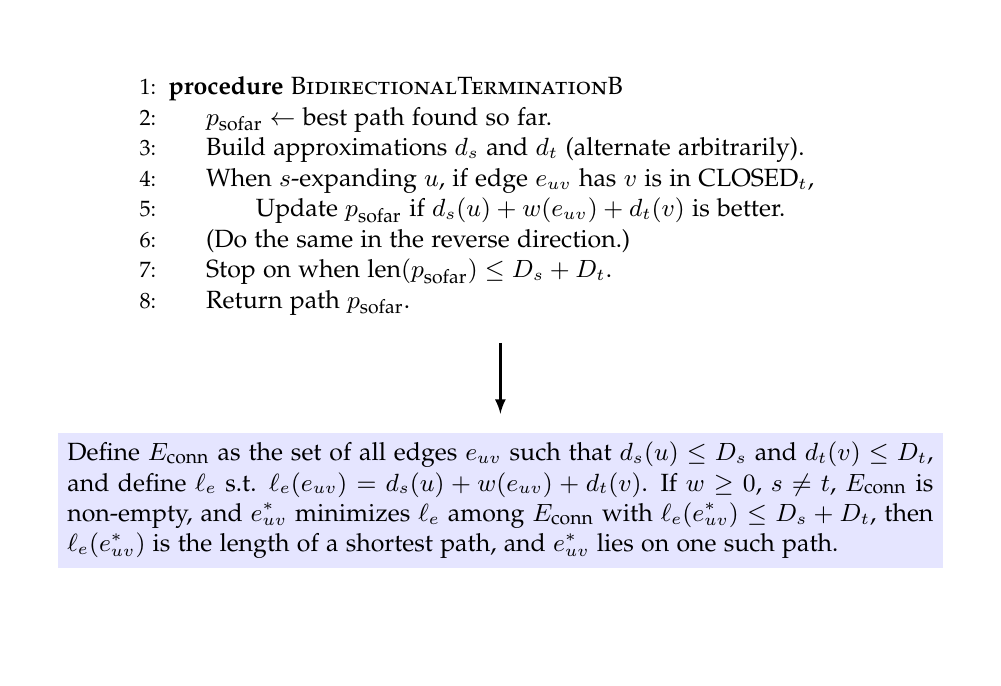
\begin{tikzpicture}[font=\small]
      \tikzset{>=latex} % arrow heads
      \draw[step=1,black!15,very thin,opacity=\gridopacity] (0,0) grid (12,8);

      \node[anchor=north] at (6,7.5) {\begin{minipage}{9.5cm}
         \definecolor{greenhighlight}{rgb}{0.8, 1.0, 0.8}
         \begin{algorithmic}[1]
         \Procedure{BidirectionalTerminationB}{}
         \State $p_{\ms{sofar}} \leftarrow$ best path found so far.
         \State Build approximations $d_s$ and $d_t$ (alternate arbitrarily).
         \State When $s$-expanding $u$, if edge $e_{uv}$ has $v$ is in CLOSED$_t$,
         \State \qquad Update $p_{\ms{sofar}}$ if $d_s(u) + w(e_{uv}) + d_t(v)$ is better.
         \State (Do the same in the reverse direction.)
         \State Stop on when $\mbox{len}(p_{\ms{sofar}}) \leq D_s + D_t$.
         \State Return path $p_{\ms{sofar}}$.
         \EndProcedure
         \end{algorithmic}
      \end{minipage}};

      \only<2>{
      \draw[->,thick] (6,4.0) -- (6,3.1);
      \node[fill=blue!10] at (6,2.0) {\begin{minipage}{11cm}
         Define $E_{\ms{conn}}$ as the set of all edges $e_{uv}$ such that
         $d_s(u) \leq D_s$ and $d_t(v) \leq D_t$,
         and define $\ell_e$ s.t. $\ell_e(e_{uv}) = d_s(u) + w(e_{uv}) + d_t(v)$.
         If $w \geq 0$,
         $s \neq t$,
         $E_{\ms{conn}}$ is non-empty,
         and $e^*_{uv}$ minimizes $\ell_e$
         among $E_{\ms{conn}}$ with $\ell_e(e^*_{uv}) \leq D_s + D_t$,
         then $\ell_e(e^*_{uv})$ is the length of a shortest path,
         and $e^*_{uv}$ lies on one such path.
      \end{minipage}};
      }
      
   \end{tikzpicture}
\end{frame}

\begin{frame}
   \frametitle{Outline of Selected Algorithms}
   \begin{tikzpicture}[font=\small]
      \tikzset{>=latex} % arrow heads
      \draw[step=1,black!15,very thin,opacity=\gridopacity] (0,0) grid (12,8);

      \node[inner sep=0pt,anchor=north] at (6,7.0) {\begin{minipage}{9.05cm}
         \begin{tabular}{ccc}
            \toprule
            & Non-Incremental & Incremental \\
            \midrule
            \addlinespace[0.2em]
            \strut Unidirectional
               & Dijkstra's Algorithm
               & DynamicSWSF-FP \\
            \addlinespace[-0.2em]
            \strut {\color{gray}\emph{(Heuristic)}}
               & {\color{gray}\emph{A*}}
               & {\color{gray}\emph{Lifelong Planning A*}} \\
            \addlinespace[0.3em]
            \strut Bidirectional
               & Bidirectional Dijkstra
               & \only<1>{\multirow{2}{*}{\large\color{gray}?}}
                 \only<2>{IBiD} \\
            \addlinespace[-0.2em]
            \strut {\color{gray}\emph{(Heuristic)}}
               & {\color{gray}\emph{Bidirectional A*}}
               & \only<2>{\color{gray}?} \\
            \addlinespace[0.2em]
            \bottomrule
         \end{tabular}
      \end{minipage}};

      \node[fill=blue!5,draw=blue!15,rounded corners] at (6,4) {\begin{minipage}{10cm}Key Insights:\end{minipage}};

      \node[fill=black!5,draw=black!15,rounded corners,
         anchor=north,minimum width=3.0cm,minimum height=2.5cm] (trustblock) at (2.5,3.6) {};
      \node[fill=white,rounded corners,inner sep=2pt,below=0.1cm of trustblock.north]
         {\includegraphics[height=1.7cm]{build/ibid-dijkstra-trust-build,winctrust}};
      \node[align=center,font=\footnotesize,anchor=south] at (trustblock.south) {Trust Regions};

      \node[fill=black!5,draw=black!15,rounded corners,
         anchor=north,minimum width=3.0cm,minimum height=2.5cm] (termblock) at (6.0,3.6) {};
      \node[fill=white,rounded corners,inner sep=2pt,below=0.1cm of termblock.north]
         {\includegraphics[height=1.5cm]{build/ibid-bidijkstra-viz-build,e}};
      \node[align=center,font=\footnotesize,anchor=south] at (termblock.south) {Bidirectional\\Termination};

      \node[fill=black!5,draw=black!15,rounded corners,
         anchor=north,minimum width=3.0cm,minimum height=2.5cm] (potblock) at (9.5,3.6) {};
      \node[fill=white,rounded corners,inner sep=2pt,below=0.1cm of potblock.north]
         {\includegraphics[height=1.5cm]{build/ibid-potentials}};
      \node[align=center,font=\footnotesize,anchor=south] at (potblock.south) {Potential\\Functions};

   \end{tikzpicture}
\end{frame}

\begin{frame}
   \frametitle{Incremental Bidirectional Dijkatra's Algorithm (IBiD)}
   \begin{tikzpicture}[font=\small]
      \tikzset{>=latex} % arrow heads
      \draw[step=1,black!15,very thin,opacity=\gridopacity] (0,0) grid (12,8);

      \only<2->{
      \node[fill=black!5,draw=black!15,rounded corners,
         minimum width=3.0cm,minimum height=2.5cm] (trustblock) at (2.6,6.5) {};
      \node[fill=white,rounded corners,inner sep=2pt,below=0.1cm of trustblock.north]
         {\includegraphics[height=1.7cm]{build/ibid-dijkstra-trust-build,winctrust}};
      \node[align=center,font=\footnotesize,anchor=south] at (trustblock.south) {Trust Regions};

      \node[fill=black!5,draw=black!15,rounded corners,
         minimum width=3.0cm,minimum height=2.5cm] (termblock) at (9.4,6.5) {};
      \node[fill=white,rounded corners,inner sep=2pt,below=0.1cm of termblock.north]
         {\includegraphics[height=1.5cm]{build/ibid-bidijkstra-viz-build,e}};
      \node[align=center,font=\footnotesize,anchor=south] at (termblock.south) {Bidirectional\\Termination};
      }

      \node[anchor=north,inner sep=0pt] at (6,4.5) {\includegraphics[width=5.5cm]{build/ibid-bidijkstra-sep}};

      \node[fill=blue!10,draw=blue!40!black,rounded corners,align=center,minimum width=3.1cm,anchor=north] at (1.6,4.5) {$Q_s$: $d_s$ Inconsistent\\Vertex Queue\\(DynamicSWSF-FP)};

      \node[fill=red!10,draw=red!40!black,rounded corners,align=center,minimum width=3.1cm,anchor=north] at (10.4,4.5) {$Q_t$: $d_t$ Inconsistent\\Vertex Queue\\(DynamicSWSF-FP)};

      \only<3->{
         \node[fill=green!20,draw=green!40!black,rounded corners,align=center] (connblock) at (6,5.3) {$Q_c$: Connection\\Edge Queue};
         \draw[->,thick] (trustblock) -- (connblock);
         \draw[->,thick] (termblock) -- (connblock);
      }

      \only<4->{
         \node[fill=black!5,draw=black!15,rounded corners] at (6,0.7) {Given $w > 0$, IBiD is {\bf complete} and {\bf optimal}.};
      }

   \end{tikzpicture}
\end{frame}

\begin{frame}
   \frametitle{Traffic Problem Results}
   \begin{tikzpicture}[font=\small]
      \tikzset{>=latex} % arrow heads
      \draw[step=1,black!15,very thin,opacity=\gridopacity] (0,0) grid (12,8);

      \node at (3.2,6.4) {\begin{minipage}{6.1cm}
         9th DIMACS Implementation Challenge

         $G$: 1,524,453 vertices and 3,868,020 edges

         \vspace{0.15cm}
         Traffic model:
         \vspace{-0.1cm}
         \begin{itemize}
         \setlength\itemsep{-0.05cm}
         \item Independently blocked edges
         \item $P_{\ms{blocked}} = 0.002$
         \item Transitions: $P_{\ms{block}}: 0.0010 \mbox{ to } 0.0001$
         \item 10 planning episodes
         \end{itemize}
      \end{minipage}};

      \node[draw=black!30,inner sep=0pt] (exdijk) at (1.7,3.7) {
         \includegraphics[width=3cm]{figs/incbi-road-ne/singleshot/example-dijkstra.png}};
      \node[draw=black!30,inner sep=0pt] (exdynswsf) at (4.8,3.7) {
         \includegraphics[width=3cm]{figs/incbi-road-ne/singleshot/example-incuni-1.png}};
         
      \node[draw=black!30,inner sep=0pt] (exbidijk) at (1.7,1.3) {
         \includegraphics[width=3cm]{figs/incbi-road-ne/singleshot/example-bidijkstra.png}};
      \node[draw=black!30,inner sep=0pt] (exibid) at (4.8,1.3) {
         \includegraphics[width=3cm]{figs/incbi-road-ne/singleshot/example-incbi-1.png}};

      \node[anchor=south east] at (exdijk.south east) {Dijk};
      \node[anchor=south east] at (exdynswsf.south east) {DynSWSF};
      \node[anchor=south east] at (exbidijk.south east) {BiDijk};
      \node[anchor=south east] at (exibid.south east) {IBiD};

      \node at (9.2,3.8) {\includegraphics{build/incbi-road-ne/stats2vert-nonheur}};

   \end{tikzpicture}
\end{frame}

\begin{frame}
   \frametitle{Outline of Selected Algorithms}
   \begin{tikzpicture}[font=\small]
      \tikzset{>=latex} % arrow heads
      \draw[step=1,black!15,very thin,opacity=\gridopacity] (0,0) grid (12,8);

      \node[inner sep=0pt,anchor=north] at (6,7.0) {\begin{minipage}{9.05cm}
         \begin{tabular}{ccc}
            \toprule
            & Non-Incremental & Incremental \\
            \midrule
            \addlinespace[0.2em]
            \strut Unidirectional
               & Dijkstra's Algorithm
               & DynamicSWSF-FP \\
            \addlinespace[-0.2em]
            \strut {\only<1>{\color{gray}}\emph{(Heuristic)}}
               & {\only<1>{\color{gray}}\emph{A*}}
               & {\only<1>{\color{gray}}\emph{Lifelong Planning A*}} \\
            \addlinespace[0.3em]
            \strut Bidirectional
               & Bidirectional Dijkstra
               & IBiD \\
            \addlinespace[-0.2em]
            \strut {\only<1>{\color{gray}}\emph{(Heuristic)}}
               & {\only<1>{\color{gray}}\emph{Bidirectional A*}}
               & \only<1>{\color{gray}?}
                 \only<2->{\emph{Heuristic IBiD}} \\
            \addlinespace[0.2em]
            \bottomrule
         \end{tabular}
      \end{minipage}};

      \node[fill=blue!5,draw=blue!15,rounded corners] at (6,4) {\begin{minipage}{10cm}Key Insights:\end{minipage}};

      \node[fill=black!5,draw=black!15,rounded corners,
         anchor=north,minimum width=3.0cm,minimum height=2.5cm] (trustblock) at (2.5,3.6) {};
      \node[fill=white,rounded corners,inner sep=2pt,below=0.1cm of trustblock.north]
         {\includegraphics[height=1.7cm]{build/ibid-dijkstra-trust-build,winctrust}};
      \node[align=center,font=\footnotesize,anchor=south] at (trustblock.south) {Trust Regions};

      \node[fill=black!5,draw=black!15,rounded corners,
         anchor=north,minimum width=3.0cm,minimum height=2.5cm] (termblock) at (6.0,3.6) {};
      \node[fill=white,rounded corners,inner sep=2pt,below=0.1cm of termblock.north]
         {\includegraphics[height=1.5cm]{build/ibid-bidijkstra-viz-build,e}};
      \node[align=center,font=\footnotesize,anchor=south] at (termblock.south) {Bidirectional\\Termination};

      \node[fill=black!5,draw=black!15,rounded corners,
         anchor=north,minimum width=3.0cm,minimum height=2.5cm] (potblock) at (9.5,3.6) {};
      \node[fill=white,rounded corners,inner sep=2pt,below=0.1cm of potblock.north]
         {\includegraphics[height=1.5cm]{build/ibid-potentials}};
      \node[align=center,font=\footnotesize,anchor=south] at (potblock.south) {Potential\\Functions};

      \only<2>{
         \draw[thick,rounded corners] (potblock.south west) rectangle (potblock.north east);
      }

   \end{tikzpicture}
\end{frame}

\begin{frame}
   \frametitle{Heuristics as Vertex Potential Functions}
   \begin{tikzpicture}[font=\small]
   \tikzset{>=latex} % arrow heads
   \draw[step=1,black!15,very thin,opacity=\gridopacity] (0,0) grid (12,8);

   \begin{scope}[shift={(0.2,2.5)}]
   \node at (2.4,4.1) {Directed graph $G = (V,E)$};
   
   % vertices
   \node[fill=black,circle,inner sep=1.3pt] (s) at (1.8,2.0) {};
   \node[fill=black,circle,inner sep=1.3pt] (a) at (2.9,2.9) {};
   \node[fill=black,circle,inner sep=1.3pt] (b) at (3.6,1.2) {};
   \node[fill=black,circle,inner sep=1.3pt] (c) at (2.7,1.7) {};
   \node[fill=black,circle,inner sep=1.3pt] (d) at (1.2,3.6) {};
   \node[fill=black,circle,inner sep=1.3pt] (e) at (1.9,3.1) {};
   \node[fill=black,circle,inner sep=1.3pt] (f) at (3.5,2.0) {}; % frontier
   \node[fill=black,circle,inner sep=1.3pt] (g) at (1.1,2.7) {};
   \node[fill=black,circle,inner sep=1.3pt] (h) at (0.3,3.6) {};
   \node[fill=black,circle,inner sep=1.3pt] (i) at (0.2,2.83) {};
   \node[fill=black,circle,inner sep=1.3pt] (j) at (0.5,2.0) {};
   \node[fill=black,circle,inner sep=1.3pt] (k) at (1.2,1.5) {};
   \node[fill=black,circle,inner sep=1.3pt] (l) at (2.2,1.1) {};
   \node[fill=black,circle,inner sep=1.3pt] (m) at (1.42,0.5) {};
   \node[fill=black,circle,inner sep=1.3pt] (n) at (0.5,0.8) {};
   \node[fill=black,circle,inner sep=1.3pt] (o) at (3.0,0.6) {};
   \node[fill=black,circle,inner sep=1.3pt] (p) at (4.0,0.3) {};
   \node[fill=black,circle,inner sep=1.3pt] (q) at (4.7,0.9) {};
   \node[fill=black,circle,inner sep=1.3pt] (r) at (4.3,1.7) {};
   \node[fill=black,circle,inner sep=1.3pt] (t) at (4.1,2.9) {};
   \node[fill=black,circle,inner sep=1.3pt] (u) at (3.5,3.6) {};
   \node[fill=black,circle,inner sep=1.3pt] (v) at (0.6,0.2) {};

   \draw[->,draw=black!50] (s) -- (c);
   \draw[->,draw=black!50] (s) -- (e);
   \draw[->,draw=black!50] (e) -- (a);
   \draw[->,draw=black!50] (g) -- (e);
   \draw[->,draw=black!50] (e) -- (d);
   \draw[->,draw=black!50] (a) -- (f);
   \draw[->,draw=black!50] (g) -- (j);
   \draw[->,draw=black!50] (g) -- (d);
   \draw[->,draw=black!50] (d) -- (h);
   \draw[->,draw=black!50] (i) -- (h);
   \draw[->,draw=black!50] (g) -- (i);
   \draw[->,draw=black!50] (j) -- (i);
   \draw[->,draw=black!50] (s) -- (g);
   \draw[->,draw=black!50] (k) -- (j);
   \draw[->,draw=black!50] (k) -- (l);
   \draw[->,draw=black!50] (k) -- (n);
   \draw[->,draw=black!50] (j) -- (n);
   \draw[->,draw=black!50] (m) -- (n);
   \draw[->,draw=black!50] (s) -- (j);
   \draw[->,draw=black!50] (s) -- (k);
   \draw[->,draw=black!50] (k) -- (m);
   \draw[->,draw=black!50] (s) -- (l);
   \draw[->,draw=black!50] (l) -- (m);
   \draw[->,draw=black!50] (c) -- (l);
   \draw[->,draw=black!50] (l) -- (o);
   \draw[->,draw=black!50] (o) -- (p);
   \draw[->,draw=black!50] (o) -- (b);
   \draw[->,draw=black!50] (b) -- (p);
   \draw[->,draw=black!50] (b) -- (f);
   \draw[->,draw=black!50] (c) -- (f);
   \draw[->,draw=black!50] (p) -- (q);
   \draw[->,draw=black!50] (b) -- (r);
   \draw[->,draw=black!50] (f) -- (r);
   \draw[->,draw=black!50] (r) -- (q);
   \draw[->,draw=black!50] (f) -- (t);
   \draw[->,draw=black!50] (a) -- (t);
   \draw[->,draw=black!50] (a) -- (u);
   \draw[->,draw=black!50] (u) -- (t);
   \draw[->,draw=black!50] (n) -- (v);
   \end{scope}

   \node[fill=black!3,rounded corners,align=center] (blocka) at (7.3,6.6) {
      \strut $w : E \rightarrow \mathbb{R}$};

   \only<2->{
   \node[fill=black!3,rounded corners,align=center] (blockb) at (7.3,5.5) {
      Vertex potential:\\
      \strut $b : V \rightarrow \mathbb{R}$};
   }

   \only<3->{
   \node[fill=black!3,rounded corners,align=center] (blockc) at (7.3,4.2) {
      \strut $w' : E \rightarrow \mathbb{R}$\\
      \strut $w'_{uv} = w_{uv} - \left( b(u)\!-\!b(v) \right)$};
   }

   \only<4->{
   \node[fill=blue!5,rounded corners,align=center] at (8.5,1.8) {
      $\arraycolsep=1.5pt \begin{array}{rl}
         \vspace{0.1cm}
         \mbox{len}(p_{st}, w') = & w'_{su} + w'_{uv} \dots \\
          = & w_{su} - \left( b(s)\!-\!b(u) \right) \\
          & + \; w_{su} - \left( b(u)\!-\!b(v) \right) \\
          & + \; \dots \vspace{0.1cm} \\
          = & \mbox{len}(p_{st}, w) - \left( b(s)\!-\!b(t) \right)
      \end{array}$\\
      \vspace{0.0cm}\\
      Length difference independent of $p_{st}$!};
   }

   \only<5->{
   \node[fill=blue!5,rounded corners,align=center] (blockd) at (10.7,4.2) {
      Shortest path\\ \strut $p'_{st}$ w.r.t. $w'$};
   }

   \only<6->{
   \node[fill=blue!5,rounded corners,align=center] (blocke) at (10.7,6.6) {
      Shortest path\\ \strut $p_{st}$ w.r.t. $w$};
   }

   \only<7->{\draw[->] (blocka) -- (blockb);}
   \only<8->{\draw[->] (blockb) -- (blockc);}
   \only<9->{\draw[->] (blockc) -- (blockd);}
   \only<10->{\draw[->] (blockd) -- (blocke);}
   

   \end{tikzpicture}
\end{frame}

\begin{frame}
   \frametitle{Heuristics as Vertex Potential Functions}
   \begin{tikzpicture}[font=\small]
   \tikzset{>=latex} % arrow heads
   \draw[step=1,black!15,very thin,opacity=\gridopacity] (0,0) grid (12,8);

   \node[fill=black!3,minimum width=5.2cm] at (3.7,7.55) {\strut Non-Incremental};
   \node[fill=black!3,minimum width=3.3cm,rotate=90] at (0.6,5.45) {\strut Unidirectional};
   \only<6->{\node[fill=black!3,minimum width=5.2cm] at (9.0,7.55) {\strut Incremental};}
   \only<17->{\node[fill=black!3,minimum width=3.45cm,rotate=90] at (0.6,1.85) {\strut Bidirectional};}

   \only<2->{
   \node[fill=blue!5,rounded corners,anchor=north,minimum width=5cm,minimum height=3.3cm] (dijk) at (3.7,7.1) {};
   \node[anchor=north] at (dijk.north) {\begin{minipage}{4.7cm}
      \setlength{\belowdisplayskip}{1pt} \setlength{\belowdisplayshortskip}{1pt}
      \setlength{\abovedisplayskip}{1pt} \setlength{\abovedisplayshortskip}{1pt}

      Use potential function:
      \[
         b(v) = h_t(v)
      \]
      \[
         w'_{uv} = w_{uv} - \left( b(u)\!-\!b(v) \right) 
      \]
      
      \only<5->{
      \vspace{0.7cm}
      \begin{center}
         Dijkstra's algorithm on $w'$\\
         yields A*
      \end{center}}
   \end{minipage}};
   }
   \only<3->{\node[fill=blue!10,rounded corners,inner sep=3pt,align=center] (dijkin) at (2.7,5.2) {$w \geq 0$\\$h_t$ consistent};}
   \only<4->{
      \node[fill=blue!10,rounded corners,inner sep=3pt] (dijkout) at (5.2,5.2) {$w_{uv}' \geq 0$};
      \draw[->] (dijkin) -- (dijkout);}


   \only<7->{
   \node[fill=blue!5,rounded corners,anchor=north,minimum width=5cm,minimum height=3.3cm] (dynswsffp) at (9.0,7.1) {};
   \only<24->{
      \node[fill=green!20,anchor=north,minimum width=5cm,minimum height=0.55cm,below=0.85cm of dynswsffp.north]  {};
   }
   \node[anchor=north] at (dynswsffp.north) {\begin{minipage}{4.7cm}
      \setlength{\belowdisplayskip}{1pt} \setlength{\belowdisplayshortskip}{1pt}
      \setlength{\abovedisplayskip}{1pt} \setlength{\abovedisplayshortskip}{1pt}
      \only<8->{
      Use potential function:
      \[
         b(v) = h_t(v)
      \]}%
      \only<9-11>{\[
         w'_{uv} = w_{uv} - \left( b(u)\!-\!b(v) \right)
      \]}%
      \only<13-15>{\[
         w'_{uv} = \left[ w_{uv} - \left( b(u)\!-\!b(v) \right), \;\;\, ? \;\;\; \right]
      \]}%
      \only<16->{\[
         w'_{uv} = \left[ w_{uv} - \left( b(u)\!-\!b(v) \right), \; w_{uv} \right]
      \]}%
      
      \only<15->{%
      \vspace{0.7cm}
      \begin{center}
         DynamicSWSF-FP on $w'$\\
         yields LPA*
      \end{center}%
      }
   \end{minipage}};
   }
   \only<10->{\node[fill=blue!10,rounded corners,inner sep=3pt,align=center] (dynswsffpin) at (8.0,5.2) {$w_{uv} > 0$\\$h_t$ consistent};}
   \only<11>{
      \node[fill=blue!10,rounded corners,inner sep=3pt] (dynswsffpout) at (10.5,5.2) {$w_{uv}' \ngtr 0$};
      \draw[->] (dynswsffpin) -- (dynswsffpout);}
   \only<14->{
      \node[fill=blue!10,rounded corners,inner sep=3pt] (dynswsffpout) at (10.5,5.2) {$w_{uv}' > [0,0]$};
      \draw[->] (dynswsffpin) -- (dynswsffpout);}


   \only<18->{
   \node[fill=blue!5,rounded corners,anchor=north,minimum width=5cm,minimum height=3.5cm] (bidijk) at (3.7,3.6) {};
   \only<22->{
      \node[fill=green!20,anchor=north,minimum width=5cm,minimum height=0.55cm,below=0.45cm of bidijk.north]  {};
   }
   \node[anchor=north] at (bidijk.north) {\begin{minipage}{4.7cm}
      \setlength{\belowdisplayskip}{2pt} \setlength{\belowdisplayshortskip}{2pt}
      \setlength{\abovedisplayskip}{2pt} \setlength{\abovedisplayshortskip}{2pt}

      Use potential function:
      \[
         b(v) = \tfrac{1}{2} h_t(v) - \tfrac{1}{2} h_s(v)
      \]
      \[
         w'_{uv} = w_{uv} - \left( b(u)\!-\!b(v) \right) 
      \]

      \vspace{0.7cm}
      \begin{center}
         Bidirectional Dijkstra's on $w'$\\
         yields Bidirectional A*
      \end{center}
   \end{minipage}};
   }
   \only<18>{
      \node[fill=blue!5,anchor=north,rounded corners,minimum width=5cm,minimum height=1.0cm,below=0.0cm of bidijk.north] {};
   }
   \only<18-19>{
      \node[fill=blue!10,rounded corners,inner sep=3pt,align=center] (bidijkin) at (2.7,1.6) {$w \geq 0$\\ \strut $b$ consistent};
   }
   \only<20->{
      \node[fill=blue!10,rounded corners,inner sep=3pt,align=center] (bidijkin) at (2.7,1.6) {$w \geq 0$\\ \strut $h_s, h_t$ consistent};
   }
   \only<18->{
      \node[fill=blue!10,rounded corners,inner sep=3pt] (bidijkout) at (5.2,1.6) {$w' \geq 0$};
      \draw[->] (bidijkin) -- (bidijkout);
   }


   \only<21->{
   \node[fill=blue!5,rounded corners,anchor=north,minimum width=5cm,minimum height=3.5cm] (ibid) at (9.0,3.6) {};
   \only<23-24>{
      \node[fill=green!20,anchor=north,minimum width=5cm,minimum height=0.55cm,below=0.45cm of ibid.north]  {};
   }
   \only<25->{
      \node[fill=green!20,anchor=north,minimum width=5cm,minimum height=1.05cm,below=0.45cm of ibid.north]  {};
   }
   \node[anchor=north] at (ibid.north) {\begin{minipage}{4.7cm}
      \setlength{\belowdisplayskip}{2pt} \setlength{\belowdisplayshortskip}{2pt}
      \setlength{\abovedisplayskip}{2pt} \setlength{\abovedisplayshortskip}{2pt}
      \only<23->{
      Use potential function:
      \[
         b(v) = \tfrac{1}{2} h_t(v) - \tfrac{1}{2} h_s(v)
      \]}%
      \only<25->{\[
         w'_{uv} = \left[ w_{uv} - \left( b(u)\!-\!b(v) \right), \; w_{uv} \right]
      \]}%
      \only<26->{%
      \vspace{0.38cm}
      \begin{center}
         IBiD on $w'$\\
         yields Heuristic IBiD
      \end{center}
      }
   \end{minipage}};
   }
   \only<26->{
   \node[fill=blue!10,rounded corners,inner sep=3pt,align=center] (ibidin) at (8.0,1.6) {$w_{uv} > 0$\\$h_s, h_t$ consistent};
   \node[fill=blue!10,rounded corners,inner sep=3pt] (ibidout) at (10.5,1.6) {$w_{uv}' > [0,0]$};
   \draw[->] (ibidin) -- (ibidout);
   }
   

   \end{tikzpicture}
\end{frame}

\begin{frame}
   \frametitle{Traffic Problem Results: With Euclidean Heuristic}
   \begin{tikzpicture}[font=\small]
      \tikzset{>=latex} % arrow heads
      \draw[step=1,black!15,very thin,opacity=\gridopacity] (0,0) grid (12,8);

      \node at (6,3.8) {\includegraphics{build/incbi-road-ne/stats2vert}};

   \end{tikzpicture}
\end{frame}

\begin{frame}
   \frametitle{Experiment: Traffic Problem}
   \begin{tikzpicture}[font=\small]
      \draw[step=1,black!15,very thin,opacity=\gridopacity] (0,0) grid (12,8);
      
      \node[inner sep=0pt] (vidnode) at (6,4.0) {%
         \href{\tikzvidtarget{incbi-roadne}}{%
         \includegraphics[width=11cm]{videos/incbi-roadne.png}}};
      \tikzvidplayat{incbi-roadne}{vidnode}{videos/incbi-roadne.mp4}{}

   \end{tikzpicture}
\end{frame}

\begin{frame}
   \frametitle{LazySP Problem: Dynamic SP Algorithms}
   \begin{tikzpicture}[font=\small]
      \draw[step=1,black!15,very thin,opacity=\gridopacity] (0,0) grid (12,8);

      \node at (6,4) {\includegraphics{build/ibid-lazysp-plot}};

      %\node[draw=black,inner sep=0pt,thick] at (5.35,6.235) {\includegraphics[width=2.0cm]{figs/herbarm-traj2-t031.png}};
      \node[draw=black,inner sep=0pt,thick,anchor=north] at (5.15,7.325) {\includegraphics[width=2.0cm]{figs/herbarm-traj2-t031.png}};
      \node[draw=black,fill=black!2,anchor=north] at (7.8,7.325) {\strut $h_w = (1 - \lambda) \, h_x$};

   \end{tikzpicture}
\end{frame}


\begin{frame}
   \frametitle{Outline of Selected Algorithms}
   \begin{tikzpicture}[font=\small]
      \tikzset{>=latex} % arrow heads
      \draw[step=1,black!15,very thin,opacity=\gridopacity] (0,0) grid (12,8);

      \node[inner sep=0pt,anchor=north] at (6,7.0) {\begin{minipage}{9.05cm}
         \begin{tabular}{ccc}
            \toprule
            & Non-Incremental & Incremental \\
            \midrule
            \addlinespace[0.2em]
            \strut Unidirectional
               & Dijkstra's Algorithm
               & DynamicSWSF-FP \\
            \addlinespace[-0.2em]
            \strut \emph{(Heuristic)}
               & \emph{A*}
               & \emph{Lifelong Planning A*} \\
            \addlinespace[0.3em]
            \strut Bidirectional
               & Bidirectional Dijkstra
               & IBiD \\
            \addlinespace[-0.2em]
            \strut \emph{(Heuristic)}
               & \emph{Bidirectional A*}
               & \emph{Heuristic IBiD} \\
            \addlinespace[0.2em]
            \bottomrule
         \end{tabular}
      \end{minipage}};

      \node[fill=blue!5,draw=blue!15,rounded corners] at (6,4) {\begin{minipage}{10cm}Key Insights:\end{minipage}};

      \node[fill=black!5,draw=black!15,rounded corners,
         anchor=north,minimum width=3.0cm,minimum height=2.5cm] (trustblock) at (2.5,3.6) {};
      \node[fill=white,rounded corners,inner sep=2pt,below=0.1cm of trustblock.north]
         {\includegraphics[height=1.7cm]{build/ibid-dijkstra-trust-build,winctrust}};
      \node[align=center,font=\footnotesize,anchor=south] at (trustblock.south) {Trust Regions};

      \node[fill=black!5,draw=black!15,rounded corners,
         anchor=north,minimum width=3.0cm,minimum height=2.5cm] (termblock) at (6.0,3.6) {};
      \node[fill=white,rounded corners,inner sep=2pt,below=0.1cm of termblock.north]
         {\includegraphics[height=1.5cm]{build/ibid-bidijkstra-viz-build,e}};
      \node[align=center,font=\footnotesize,anchor=south] at (termblock.south) {Bidirectional\\Termination};

      \node[fill=black!5,draw=black!15,rounded corners,
         anchor=north,minimum width=3.0cm,minimum height=2.5cm] (potblock) at (9.5,3.6) {};
      \node[fill=white,rounded corners,inner sep=2pt,below=0.1cm of potblock.north]
         {\includegraphics[height=1.5cm]{build/ibid-potentials}};
      \node[align=center,font=\footnotesize,anchor=south] at (potblock.south) {Potential\\Functions};

   \end{tikzpicture}
\end{frame}



\begin{frame}
   \frametitle{Lazily Evaluated Marginal Utility Roadmaps}
   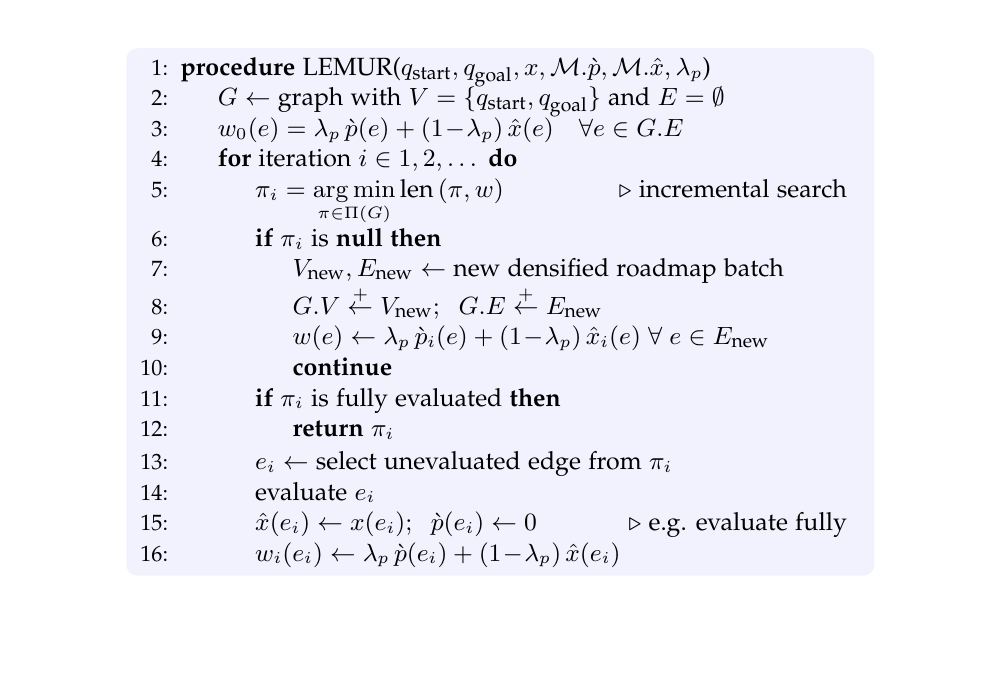
\begin{tikzpicture}[font=\small]
   \draw[step=1,black!15,very thin,opacity=\gridopacity] (0,0) grid (12,8);
   \tikzset{>=latex} % arrow heads

      \node[fill=blue!5,rounded corners,anchor=north,minimum width=9.5cm,minimum height=6.7cm] (alg) at (6,7.75) {};
      \node[left=0.1cm of alg.north,anchor=north] {\begin{minipage}{9cm}
         \begin{algorithmic}[1]
         \Procedure {LEMUR}{$q_{\ms{start}}, q_{\ms{goal}}, x,
            \mathcal{M}.\grave{p}, \mathcal{M}.\hat{x}, \lambda_p$}
         \State $G \leftarrow$ graph with
            $V = \{ q_{\ms{start}}, q_{\ms{goal}} \}$
            and $E = \emptyset$
         %\State $w_0 : E \rightarrow \mathbb{R}^{+}$ \Comment mutable edge weight function
         \State $w_0(e) = \lambda_p \, \grave{p}(e) + (1\!-\!\lambda_p) \, \hat{x}(e) \quad \forall e \in G.E$
         \For {iteration $i \in 1, 2, \dots$}
            \State $\pi_i = \displaystyle\argmin_{\pi \in \Pi(G)} 
               \mbox{len}\left(\pi, w\right)$
               \Comment incremental search
            \If {$\pi_i$ is {\bf null}}
               \State $V_{\ms{new}}, E_{\ms{new}} \leftarrow$ new densified roadmap batch
               \State $G.V \stackrel{\tiny +}\leftarrow V_{\ms{new}};
                  \;\; G.E \stackrel{\tiny +}\leftarrow E_{\ms{new}}$
               \State $w(e) \leftarrow \lambda_p \, \grave{p}_i(e) + (1\!-\!\lambda_p) \, \hat{x}_i(e)
                  \; \forall \; e \in E_{\ms{new}}$
               \State {\bf continue}
            \EndIf
            \If {$\pi_i$ is fully evaluated}
               \State \Return $\pi_i$
            \EndIf
            \State $e_i \leftarrow$ select unevaluated edge from $\pi_i$
            \State evaluate $e_i$
            \State $\hat{x}(e_i) \leftarrow x(e_i); \;\; \grave{p}(e_i) \leftarrow 0$
               \Comment e.g. evaluate fully
            \State $w_i(e_i) \leftarrow
               \lambda_p \, \grave{p}(e_i) + (1\!-\!\lambda_p) \, \hat{x}(e_i)$
         \EndFor
         \EndProcedure
         \end{algorithmic}
      \end{minipage}};


   \end{tikzpicture}
\end{frame}

\begin{frame}
   \frametitle{Maximizing Utility: HERB Bin Experiments}
   \begin{tikzpicture}[font=\small]
      \tikzset{>=latex} % arrow heads
      \draw[step=1,black!15,very thin,opacity=\gridopacity] (0,0) grid (12,8);

      \node at ( 3.75,6.4) {
         \includegraphics[width=1.7cm]{figs/herbbin/step0cropped.png}
         \;\includegraphics[width=1.7cm]{figs/herbbin/step01cropped.png}};

      %\node[inner sep=0pt] (vidnode) at (9.5,6.5) {%
      %   \href{\tikzvidtarget{incbi-roadne}}{%
      %   \includegraphics[width=4cm]{videos/workcell-cropped.png}}};
      %\tikzvidplayat{incbi-roadne}{vidnode}{videos/workcell-cropped.mp4}{}

      \node at (3.5,2.5) {\includegraphics[width=7cm]{build/lemur-sq/herbbin0}};

      \node at (9.5,2.5) {\includegraphics[height=4cm]{build/multistep-prescribed/herbbinnom-g1ll-lemuronly}};
      
   \end{tikzpicture}
\end{frame}

\begin{frame}
   \frametitle{Maximizing Utility: Workcell Experiments}
   \begin{tikzpicture}[font=\small]
      \tikzset{>=latex} % arrow heads
      \draw[step=1,black!15,very thin,opacity=\gridopacity] (0,0) grid (12,8);

      \node at ( 3.75,6.4) {
         \includegraphics[width=2.7cm]{figs/workcell/cropped-config-f.png}
         \;\includegraphics[width=2.7cm]{figs/workcell/cropped-config-g.png}};

      \node[inner sep=0pt] (vidnode) at (9.5,6.5) {%
         \href{\tikzvidtarget{workcell-cropped}}{%
         \includegraphics[width=4cm]{videos/workcell-cropped.png}}};
      \tikzvidplayat{workcell-cropped}{vidnode}{videos/workcell-cropped.mp4}{}

      \node at (3.5,2.5) {\includegraphics[width=7cm]{build/lemur-sq/workcellfg}};

      \node at (9.5,2.5) {\includegraphics[height=4cm]{build/multistep-prescribed/workcell-g1ll-lemuronly}};
      
   \end{tikzpicture}
\end{frame}



\begin{frame}
   \frametitle{Planning over C-Space Families}
   \begin{tikzpicture}[font=\small]
   \tikzset{>=latex} % arrow heads
   \draw[step=1,black!15,very thin,opacity=\gridopacity] (0,0) grid (12,8);

   \node[fill=black!2,draw=black!5,rounded corners,minimum height=7.45cm,anchor=north] at (3.5,7.7)
   {\begin{minipage}{4.0cm}
      Structure of joint C-space \dots%
      \vspace{-0.25cm}%
      \begin{center}
         \includegraphics[width=3cm]{build/family-composite/plot-g-manifold}
      \end{center}%
      \vspace{-0.25cm}%
      \dots projected onto $\mathcal{C}_{\ms{robot}}$:%
      \vspace{-0.25cm}%
      \begin{center}
         \includegraphics[width=3cm]{build/multiple-sets}
      \end{center}
   \end{minipage}};

   \node[fill=blue!10,draw=blue!20,rounded corners,align=center,minimum width=5.0cm,minimum height=1.5cm,anchor=north] at (8.5,7.7)
   {$\arraycolsep=1.5pt \begin{array}{cl}
      x(\xi)\!: & \mbox{execution cost} \;(\mathcal{C}_{\ms{free}}) \\
      \hat{x}(\xi)\!: & \mbox{execution cost estimate} \\
      \grave{p}(\xi)\!: & \mbox{planning cost estimate}
   \end{array}$};

   \node[fill=black!2,draw=black!5,rounded corners,minimum width=5.0cm,minimum height=5.75cm,anchor=north] at (8.5,6.0)
   {\begin{minipage}{4.5cm}
      Assign to each roadmap edge $\xi_e$
      a belief state $b_e$
      which captures belief over subset membership:%
      \vspace{-0.2cm}%
      \begin{center}
         \includegraphics[width=3cm]{build/family-belief-graph-example-wrels-policy}
      \end{center}%
      \vspace{-0.2cm}%
      A shortest path from $b_e$ of belief transitions
      yields $\grave{p}(\xi)$.
   \end{minipage}};

   \end{tikzpicture}
\end{frame}


%\begin{frame}
%   \frametitle{Talk Outline}
%   \begin{tikzpicture}[font=\small]
%      \tikzset{>=latex} % arrow heads
%      \draw[step=1,black!15,very thin,opacity=\gridopacity] (0,0) grid (12,8);
%
%      \node[fill=blue!15,minimum width=11cm] at (6,7.5) {\strut How to Optimize?};
%
%      \node[fill=black!3,minimum width=5cm,minimum height=3cm] (lazysp) at (3.25,5.6) {};
%      \node[anchor=north] at (lazysp.north) {\strut Lazy Pathfinding};
%      \node[draw=black!30,fill=white,inner sep=5pt] at (3.25,5.4) {
%         \includegraphics[width=3.8cm]{build/lazysp-icon}};
%
%      \node[fill=black!3,minimum width=5cm,minimum height=3cm] (ibid) at (8.75,5.6) {};
%      \node[anchor=north] at (ibid.north) {\strut Dynamic Pathfinding};
%      \node[draw=black!30,inner sep=0pt] at (8.75,5.4) {
%         \includegraphics[width=2.9cm]{figs/incbi-road-ne/singleshot/example-bidijkstra.png}};
%
%      \node[fill=blue!15,minimum width=11cm] at (6,3.5) {\strut What to Optimize?};
%
%      \node[fill=black!3,minimum width=5cm,minimum height=3cm] (utility) at (3.25,1.6) {};
%      \node[anchor=north] at (utility.north) {\strut Maximizing Utility};
%      \node at (3.25,1.35) {\includegraphics[width=2.5cm]{build/pvx-utility-anytime}};
%
%      \node[fill=black!3,minimum width=5cm,minimum height=3cm] (family) at (8.75,1.6) {};
%      \node[anchor=north] at (family.north) {\strut Utility in C-Space Familes};
%      \node at (8.75,1.4) {\includegraphics[width=3.0cm]{build/multiple-sets}};
%
%      \only<2>
%      {
%      }
%      
%   \end{tikzpicture}
%\end{frame}

%\begin{frame}
%   \frametitle{Planning over C-Space Families}
%   
%\end{frame}

%\begin{frame}
%   \frametitle{Maximizing Utility: HERB Bin Experiments}
%   \begin{tikzpicture}[font=\small]
%      \tikzset{>=latex} % arrow heads
%      \draw[step=1,black!15,very thin,opacity=\gridopacity] (0,0) grid (12,8);
%
%      \node at ( 6,6.5) {
%         \includegraphics[width=1.7cm]{figs/herbbin/step0cropped.png}
%         \;\includegraphics[width=1.7cm]{figs/herbbin/step01cropped.png}};
%
%      \node at ( 6,2.5) {\includegraphics[width=9cm]{build/multistep-prescribed/herbbinnom-g1ll}};
%      
%   \end{tikzpicture}
%\end{frame}

%\begin{frame}
%   \frametitle{Maximizing Utility: Workcell Experiments}
%   \begin{tikzpicture}[font=\small]
%      \tikzset{>=latex} % arrow heads
%      \draw[step=1,black!15,very thin,opacity=\gridopacity] (0,0) grid (12,8);
%
%      %\node at ( 6,6.5) {
%      %   \includegraphics[width=2.7cm]{figs/workcell/cropped-config-f.png}
%      %   \;\includegraphics[width=2.7cm]{figs/workcell/cropped-config-g.png}};
%
%      \node[inner sep=0pt] (vidnode) at (6,6.5) {%
%         \href{\tikzvidtarget{incbi-roadne}}{%
%         \includegraphics[width=4cm]{videos/workcell-cropped.png}}};
%      \tikzvidplayat{incbi-roadne}{vidnode}{videos/workcell-cropped.mp4}{}
%
%      \node at ( 6,2.5) {\includegraphics[height=4cm]{build/multistep-prescribed/workcell-g1ll-lemuronly}};
%      
%   \end{tikzpicture}
%\end{frame}

\begin{frame}
   \frametitle{Maximizing Utility over C-Space Families}
   \begin{tikzpicture}[font=\small]
      \tikzset{>=latex} % arrow heads
      \draw[step=1,black!15,very thin,opacity=\gridopacity] (0,0) grid (12,8);

      %\node[draw=black!40,rounded corners,inner sep=2pt,anchor=north] at ( 3.75,6.4) {
      %   \includegraphics[width=2.7cm]{figs/workcell/cropped-config-f.png}
      %   \;\includegraphics[width=2.7cm]{figs/workcell/cropped-config-g.png}};

      \node[inner sep=0pt] (herbbin-cropped) at (3.5,6.0) {%
         \href{\tikzvidtarget{herbbin-cropped}}{%
         \includegraphics[width=3.5cm]{videos/herbbin-cropped.png}}};
      \tikzvidplayat{herbbin-cropped}{herbbin-cropped}{videos/herbbin-cropped.mp4}{}

      \node[inner sep=0pt] (workcell-cropped) at (8.5,6.0) {%
         \href{\tikzvidtarget{workcell-cropped}}{%
         \includegraphics[width=4cm]{videos/workcell-cropped.png}}};
      \tikzvidplayat{workcell-cropped}{workcell-cropped}{videos/workcell-cropped.mp4}{}

      \node at (3.2,2.2) {\includegraphics[height=4cm]{build/multistep-prescribed/herbbinnom-g1ll-lemuronly}};

      \node at (8.2,2.2) {\includegraphics[height=4cm]{build/multistep-prescribed/workcell-g1ll-lemuronly}};
      
   \end{tikzpicture}
\end{frame}


\begin{frame}
   \frametitle{Summary of Contributions}

   Summary of contributions:
   \begin{itemize}
   \pause \item {\bf LazySP} algorithm for graphs with expensive edge evaluations
   \pause \item {\bf IBiD} algorithm for incremental bidirectional search
   \pause \item {\bf LEMUR} algorithm for motion planning with utility functions
   \pause \item {\bf C-space family decomposition} for multi-step planning tasks
   \end{itemize}

   \pause
   Code is available:
   \begin{itemize}
   \item {\tt http://lemur-planning.readthedocs.io}
   \item {\tt https://github.com/personalrobotics/lemur}
   \end{itemize}

   %Future work?

   %Discussion!

   %Roadmap stacks!
   
\end{frame}

\begin{frame}
   \frametitle{Thank You!}
   \begin{tikzpicture}[font=\small]
   \draw[step=1,black!15,very thin,opacity=\gridopacity] (0,0) grid (12,8);
   \tikzset{>=latex} % arrow heads

   % START LEMUR
   \node[fill=blue!5,draw=blue!10,rounded corners,minimum width=9.7cm,minimum height=5.8cm,anchor=north] (lemur) at (6,6.0) {};
   \node[anchor=north west] at (lemur.north west) {LEMUR};

   % left side

   \node[fill=blue!10,draw=blue!20,rounded corners,align=center,minimum height=1.5cm,minimum width=2.5cm,inner sep=0pt] at (3.3,4.5) {};
   \node at (3.3,4.5) {\includegraphics[width=1.8cm]{build/roadmap-stack-short}};
   \draw[->] (3.3,3.75) -- (3.3,3.0) node [pos=0.45,fill=blue!5,align=center,inner sep=2pt] {$G$};

   % right side

   \node[fill=blue!10,draw=blue!20,rounded corners,align=center,minimum height=1.5cm,inner sep=0pt] at (7.8,4.5) {
      \qquad\qquad\; $ \arraycolsep=1.5pt \begin{array}{rcc}
         w_{\ms{est}}(e) = & \lambda \, \grave{p}(e) \; + & (1\!-\!\lambda) \, \hat{x}(e) \\
         w(e) = & & (1\!-\!\lambda) \, x(e)
      \end{array} $
   };
   %\node[fill=black!3,draw=blue!20,inner sep=2pt] at (7,5.4) {\includegraphics[width=1.3cm]{build/pvx-utility-anytime-simple}};
   \node[fill=black!3,draw=blue!20,inner sep=2pt] at (5.6,4.5) {\includegraphics[width=1.0cm]{build/pvx-linear-discounting-simple}};

   \draw[->] (7.3,3.75) -- (7.3,3.0) node [pos=0.45,fill=blue!5,align=center,inner sep=2pt] {$w$};
   \draw[->] (8.2,3.75) -- (8.2,3.0) node [pos=0.45,fill=blue!5,align=center,inner sep=2pt] {$w_{\ms{est}}$};

   % START LAZYSP
   \node[fill=blue!10,draw=blue!20,rounded corners,minimum width=7cm,minimum height=2.5cm,anchor=north] (lazysp) at (6,3.0) {};
   \node[anchor=north west] at (lazysp.north west) {LazySP};

   \node[fill=blue!20,draw=blue!30,rounded corners,align=center] (dynsp) at (4.3,1.7) {DynamicSP\\(e.g. IBiD)};
   \node[fill=blue!20,draw=blue!30,rounded corners,align=center] (selector) at (7.7,1.7) {Edge Selector\\(e.g. Alternate)};

   \draw[->] (dynsp.south) -- (4.3,0.8) -- (7.7,0.8) -- (selector.south);
   \draw[->] (selector.north) -- (7.7,2.6) -- (4.3,2.6) -- (dynsp.north);

   \node[fill=blue!10,align=center,inner sep=2pt] at (6,2.6)
      {$E_{\ms{changed}}$};

   \node[fill=blue!10,align=center,inner sep=2pt] at (6,0.8)
      {$\pi_{\ms{candidate}}$};
   % END LAZYSP

   % END LEMUR

   % top left side
   \node[fill=blue!10,draw=blue!20,rounded corners,align=center,minimum height=1.5cm,minimum width=1.8cm,inner sep=0pt] at (3.3,7.0) {};
   \node[fill=white,inner sep=0pt] at (3.3,7.0) {\includegraphics[width=1.4cm]{build/c-space-simple}};
   \node[font=\scriptsize] at (2.95,6.7) {$\mathcal{C}_{\mbox{\tiny free}}$};
   \draw[->] (3.3,6.25) -- (3.3,5.25) node [pos=0.55,fill=blue!5,align=center,inner sep=0pt] {\strut $\mathcal{C}$};

   %\node[inner sep=4pt] (cspace) at (3.3,7.0) {$\mathcal{C}$-Space};
   %\draw[->] (cspace) -- (3.3,5.25);
   
   % top right side
   \node[fill=blue!10,draw=blue!20,rounded corners,align=center,minimum height=1.5cm] at (7.9,7)
   {$\arraycolsep=1.5pt \begin{array}{cl}
      x(\xi)\!: & \mbox{execution cost} \;(\mathcal{C}_{\ms{free}}) \\
      \hat{x}(\xi)\!: & \mbox{execution cost estimate} \\
      \grave{p}(\xi)\!: & \mbox{planning cost estimate}
   \end{array}$};
   
   \draw[->] (7.3,6.25) -- (7.3,5.25) node [pos=0.55,fill=blue!5,align=center,inner sep=0pt] {\strut $x$};
   \draw[->] (7.9,6.25) -- (7.9,5.25) node [pos=0.55,fill=blue!5,align=center,inner sep=0pt] {\strut $\hat{x}$};
   \draw[->] (8.5,6.25) -- (8.5,5.25) node [pos=0.55,fill=blue!5,align=center,inner sep=0pt] {\strut $\grave{p}$};

   % left side
   \draw[->] (0.5,2.0) -- (2.5,2.0);
   \node[fill=white,align=center,inner sep=2pt] at (0.5,2.0)
      {$q_{\ms{start}}$\\$q_{\ms{dest}}$};

   % right side
   \draw[->] (9.5,2.0) -- (11.3,2.0);
   \node[fill=white,align=center,inner sep=2pt] at (11.5,2.0)
      {$\xi$};

   \end{tikzpicture}
\end{frame}


{
\setbeamercolor{background canvas}{bg=black}
\begin{frame}
\end{frame}
}

%
\begin{frame}
   \frametitle{Path Distribution via the Partition Function}
   
   \begin{itemize}
   \item
   Sampling weight functions and solving the corresponding SP problems
   can be expensive.
   
   \pause
   \item
   How else can we efficiently generate a reasonable distribution
   over potential paths?
   \end{itemize}
   
   \pause
   \begin{equation*}
      P: \mbox{set of all paths from $v_s$ to $v_t$}
   \end{equation*}%
   \pause%
   \vspace{-0.3cm}
   \begin{equation*}
      \arraycolsep=1pt
      \begin{array}{ll}
      \mathcal{D}_p : & \mbox{path distribution with PDF } \\
      & f(p) \propto \exp( - \beta \, \mbox{len}(p, w_{\ms{lazy}}) ). \\
      \end{array}
   \end{equation*}
   
   \pause
   \vspace{0.3cm}
   \begin{itemize}
   \item At each iteration,
   the shortest path in $P$
   (which is chosen as the LazySP candidate path)
   is most likely under $\mathcal{D}_p$ ...
   
   \pause
   \item ... but other paths also have probability mass,
      with longer paths exponentially less likely.
   \end{itemize}
   
\end{frame}

\begin{frame}
   \frametitle{Path Distribution via the Partition Function}
   \begin{tikzpicture}
      \draw[step=1,black!15,very thin,opacity=\gridopacity] (0,0) grid (12,8);
      \tikzset{>=latex}
   
      \node at (6,7.5) {
         Examples of the edge probabilities for various values of $\beta$:
      };
      
      \only<2->{
      \node (empty50) at (3,5.5) {\includegraphics{build/lazysp-selscores/empty-50}};
      \node[anchor=north west, below right=0.2cm of empty50.north west,font=\small] {$\beta=50$};
      }
      \only<3->{
      \node (empty33) at (6,5.5) {\includegraphics{build/lazysp-selscores/empty-33}};
      \node[anchor=north west, below right=0.2cm of empty33.north west,font=\small] {$\beta=33$};
      }
      \only<4->{
      \node (empty28) at (9,5.5) {\includegraphics{build/lazysp-selscores/empty-28}};
      \node[anchor=north west, below right=0.2cm of empty28.north west,font=\small] {$\beta=28$};
      }
      
      \only<5->{
      \node (gap50) at (3,2.3) {\includegraphics{build/lazysp-selscores/gap-50}};
      \node[anchor=north west, below right=0.2cm of gap50.north west,font=\small] {$\beta=50$};
      }
      \only<6->{
      \node (gap33) at (6,2.3) {\includegraphics{build/lazysp-selscores/gap-33}};
      \node[anchor=north west, below right=0.2cm of gap33.north west,font=\small] {$\beta=33$};
      }
      \only<7->{
      \node (gap28) at (9,2.3) {\includegraphics{build/lazysp-selscores/gap-28}};
      \node[anchor=north west, below right=0.2cm of gap28.north west,font=\small] {$\beta=28$};
      }
   
   \end{tikzpicture}
\end{frame}

\begin{frame}
   \frametitle{Partition Function: Incremental Formulation}
   
   Efficient implementation of the partition function selector
   requires an incremental algorithm for calculating $Z_{st}$ over $G$.
   
   \begin{equation*}
      P_{xy}: \mbox{set of all paths from $v_x$ to $v_y$}
   \end{equation*}
   \begin{equation*}
      Z_{xy} = \sum_{p \in P_{xy}} \exp( - \beta \, \mbox{len}(p) )
   \end{equation*}
   
   \pause
   Consider two directed graphs, $G=(V,E)$ and $G'=(V,E')$,
   with $E' = E \cup \{ e'_{ab} \}$
   and $z'_{ab} = \exp(-\beta w(e'_{ab}))$.
   Suppose that the values $Z_{xy}$ are known for all pairs $x,y$.
   Then we can write:
   \pause
   \begin{equation*}
      \arraycolsep=1pt
      \def\arraystretch{1.8}
      \begin{array}{ll}
      Z'_{xy}
         & = \left[ Z_{xy} \right]
         + \left[ Z_{xa} \, z'_{ab} \, Z_{by} \right]
         + \left[ Z_{xa} \, z'_{ab} \, Z_{ba} \, z'_{ab} \, Z_{by} \right]
         + \dots \\
      \pause
      & = Z_{xy} + \frac{\displaystyle Z_{xa} Z_{by}}{\displaystyle 1 / z'_{ab} - Z_{ba}}
      \end{array}
   \end{equation*}
   
\end{frame}

\begin{frame}
   \frametitle{Distance Functions}
   \begin{tikzpicture}[font=\small]
      \tikzset{>=latex} % arrow heads
      \draw[step=1,black!15,very thin,opacity=\gridopacity] (0,0) grid (12,8);

      \begin{scope}[shift={(4.25,5.2)}]
         \node[inner sep=0pt,anchor=south west] {%
            \includegraphics[width=3.5cm]{figs/incbi-road-ne/singleshot/example-dijkstraall.png}};
         \coordinate (s) at (1.226,0.63);
         %\coordinate (t) at (2.751,1.96);
         \node (slab) at (1.75,0.42) {$s$};
         %\node (tlab) at (2.8,1.05) {$t$};
         \draw[->,thick] (slab) -- (s);
         %\draw[->,thick] (tlab) -- (t);
      \end{scope}

      \node[fill=blue!10] at (3,4.0) {\begin{minipage}{5.5cm}
         Definition:
         \[
            d^*(v) = \min_{p \in P_{sv}} \mbox{len}(p,w)
         \]
      \end{minipage}};
      \node[fill=blue!10] at (9,4.0) {\begin{minipage}{5.5cm}
         Local characterization:
         \[
            \arraycolsep=1.4pt
            d^*(v) = 
            \left\{ \begin{array}{cl}
               0 & v = s \\
               \displaystyle\min_{e_{uv}} d^*(u)\!+\!w(e_{uv}) & v \neq s \\
            \end{array} \right.
         \]
      \end{minipage}};

      

      %\only<2->{
      %\node at (6,3.3) {Key: Understanding properties of an approximation $d$.};
      %}

      \only<2->{
      \node[fill=blue!10,minimum width=2cm,align=center] (d) at (6,1.75)
         {Approximation\\$d : V \rightarrow \mathbb{R}$};
      }

      \only<3->{
         \node[align=center] at (6,0.75) {Properties of $d$?};
      }

      \only<4->{
      \node[draw=black!50,densely dashed,minimum width=2cm,align=center] (dprime) at (9,1.75)
         {Approximation\\$d\:\!' : V \rightarrow \mathbb{R}$};
      \draw[->,very thick] (d) -- (dprime);
      }

   \end{tikzpicture}
\end{frame}

\begin{frame}
   \frametitle{Approximating the Distance Function: Non-Incremental}
   \begin{tikzpicture}[font=\small]
      \tikzset{>=latex} % arrow heads
      \draw[step=1,black!15,very thin,opacity=\gridopacity] (0,0) grid (12,8);

      \node[fill=blue!10] at (3,7.0) {\begin{minipage}{5.5cm}
         Definition:
         \[
            d^*(v) = \min_{p \in P_{sv}} \mbox{len}(p,w)
         \]
      \end{minipage}};
      \node[fill=blue!10] at (9,7.0) {\begin{minipage}{5.5cm}
         Local characterization:
         \[
            \arraycolsep=1.4pt
            d^*(v) = 
            \left\{ \begin{array}{cl}
               0 & v = s \\
               \displaystyle\min_{e_{uv}} d^*(u)\!+\!w(e_{uv}) & v \neq s \\
            \end{array} \right.
         \]
      \end{minipage}};

      \only<2->{
      \node[fill=black!5,minimum width=5.75cm] at (3,5.5) {\strut Non-Incremental Search};
      \node[fill=blue!10,align=center] at (1,4.6) {Fixed\\$w \geq 0$};
      }
      \only<3->{
      \node[fill=blue!10,align=center] at (3.5,4.6) {Approximation\\$d : V \rightarrow \mathbb{R}$};
      }
      \only<4->{
      \node[fill=blue!10,minimum width=5.75cm,minimum height=2.5cm,anchor=north] (tens) at (3,4.0) {};
      \only<7->{
      \node[fill=red!20,minimum width=5.75cm,minimum height=0.5cm] at (3,1.75) {};
      }
      \node[anchor=north] at (tens.north) {\begin{minipage}{5.5cm}
         Constraints on $d$:
         \vspace{-0.2cm}
         \[
             d^*(v) \leq d(v)
         \]
         \vspace{-0.6cm}
         \[
             d(s) = 0
         \]
         \vspace{-0.5cm}
         \[
            \min_{e_{uv}} d(u) + w(e_{uv}) \leq d(v) \quad v \neq s
         \]
         \vspace{-0.3cm}
         \[
            d(u) + w(e_{uv}) \geq d(v)
         \]
         %Ordering, Early Term if $w \geq 0$
      \end{minipage}};
      }

      \only<5>{
         \node[fill=blue!10] (equal) at (9,2.7) {$d = d^*$};
         \draw[->,very thick] (tens) -- (equal);
      }

      % trust region
      \only<6->{
         \node at (9,3.7) {\includegraphics[width=4.5cm]{build/ibid-dijkstra-trust-build,init}};
      }
      \only<8->{
         \node at (9,3.7) {\includegraphics[width=4.5cm]{build/ibid-dijkstra-trust-build,wtensioned}};
      }
      \only<9->{
         \node at (9,3.7) {\includegraphics[width=4.5cm]{build/ibid-dijkstra-trust-build,wtrust}};
      }

      \only<10->{
      \node[fill=blue!10,align=center] at (3,0.7) {
         TR: If $w \geq 0$ and $D$ is the minimal\\
         $d(u)$ among tensioned edges $e_{uv}$,\\
         then any $v$ with $d(v) \leq D$ is correct.
      };
      }

      \only<11->{
         \node[fill=green!10,align=center] at (7.7,0.75) {Relaxation\\Ordering!};
      }
      \only<12->{
         \node[fill=green!10,align=center] at (10.3,0.75) {Early\\Termination!};
      }

   \end{tikzpicture}
\end{frame}

\begin{frame}
   \frametitle{Approximating the Distance Function: Incremental}
   \begin{tikzpicture}[font=\small]
      \tikzset{>=latex} % arrow heads
      \draw[step=1,black!15,very thin,opacity=\gridopacity] (0,0) grid (12,8);

      \node[fill=blue!10] at (3,7.0) {\begin{minipage}{5.5cm}
         Definition:
         \[
            d^*(v) = \min_{p \in P_{sv}} \mbox{len}(p,w)
         \]
      \end{minipage}};
      \node[fill=blue!10] at (9,7.0) {\begin{minipage}{5.5cm}
         Local characterization:
         \[
            \arraycolsep=1.4pt
            d^*(v) = 
            \left\{ \begin{array}{cl}
               0 & v = s \\
               \displaystyle\min_{e_{uv}} d^*(u)\!+\!w(e_{uv}) & v \neq s \\
            \end{array} \right.
         \]
      \end{minipage}};

      \only<-5>{
      \node[fill=black!5,minimum width=5.75cm] at (3,5.5) {\strut Non-Incremental Search};
      \node[fill=blue!10,align=center] at (1,4.6) {Fixed\\$w \geq 0$};
      \node[fill=blue!10,align=center] at (3.5,4.6) {Approximation\\$d : V \rightarrow \mathbb{R}$};
      \node[fill=blue!10,minimum width=5.75cm,minimum height=2.5cm,anchor=north] (tens) at (3,4.0) {};
      \node[fill=red!20,minimum width=5.75cm,minimum height=0.5cm] at (3,1.75) {};
      \node[anchor=north] at (tens.north) {\begin{minipage}{5.5cm}
         Constraints on $d$:
         \vspace{-0.2cm}
         \[
             d^*(v) \leq d(v)
         \]
         \vspace{-0.6cm}
         \[
             d(s) = 0
         \]
         \vspace{-0.5cm}
         \[
            \min_{e_{uv}} d(u) + w(e_{uv}) \leq d(v) \quad v \neq s
         \]
         \vspace{-0.3cm}
         \[
            d(u) + w(e_{uv}) \geq d(v)
         \]
         %Ordering, Early Term if $w \geq 0$
      \end{minipage}};
      \fill[white,opacity=0.5] (0,1) rectangle (6,6);
      }

      \node[fill=black!5,minimum width=5.75cm] at (9,5.5) {\strut Incremental Search};

      \only<2->{
      \node[fill=blue!10,align=center] at (7,4.6) {Dynamic\\$w > 0$};
      \node[fill=blue!10,align=center] at (9.5,4.6) {Approximation\\$d : V \rightarrow \mathbb{R}$};
      }

      \only<3-4>{
      \node[fill=blue!10,minimum width=5.75cm,minimum height=2.5cm,anchor=north] (incons) at (9,4.0) {};
      \node[fill=red!20,minimum width=5.75cm,minimum height=0.5cm] at (9,1.75) {};
      \node[anchor=north] at (incons.north) {\begin{minipage}{5.5cm}
         Constraints on $d$:
         \vspace{-0.2cm}
         \[
             d^*(v) \leq d(v)
         \]
         \vspace{-0.6cm}
         \[
             d(s) = 0
         \]
         \vspace{-0.5cm}
         \[
            \min_{e_{uv}} d(u) + w(e_{uv}) \leq d(v) \quad v \neq s
         \]
         \vspace{-0.3cm}
         \[
            d(u) + w(e_{uv}) \geq d(v)
         \]
         %Ordering, Early Term if $w \geq 0$
      \end{minipage}};
      }
      \only<4>{
         \draw[red,ultra thick] (9,3.25) ellipse (1cm and 0.5cm);
         \draw[red,ultra thick] (8.2,3.55) -- (9.8,2.95);
         \draw[red,ultra thick] (8.2,2.95) -- (9.8,3.55);
      }

      \only<5->{
      \node[fill=blue!10,minimum width=5.75cm,minimum height=2.0cm,anchor=north] (incons) at (9,4.0) {};
      \only<7->{
      \node[fill=red!20,minimum width=5.75cm,minimum height=0.5cm] at (9,2.25) {};
      }
      \node[anchor=north] at (incons.north) {\begin{minipage}{5.5cm}
         Constraints on $d$:
         \vspace{-0.2cm}
         \[
            \arraycolsep=1.4pt
            r(v) = 
            \left\{ \begin{array}{cl}
               0 & v = s \\
               \displaystyle\min_{e_{uv}} d(u)\!+\!w(e_{uv}) & v \neq s \\
            \end{array} \right.
         \]
         \vspace{-0.3cm}
         \[
             d(v) = r(v)
         \]
         %Ordering, Early Term if $w \geq 0$
      \end{minipage}};
      }

      \only<6-7>{
         \node at (3,3.7) {\includegraphics[width=4.5cm]{build/ibid-dijkstra-trust-build,init}};
      }
      \only<8>{
         \node at (3,3.7) {\includegraphics[width=4.5cm]{build/ibid-dijkstra-trust-build,wincons}};
      }
      \only<9->{
         \node at (3,3.7) {\includegraphics[width=4.5cm]{build/ibid-dijkstra-trust-build,winctrust}};
      }
      
      \only<10->{
      \node[fill=blue!10,align=center] at (9,1.0) {
         TR: If $w > 0$ and $K$ is the minimal \\
         $k(v) = \min(d(v), r(v))$ among $V_{\ms{incons}}$, \\
         then any consistent $v$ \\
         with $d(v) \leq K$ is correct.
      };
      }

      \only<11->{
         \node[fill=green!10,align=center] at (1.7,0.75) {Relaxation\\Ordering!};
         \node[fill=green!10,align=center] at (4.3,0.75) {Early\\Termination!};
      }

   \end{tikzpicture}
\end{frame}

\begin{frame}
   \frametitle{Trust Regions}
   \begin{tikzpicture}[font=\small]
      \tikzset{>=latex} % arrow heads
      \draw[step=1,black!15,very thin,opacity=\gridopacity] (0,0) grid (12,8);

      % complete side
      \node[fill=black!5,minimum width=5.75cm] at (3,7.5) {\strut Non-Incremental Search};
      \node[fill=blue!10,align=center] at (1,6.6) {Fixed\\$w \geq 0$};
      \node[fill=blue!10,align=center] at (3.5,6.6) {Approximation\\$d : V \rightarrow \mathbb{R}$};
      \node[fill=blue!10,minimum width=5.75cm,minimum height=2.5cm,anchor=north] (tens) at (3,6.0) {};
      \node[fill=red!20,minimum width=5.75cm,minimum height=0.5cm] at (3,3.75) {};
      \node[anchor=north] at (tens.north) {\begin{minipage}{5.5cm}
         Constraints on $d$:
         \vspace{-0.2cm}
         \[
             d^*(v) \leq d(v)
         \]
         \vspace{-0.6cm}
         \[
             d(s) = 0
         \]
         \vspace{-0.5cm}
         \[
            \min_{e_{uv}} d(u) + w(e_{uv}) \leq d(v) \quad v \neq s
         \]
         \vspace{-0.3cm}
         \[
            d(u) + w(e_{uv}) \geq d(v)
         \]
         %Ordering, Early Term if $w \geq 0$
      \end{minipage}};
      \node[fill=blue!10,align=center] at (3,2.75) {
         TR: If $w \geq 0$ and $D$ is the minimal\\
         $d(u)$ among tensioned edges $e_{uv}$,\\
         then any $v$ with $d(v) \leq D$ is correct.
      };
      \node at (3,1.05) {\includegraphics[width=2.5cm]{build/ibid-dijkstra-trust-build,wtrust}};

      % incremental side
      \node[fill=black!5,minimum width=5.75cm] at (9,7.5) {\strut Incremental Search};
      \node[fill=blue!10,align=center] at (7,6.6) {Dynamic\\$w > 0$};
      \node[fill=blue!10,align=center] at (9.5,6.6) {Approximation\\$d : V \rightarrow \mathbb{R}$};
      \node[fill=blue!10,minimum width=5.75cm,minimum height=2.0cm,anchor=north] (incons) at (9,6.0) {};
      \node[fill=red!20,minimum width=5.75cm,minimum height=0.5cm] at (9,4.25) {};
      \node[anchor=north] at (incons.north) {\begin{minipage}{5.5cm}
         Constraints on $d$:
         \vspace{-0.2cm}
         \[
            \arraycolsep=1.4pt
            r(v) = 
            \left\{ \begin{array}{cl}
               0 & v = s \\
               \displaystyle\min_{e_{uv}} d(u)\!+\!w(e_{uv}) & v \neq s \\
            \end{array} \right.
         \]
         \vspace{-0.3cm}
         \[
             d(v) = r(v)
         \]
         %Ordering, Early Term if $w \geq 0$
      \end{minipage}};
      \node[fill=blue!10,align=center] at (9,3.0) {
         TR: If $w > 0$ and $K$ is the minimal \\
         $k(v) = \min(d(v), r(v))$ among $V_{\ms{incons}}$, \\
         then any consistent $v$ \\
         with $d(v) \leq K$ is correct.
      };
      \node at (9,1.05) {\includegraphics[width=2.5cm]{build/ibid-dijkstra-trust-build,winctrust}};

   \end{tikzpicture}
\end{frame}

%\begin{frame}
%   \frametitle{Trust Regions}
%   \begin{tikzpicture}[font=\small]
%      \tikzset{>=latex} % arrow heads
%      \draw[step=1,black!15,very thin,opacity=\gridopacity] (0,0) grid (12,8);
%
%      % ordering problems
%      %\begin{scope}[shift={(1.5,5.5)}]
%      %\begin{scope}[shift={(0,0)}]
%      %   \node[fill=black,circle,inner sep=1.2pt] (a) at (0,0) {};
%      %   \node[fill=black,circle,inner sep=1.2pt] (b) at (1.5,0) {};
%      %   \node[fill=black,circle,inner sep=1.2pt] (c) at (3.0,0) {};
%      %   \draw[->,densely dashed] (a) -- (b) node[midway,fill=white,circle,inner sep=1pt] {1};
%      %   \draw[->,densely dashed] (b) -- (c) node[midway,fill=white,circle,inner sep=1pt] {1};
%      %   
%      %   \node[above=-0.00cm of a] {$a$};
%      %   \node[above=-0.00cm of b] {$b$};
%      %   \node[above=-0.00cm of c] {$c$};
%      %
%      %   \node[below=0.05cm of a] {$d=0$};
%      %   \node[below=0.05cm of b] {$d=2$};
%      %   \node[below=0.05cm of c] {$d=4$};
%      %\end{scope}
%      %
%      %\begin{scope}[shift={(0,-1)}]
%      %   \node[fill=black,circle,inner sep=1.2pt] (a) at (0,0) {};
%      %   \node[fill=black,circle,inner sep=1.2pt] (b) at (1.5,0) {};
%      %   \node[fill=black,circle,inner sep=1.2pt] (c) at (3.0,0) {};
%      %   \draw[->,densely dashed] (a) -- (b) node[midway,fill=white,circle,inner sep=1pt] {1};
%      %   \draw[line width=0.10cm,black!10] (b) -- (c) node[midway,fill=white,circle,inner sep=1pt] {1};
%      %   \draw[->] (b) -- (c) node[midway,fill=white,circle,inner sep=1pt] {1};
%      %
%      %   \node[below=0.05cm of a] {$d=0$};
%      %   \node[below=0.05cm of b] {$d=2$};
%      %   \node[below=0.05cm of c] {$d=3$};
%      %\end{scope}
%      %
%      %\begin{scope}[shift={(0,-2)}]
%      %   \node[fill=black,circle,inner sep=1.2pt] (a) at (0,0) {};
%      %   \node[fill=black,circle,inner sep=1.2pt] (b) at (1.5,0) {};
%      %   \node[fill=black,circle,inner sep=1.2pt] (c) at (3.0,0) {};
%      %   \draw[line width=0.10cm,black!10] (a) -- (b) node[midway,fill=white,circle,inner sep=1pt] {1};
%      %   \draw[->] (a) -- (b) node[midway,fill=white,circle,inner sep=1pt] {1};
%      %   \draw[->,densely dashed] (b) -- (c) node[midway,fill=white,circle,inner sep=1pt] {1};
%      %   
%      %   \node[below=0.05cm of a] {$d=0$};
%      %   \node[below=0.05cm of b] {$d=1$};
%      %   \node[below=0.05cm of c] {$d=3$};
%      %\end{scope}
%      %
%      %\begin{scope}[shift={(0,-3)}]
%      %   \node[fill=black,circle,inner sep=1.2pt] (a) at (0,0) {};
%      %   \node[fill=black,circle,inner sep=1.2pt] (b) at (1.5,0) {};
%      %   \node[fill=black,circle,inner sep=1.2pt] (c) at (3.0,0) {};
%      %   \draw[->] (a) -- (b) node[midway,fill=white,circle,inner sep=1pt] {1};
%      %   \draw[line width=0.10cm,black!10] (b) -- (c) node[midway,fill=white,circle,inner sep=1pt] {1};
%      %   \draw[->] (b) -- (c) node[midway,fill=white,circle,inner sep=1pt] {1};
%      %   
%      %   \node[below=0.05cm of a] {$d=0$};
%      %   \node[below=0.05cm of b] {$d=1$};
%      %   \node[below=0.05cm of c] {$d=2$};
%      %\end{scope}
%      %\end{scope}
%
%      \node[fill=blue!10] at (3,7.25) {$d : V \rightarrow \mathbb{R}$};
%
%      \node[fill=blue!10,minimum width=5.75cm,minimum height=3.5cm] (erelax) at (3,5) {};
%      \node[anchor=north] at (erelax.north) {\begin{minipage}{5.5cm}
%         Tensioned Approximation $d$:
%         \vspace{-0.2cm}
%         \[
%             d^*(v) \leq d(v)
%         \]
%         \vspace{-0.6cm}
%         \[
%             d(s) = 0
%         \]
%         \vspace{-0.5cm}
%         \[
%            \min_{e_{uv}} d(u) + w(e_{uv}) \leq d(v)
%         \]
%         \vspace{-0.4cm}
%         \[
%            d(u) + w(e_{uv}) \geq d(v) [RELAXED]
%         \]
%         \only<2->{Ordering, Early Term if $w \geq 0$}
%      \end{minipage}};
%
%      % trust region
%      \node at (9,6.0) {\includegraphics[width=4.5cm]{build/ibid-dijkstra-trust}};
%
%
%      \only<3->{
%      \node[fill=blue!10,align=center] at (5,2.5) {
%         Trust Region:\\
%         If $w \geq 0$ and $D$ is the minimum $d(u)$ among tensioned edges $e_{uv}$,\\
%         then any $v$ with $d(v) \leq D$ is correct.
%      };
%      }
%
%      \only<4->{
%         \node[fill=blue!10,align=center] at (5,1.0) {
%            Algorithm: Order edges by $d(u)$ (Dijkstra's algorithm).
%         };
%
%         \node at (10.9,2.9) {\includegraphics[width=2cm]{figs/incbi-road-ne/singleshot/example-dijkstraall.png}};
%         \node at (10.9,1.1) {\includegraphics[width=2cm]{figs/incbi-road-ne/singleshot/example-dijkstra.png}};
%
%
%         \node[fill=blue!10,minimum width=5.75cm,minimum height=1.0cm] (erelax) at (3,0.7) {};
%         \node[anchor=north] at (erelax.north) {\begin{minipage}{5.5cm}
%            Terminate when $d(t) \leq D$.
%
%            $p$: Walk backwards on $d$ from $t$.
%         \end{minipage}};
%      }
%      
%   \end{tikzpicture}
%\end{frame}

\begin{frame}
   \frametitle{Incremental Bidirectional Dijkatra's Algorithm (IBiD)}
   \begin{tikzpicture}[font=\small]
      \tikzset{>=latex} % arrow heads
      \draw[step=1,black!15,very thin,opacity=\gridopacity] (0,0) grid (12,8);

      \node at (6,5.9) {\includegraphics{build/ibid-bidijkstra-sep}};

      \only<2->{
      \node[fill=blue!5,align=center,minimum width=3.5cm] at (1.8,3.3) {$Q_s$: $d_s$ Inconsistent\\Vertex Queue};
      }
      \only<3->{
      \node[inner sep=0pt,align=center] at (1.8,2.2) {$u$ on $Q_s$ iff:\\$d_s(u)\!\neq\!r_s(u)$};
      }
      \only<4->{
      \node[inner sep=0pt,align=center] at (1.8,1.1) {$Q_s$ sorted by:\\$k_s(u)\!=\!\min(d_s(u),\!r_s(u))$};
      }

      \only<5->{
      \node[fill=red!5,align=center,minimum width=3.5cm] at (10.2,3.3) {$Q_t$: $d_t$ Inconsistent\\Vertex Queue};
      \node[inner sep=0pt,align=center] at (10.2,2.2) {$v$ on $Q_t$ iff:\\$d_t(v)\!\neq\!r_t(v)$};
      \node[inner sep=0pt,align=center] at (10.2,1.1) {$Q_t$ sorted by;\\$k_t(v)\!=\!\min(d_t(v),\!r_t(v))$};
      }

      \only<6->{
      \node[fill=green!10,align=center,minimum width=4.2cm] at (6,3.3) {$Q_c$: Connection\\Edge Queue};
      }
      \only<7->{
      \node[inner sep=0pt,align=center] at (6,2.2) {
         $e_{uv}$ on $Q_c$ iff:\\
         $d_s(u) = r_s(u); \; d_t(v) = r_t(v)$\\
         $d_s(u) \leq K_s; \; d_t(v) \leq K_t$};
      }
      \only<8->{
      \node[inner sep=0pt,align=center] at (6,1.1) {
         $Q_c$ sorted by:\\
         $d_s(u) + w(e_{uv}) + d_t(v)$};
      }
      \only<9->{
      \node[fill=green!15] at (6,0.3) {
         Terminate when $Q_c.\mbox{\sc TopKey} \leq K_s + K_t$.};
      }

   \end{tikzpicture}
\end{frame}


%\begin{frame}
   \frametitle{Motion Planning in Configuration Space}
   \begin{tikzpicture}
      \draw[step=1,black!15,very thin,opacity=\gridopacity] (0,0) grid (12,8);
      
      \node[inner sep=0] at (3,4)
         {\includegraphics[width=5cm]{figs/fridge-intro.png}};
   
      \node[inner sep=0] at (9,5) {%
         {\only<1>{\includegraphics{build/talk-act1-2d,rootsonly}}}%
         {\only<2>{\includegraphics{build/talk-act1-2d,cfree}}}%
         %{\only<3>{\includegraphics{build/talk-act1-2d,paths}}}%
      };
      
      % legend
      \node[draw,circle,inner sep=2pt,ultra thick,fill=red!50] at (7.05, 2.0) {};
      \node[draw,circle,inner sep=2pt,ultra thick,fill=green!50] at (7.5, 2.0) {};
      \node[anchor=west] at (7.9,2.0) {start, goal configs};
      \only<2->{
         \node[anchor=west,draw,line width=1pt,fill=blue!20,minimum width=0.75cm,minimum height=0.10cm]
            (Cfreebox) at (6.9, 1.5) {};
         \node[anchor=west] at (7.9,1.5) {$\mathcal{C}_{\mbox{\scriptsize free}}$};
      }
      
      %\only<1>{\node at (6,1) {High-dimensional C-space (cite TLP).};}
      %\only<2>{\node at (6,1.3) {\begin{minipage}{11cm}\begin{center}
      %   \begin{equation*}
      %      f_x(\pi) = x(\pi)
      %   \end{equation*}
      %   Lots of possible paths.
      %
      %   {\bf How to find low-cost paths quickly?}%
      %   \end{center}\end{minipage}
      %};}
   
   \end{tikzpicture}
\end{frame}

\begin{frame}
   \frametitle{Motion Planning as Best-First Search over Paths}
   \begin{tikzpicture}
   
      \draw[step=1,black!15,very thin,opacity=\gridopacity] (0,0) grid (12,8);
      
      \node[inner sep=0] at (9,5) {%
         {\only<1>{\includegraphics{build/talk-act1-2d,cfree}}}%
         {\only<2>{\includegraphics{build/talk-act1-2d,paths}}}%
         {\only<3>{\includegraphics{build/talk-act1-2d,traja}}}%
         {\only<4>{\includegraphics{build/talk-act1-2d,firstfail}}}%
         {\only<5>{\includegraphics{build/talk-act1-2d,firstfailnext}}}%
      };
      
      % legend
      \node[draw,circle,inner sep=2pt,ultra thick,fill=red!50] at (7.05, 2.0) {};
      \node[draw,circle,inner sep=2pt,ultra thick,fill=green!50] at (7.5, 2.0) {};
      \node[anchor=west] at (7.9,2.0) {start, goal configs};
      \node[anchor=west,draw,line width=1pt,fill=blue!20,minimum width=0.75cm,minimum height=0.10cm]
         (Cfreebox) at (6.9, 1.5) {};
      \node[anchor=west] at (7.9,1.5) {$\mathcal{C}_{\mbox{\scriptsize free}}$};
      \only<2->{
         \draw[dashed,thick] (6.9,1.0) -- (7.65,1.0);
         \node[anchor=west] at (7.9,1.0) {candidate paths $\Pi$};
      }
      \only<3->{
         \draw[black!30,line width=7pt,line cap=round] (6.9,0.5) -- (7.65,0.5);
         \node[anchor=west] at (7.9,0.5) {path to evaluate ${\hat \pi}^*$};
      }

      % bfs background
      \node[anchor=north,fill=black!5,rounded corners,inner sep=0.2cm,minimum height=3cm,
      minimum width=5.9cm]
      at (3.2,7.5) {};
      
      % bfs highlights
      \only<2,5>{\fill[green!30] (0.25,5.8) rectangle (6.15,6.35);}
      \only<3,5>{\fill[green!30] (0.25,5.1) rectangle (6.15,5.8);}
      \only<4>{\fill[green!30] (0.25,4.6) rectangle (6.15,5.1);}
      
      % bfs text
      \node[anchor=north,inner sep=0.2cm,minimum height=3cm]
      at (3.2,7.5) {\begin{minipage}{5.5cm}
         Best First Search over paths:
         \algrenewcommand\algorithmicindent{0.0cm}%
         \algrenewcommand\algorithmicloop{\!\!\!\!\textbf{loop}}
         \begin{algorithmic}
         \Loop%
            \State $\Pi \leftarrow \mbox{\textsc{GetCandidatePaths}}()$
            \State ${\hat \pi}^* \leftarrow \argmin\limits_{\pi \in \Pi} f(\pi)$
            \State \textsc{EvalPath}$({\hat \pi}^*)$
         \EndLoop
         \end{algorithmic}
      \end{minipage}};
      
      %\only<2>{\node at (6,1) {Select best candidate path.};}
      %\only<3>{\node at (6,1) {Evaluate.};}
   
   \end{tikzpicture}
\end{frame}

%\begin{frame}
%   \frametitle{Best-First Search over Paths}
%   \begin{tikzpicture}
%   
%      \draw[step=1,black!15,very thin,opacity=\gridopacity] (0,0) grid (12,8);
%      
%      \node[inner sep=0] at (9,5) {%
%         {\only<1>{\includegraphics{build/talk-act1-2d,firstfailnext}}}%
%      };
%      
%      % legend
%      \node[anchor=west,draw,line width=1pt,fill=blue!20,minimum width=0.75cm,minimum height=0.10cm]
%         (Cfreebox) at (6.9, 1.9) {};
%      \node[anchor=west] at (7.9,1.9) {$\mathcal{C}_{\mbox{\scriptsize free}}$}; 
%      \draw[dashed,thick] (6.9,1.3) -- (7.65,1.3);
%      \node[anchor=west] at (7.9,1.3) {candidate paths $\Pi$};
%      
%      % bfs background
%      \node[anchor=north,fill=black!5,rounded corners,inner sep=0.2cm,minimum height=3cm,
%      minimum width=5.9cm]
%      at (3.2,7.5) {};
%      
%      % bfs highlights
%      \only<1>{\fill[green!30] (0.25,5.8) rectangle (6.15,6.35);}
%      %\only<2,4>{\fill[green!30] (0.25,5.1) rectangle (6.15,5.8);}
%      %\only<3>{\fill[green!30] (0.25,4.6) rectangle (6.15,5.1);}
%      
%      % bfs text
%      \node[anchor=north,inner sep=0.2cm,minimum height=3cm]
%      at (3.2,7.5) {\begin{minipage}{5.5cm}
%         Best First Search over paths:
%         \algrenewcommand\algorithmicindent{0.0cm}%
%         \algrenewcommand\algorithmicloop{\!\!\!\!\textbf{loop}}
%         \begin{algorithmic}
%         \Loop%
%            \State $\Pi \leftarrow \mbox{\textsc{GetCandidatePaths}}()$
%            \State ${\hat \pi}^* \leftarrow \argmin\limits_{\pi \in \Pi} f(\pi)$
%            \State \textsc{EvalPath}$({\hat \pi}^*)$
%         \EndLoop
%         \end{algorithmic}
%      \end{minipage}};
%      
%   \end{tikzpicture}
%\end{frame}


\begin{frame}
   \frametitle{Best-First Search over Paths: Roadmaps}
   \begin{tikzpicture}
   
      \draw[step=1,black!15,very thin,opacity=\gridopacity] (0,0) grid (12,8);
      
      \node[inner sep=0] at (9,5) {%
         {\only<1>{\includegraphics{build/talk-act1-2d,firstfailnext}}}%
         %{\only<1>{\includegraphics{build/talk-act1-2d,paths}}}%
         {\only<2>{\includegraphics{build/talk-act1-2d,graph}}}%
         %{\only<2>{\includegraphics{build/talk-act1-2d,graphfirst}}}%
         %{\only<3>{\includegraphics{build/talk-act1-2d,graphfirstevaled}}}%
         %{\only<4>{\includegraphics{build/talk-act1-2d,graphfirstnext}}}%
         %{\only<5>{\includegraphics{build/talk-act1-2d,graph}}}%
         {\only<3>{\includegraphics{build/talk-act1-2d,astara}}}%
      };
      
      % legend
      \node[draw,circle,inner sep=2pt,ultra thick,fill=red!50] at (7.05, 2.0) {};
      \node[draw,circle,inner sep=2pt,ultra thick,fill=green!50] at (7.5, 2.0) {};
      \node[anchor=west] at (7.9,2.0) {start, goal configs};
      \node[anchor=west,draw,line width=1pt,fill=blue!20,minimum width=0.75cm,minimum height=0.10cm]
         (Cfreebox) at (6.9, 1.5) {};
      \node[anchor=west] at (7.9,1.5) {$\mathcal{C}_{\mbox{\scriptsize free}}$};
      \draw[dashed,thick] (6.9,1.0) -- (7.65,1.0);
      \node[anchor=west] at (7.9,1.0) {candidate paths $\Pi$};
      
      % bfs background
      \node[anchor=north,fill=black!5,rounded corners,inner sep=0.2cm,minimum height=3cm,
      minimum width=5.9cm]
      at (3.2,7.5) {};
      
      % bfs highlights
      \only<2>{\fill[green!30] (0.25,5.8) rectangle (6.15,6.35);}
      %\only<2,4>{\fill[green!30] (0.25,5.1) rectangle (6.15,5.8);}
      %\only<3>{\fill[green!30] (0.25,4.6) rectangle (6.15,5.1);}
      
      % bfs text
      \node[anchor=north,inner sep=0.2cm,minimum height=3cm]
      at (3.2,7.5) {\begin{minipage}{5.5cm}
         Best First Search over paths:
         \algrenewcommand\algorithmicindent{0.0cm}%
         \algrenewcommand\algorithmicloop{\!\!\!\!\textbf{loop}}
         \begin{algorithmic}
         \Loop%
            \only<1>{\State $\Pi \leftarrow \mbox{\textsc{GetCandidatePaths}}()$}
            \only<2-3>{\State $\Pi \leftarrow \mbox{\textsc{GetRoadmapPaths}}()$}
            \State ${\hat \pi}^* \leftarrow \argmin\limits_{\pi \in \Pi} f(\pi)$
            \State \textsc{EvalPath}$({\hat \pi}^*)$
         \EndLoop
         \end{algorithmic}
      \end{minipage}};
      
      %\only<1-4>{
      %   \node at (6,1) {E.g. Probabalistic RoadMap, state lattice, etc.};
      %}
      
   \end{tikzpicture}
\end{frame}

\begin{frame}
   \frametitle{RRTs as Best-First Search over Paths}
   \begin{tikzpicture}
   
      \draw[step=1,black!15,very thin,opacity=\gridopacity] (0,0) grid (12,8);
      
      \node[inner sep=0] at (9.4,5) {%
         {\only<1>{\includegraphics{build/talk-act1-2d,firstfailnext}}}%
         {\only<2>{\includegraphics{build/talk-act1-2d,rrtstart}}}%
         {\only<3>{\includegraphics{build/talk-act1-2d,rrtsample}}}%
         {\only<4-5>{\includegraphics{build/talk-act1-2d,rrtcandidates}}}%
         {\only<6->{\includegraphics{build/talk-act1-2d,rrtchosen}}}%
      };
      
      % legend
      \node[draw,circle,inner sep=2pt,ultra thick,fill=red!50] at (7.05, 2.0) {};
      \node[draw,circle,inner sep=2pt,ultra thick,fill=green!50] at (7.5, 2.0) {};
      \node[anchor=west] at (7.9,2.0) {start, goal configs};
      \node[anchor=west,draw,line width=1pt,fill=blue!20,minimum width=0.75cm,minimum height=0.10cm]
         (Cfreebox) at (6.9, 1.5) {};
      \node[anchor=west] at (7.9,1.5) {$\mathcal{C}_{\mbox{\scriptsize free}}$};
      \draw[dashed,thick] (6.9,1.0) -- (7.65,1.0);
      \node[anchor=west] at (7.9,1.0) {candidate paths $\Pi$};
      \only<6->{
         \draw[black!30,line width=7pt,line cap=round] (6.9,0.5) -- (7.65,0.5);
         \node[anchor=west] at (7.9,0.5) {path to evaluate ${\hat \pi}^*$};
      }
      
      % bfs background
      \node[anchor=north,fill=black!5,rounded corners,inner sep=0.2cm,minimum height=3cm,
      minimum width=6.6cm]
      at (3.4,7.5) {};
      
      % bfs highlights
      \only<4>{\fill[green!30] (0.1,5.9) rectangle (6.7,6.35);}
      \only<5->{\fill[green!30] (0.1,5.15) rectangle (6.7,6.0);}
      %\only<3>{\fill[green!30] (0.25,4.6) rectangle (6.15,5.15);}
      
      % bfs text
      \node[anchor=north,inner sep=0.1cm,minimum height=3cm]
      at (3.4,7.5) {\begin{minipage}{6.3cm}\small{
         Best First Search over paths:
         \algrenewcommand\algorithmicindent{0.0cm}%
         \algrenewcommand\algorithmicloop{\!\!\!\!\textbf{loop}}
         \begin{algorithmic}
         \Loop%
            \only<1>{\State $\Pi \leftarrow \mbox{\textsc{GetCandidatePaths}}()$}
            \only<2->{\State $\Pi \leftarrow \mbox{\textsc{GetRRTPaths}}()$}
            \State ${\hat \pi}^* \leftarrow \argmin\limits_{\pi \in \Pi}
               \left[ (1-\lambda) \hat{f}_x(\pi) + \lambda \hat{f}_p(\pi) \right]$
            \State \textsc{EvalPath}$({\hat \pi}^*)$
         \EndLoop
         \end{algorithmic}
      }\end{minipage}};
      
      %\only<2>{\node at (6,1) {Select best candidate path.};}
      %\only<3>{\node at (6,1) {Evaluate.};}
      
      \only<7>{
         \node[anchor=north,fill=blue!20,rounded corners,inner sep=0.2cm,
            minimum width=5.9cm,align=center]
         at (3.4,4)
         {
            \bf RRT-Connect is a\\\bf $\lambda=1$ planner!
         };
      }
   
   \end{tikzpicture}
\end{frame}

\begin{frame}
   \frametitle{Best-First Search over Paths: Trajectory Optimization}
   \begin{center}
      \includegraphics{build/talk-act1-2d,traja}
      
      \begin{minipage}{0.65\textwidth}
      \begin{algorithmic}
      \Loop
         \State $\Pi \leftarrow $ \textsc{GetPaths}$()$
            \Comment \tikz{\node[draw,circle,inner sep=0.7pt]{\scriptsize 1};}
         \State $\pi^* \leftarrow \argmin\limits_{\pi \in \Pi} f(\pi)$
            \Comment \tikz{\node[draw,circle,inner sep=0.7pt]{\scriptsize 2};}
         \State \textsc{EvalPath}$(\pi^*)$
            \Comment \tikz{\node[draw,circle,inner sep=0.7pt]{\scriptsize 3};}
      \EndLoop
      \end{algorithmic}
      \end{minipage}
   \end{center}
\end{frame}

\begin{frame}
   \frametitle{Best-First Search over Paths: Trajectory Optimization}
   \begin{center}
      \includegraphics{build/talk-act1-2d,trajb}
      
      \begin{minipage}{0.8\textwidth}
      \begin{algorithmic}
      \Loop
         \State $\Pi \leftarrow $ \textsc{GetPaths}$()$
            \Comment Local neighborhood
         \State $\pi^* \leftarrow \argmin\limits_{\pi \in \Pi} f(\pi)$
            \Comment \tikz{\node[draw,circle,inner sep=0.7pt]{\scriptsize 2};}
         \State \textsc{EvalPath}$(\pi^*)$
            \Comment \tikz{\node[draw,circle,inner sep=0.7pt]{\scriptsize 3};}
      \EndLoop
      \end{algorithmic}
      \end{minipage}
   \end{center}
\end{frame}

\begin{frame}
   \frametitle{Best-First Search over Paths: Trajectory Optimization}
   \begin{center}
      \includegraphics{build/talk-act1-2d,trajc}
      
      \begin{minipage}{0.8\textwidth}
      \begin{algorithmic}
      \Loop
         \State $\Pi \leftarrow $ \textsc{GetPaths}$()$
            \Comment Local neighborhood
         \State $\pi^* \leftarrow \argmin\limits_{\pi \in \Pi} f(\pi)$
            \Comment $f(\pi):$ fuzzy approx
         \State \textsc{EvalPath}$(\pi^*)$
            \Comment \tikz{\node[draw,circle,inner sep=0.7pt]{\scriptsize 3};}
      \EndLoop
      \end{algorithmic}
      \end{minipage}
   \end{center}
\end{frame}

\begin{frame}
   \frametitle{Best-First Search over Paths: Trajectory Optimization}
   \begin{center}
      \includegraphics{build/talk-act1-2d,trajd}
      
      \begin{minipage}{0.8\textwidth}
      \begin{algorithmic}
      \Loop
         \State $\Pi \leftarrow $ \textsc{GetPaths}$()$
            \Comment Local neighborhood
         \State $\pi^* \leftarrow \argmin\limits_{\pi \in \Pi} f(\pi)$
            \Comment $f(\pi):$ fuzzy approx
         \State \textsc{EvalPath}$(\pi^*)$
            \Comment Re-linearize
      \EndLoop
      \end{algorithmic}
      \end{minipage}
   \end{center}
\end{frame}

\begin{frame}
   \frametitle{Graph Search: Edge Execution Effort Model}
   \begin{tikzpicture}
   
      \draw[step=1,black!15,very thin,opacity=\gridopacity] (0,0) grid (12,8);
      
      \node[draw,line width=1.0pt,fill=blue!20,minimum width=0.75cm,minimum height=0.10cm]
         (Cfreebox) at (8.0, 7.5) {};
      \node[right=0cm of Cfreebox] {: $\mathcal{C}_{\mbox{\scriptsize free}}$}; 
      
      \node[inner sep=0] at (10.75,7) {%
         \includegraphics[width=2cm]{build/talk-act1-2d,graph}
      };
      
      % bfs
      \only<1>{\fill[green!30] (0.5,5.6) rectangle (5.5,6.9);}
      \only<2>{\fill[green!30] (0.5,5.6) rectangle (5.5,6.15);}
      \only<3>{\fill[green!30] (0.5,6.15) rectangle (5.5,6.9);}
      \node at (2.5,6.75) {\begin{minipage}{5cm}
         \begin{algorithmic}
         \Loop%
            \State $\Pi \leftarrow $ \textsc{GetPaths}$()$
            \State $\pi^* \leftarrow \argmin\limits_{\pi \in \Pi} f(\pi)$
            \State \textsc{EvalPath}$(\pi^*)$
         \EndLoop
         \end{algorithmic}
         \end{minipage}
      };
      
      \only<2>{
         \fill[green!30] (0.1,3.9) rectangle (5.9,4.9);
         \fill[green!30] (6.1,2.5) rectangle (11.9,4.9);
      }
      \only<3>{
         \fill[green!30] (0.1,2.8) rectangle (5.9,3.9);
         \fill[green!30] (6.1,1.6) rectangle (11.9,2.5);
      }
      
      \node[inner sep=0pt,anchor=north] at (3,5.5) {
         \begin{minipage}[t]{5.5cm}%
            \hrule
            \vspace{0.1cm}
            Distance Model $\mathcal{M}_{\ms{dist}}$
            \begin{algorithmic}[1]
            %\only<2-3>{
               \Function {$x_{\ms{\textup{dist}}}$}{$e$}
                  \State \Return $|| q_e(1) - q_e(0) ||$
               \EndFunction
            %}
            \only<3>{
               \Function {$\hat{x}_{\ms{\textup{dist}}}$}{$e$}
                  \State \Return $|| q_e(1) - q_e(0) ||$
               \EndFunction
            }
            \end{algorithmic}
            \hrule
         \end{minipage}%
      };
      
      \node[inner sep=0pt,anchor=north] at (9,5.5) {
         \begin{minipage}[t]{5.5cm}%
            \hrule
            \vspace{0.1cm}
            Set Validity Model $\mathcal{M}_{\ms{valid}}$
            \only<2-3>{
            \begin{algorithmic}[1]
               \Function {$x_{\ms{\textup{valid}}}$}{$e, \mathcal{C}_{\ms{free}}$}
                  \If {${\bf 1}_{\ms{free}}[q_e(t)]$}
                     \State \Return $0$
                  \Else
                     \State \Return $\infty$
                  \EndIf
               \EndFunction
            \only<3>{
               \Function {$\hat{x}_{\ms{\textup{valid}}}$}{$e, \mathcal{C}_{\ms{free}}$}
                  \State \Return $0$
               \EndFunction
            }
            \end{algorithmic}
            }
            \hrule
         \end{minipage}%
      };
      
      \node at (6,0.5) {
         \begin{minipage}[t]{11cm}
         \centering%
         \only<1>{What is the effort model?}%
         \only<2>{Edge evaluation functions (returns execution effort)}%
         \only<3>{Optimistic (admissible) estimates of execution effort}%
         \only<4>{%
         \vspace{-0.4cm}
         \begin{equation*}
            \hat{f}_x(\pi) = \sum_{e \in \pi} \left\{
            \begin{array}{cl}
               x[e] & \mbox{if edge } e \mbox{ evaluated}  \\
               \hat{x}(e) & \mbox{otherwise} \\
            \end{array}
            \right.
         \end{equation*}
         }%
         \end{minipage}
      };
      
   \end{tikzpicture}
\end{frame}

\begin{frame}
   \frametitle{Why Not Just Run A* Graph Search?}
   \begin{tikzpicture}
   
      \draw[step=1,black!15,very thin,opacity=\gridopacity] (0,0) grid (12,8);
      
      \node[anchor=north] at (6,7.5)
      {
         \begin{minipage}[t]{11cm}
            Show A* on our graph. (video?)
            
            Define EvalPath (expand first unexpanded vertex,
            evaluate all edges to get g values for all successors).
            
            \medskip
            Yes, A* will find the optimal path \emph{to execute}.
            But as I mentioned earlier, we want combined planner + execution effort!
            
            \medskip
            What is A*'s model of planning effort?
            
            A* assumes implicit graph representation!
            
            A* assumes expanding vertices (discovering the graph)
            is expensive, and is optimal in that metric.
            
            \medskip
            There's a mismatch!
            
         \end{minipage}
      };
      
   \end{tikzpicture}
\end{frame}

\begin{frame}
   \frametitle{Explicit Graph Representation}
   
   Our graphs are small!
   
   Our EvalPath function can be different (e.g. bidirectional).
   Taken from RRTConnect.
   
   Maybe it will perform better?
   
   \begin{equation*}
      \hat{f}_x(\pi) = \sum_{e \in \pi} \left\{
      \begin{array}{cl}
         x[e] & \mbox{if edge } e \mbox{ evaluated}  \\
         \hat{x}(e) & \mbox{otherwise} \\
      \end{array}
      \right.
   \end{equation*}
   
   Similarity to front-to-front algorithms.
   
   This is how Lazy PRM works.
\end{frame}

\begin{frame}
   \frametitle{Roadmaps $\rightarrow$ Graphs}
   \begin{tikzpicture}
   
      \draw[step=1,black!15,very thin,opacity=\gridopacity] (0,0) grid (12,8);
      
      \node[inner sep=0] at (9,5) {%
         {\only<1-4>{\includegraphics{build/talk-act1-2d,graph}}}%
      };
      
      % legend
      \node[draw,line width=1.5pt,fill=blue!20,minimum width=0.75cm,minimum height=0.10cm]
         (Cfreebox) at (3.0, 7.0) {};
      \node[right=0cm of Cfreebox] {: $\mathcal{C}_{\mbox{\scriptsize free}}$}; 
      \node at (3,6.25) {$\Pi$ : set of candidate paths};
      
      \only<1-2>{\fill[green!30] (0.5,3.4) rectangle (5.5,4.1);}
      \only<3>{\fill[green!30] (0.5,2.9) rectangle (5.5,3.4);}
      \only<4>{\fill[green!30] (0.5,3.4) rectangle (5.5,4.1);}
      
      % bfs
      \node at (3,4) {\begin{minipage}{5cm}
         \begin{algorithmic}
         \Loop%
            \State $\Pi \leftarrow $ \textsc{GetPaths}$()$
            \State $\pi^* \leftarrow \argmin\limits_{\pi \in \Pi} f(\pi)$
            \State \textsc{EvalPath}$(\pi^*)$
         \EndLoop
         \end{algorithmic}
         \end{minipage}
      };
      
      \only<2-4>{%
         \node at (6,1) {\begin{minipage}{5cm}%
            \begin{equation*}%
            f(\pi) = {\hat f}_x(\pi) :
            \left\{ \begin{array}{ll}
                x(\pi) & \mbox{if } {\bf 1}_{\mbox{\scriptsize free}}(\pi) \\
                \infty & \mbox{otherwise}
            \end{array} \right.
         \end{equation*}
         \end{minipage}
         };
      }
      
   \end{tikzpicture}
\end{frame}





\begin{frame}
   \frametitle{Best-First Search over Paths: Graphs}
   \begin{center}
      \includegraphics{build/talk-act1-2d,graphfirstnext}
      
      \begin{minipage}{0.65\textwidth}
      \begin{algorithmic}
      \Loop
         \State $\Pi \leftarrow $ \textsc{GetPaths}$()$
            \Comment \tikz{\node[draw,circle,inner sep=0.7pt]{\scriptsize 1};}
         \State $\pi^* \leftarrow \argmin\limits_{\pi \in \Pi} f(\pi)$
            \Comment \tikz{\node[draw,circle,inner sep=0.7pt]{\scriptsize 2};}
         \State \textsc{EvalPath}$(\pi^*)$
            \Comment \tikz{\node[draw,circle,inner sep=0.7pt]{\scriptsize 3};}
      \EndLoop
      \end{algorithmic}
      \end{minipage}
      
      \begin{equation*}
         f_x(\pi) =
         \left\{ \begin{array}{ll}
             x(\pi) & \mbox{if } {\bf 1}_{\mbox{\scriptsize free}}(\pi) \\
             \infty & \mbox{otherwise}
         \end{array} \right.
      \end{equation*}
      
   \end{center}
\end{frame}





\begin{frame}
   \frametitle{Graph Search: Run A*!}
   \begin{tikzpicture}
      \tikzset{>=latex} % arrow heads
   
      \draw[step=1,black!15,very thin,opacity=\gridopacity] (0,0) grid (12,8);
      
      \node[inner sep=0] at (9,5) {%
         {\only<1>{\includegraphics{build/talk-act1-2d,graph}}}%
         {\only<2>{\includegraphics{build/talk-act1-2d,astara}}}%
         {\only<3>{\includegraphics{build/talk-act1-2d,astarb}}}%
         {\only<4>{\includegraphics{build/talk-act1-2d,astarc}}}%
         {\only<5>{\includegraphics{build/talk-act1-2d,astard}}}%
         {\only<6>{\includegraphics{build/talk-act1-2d,astare}}}%
         {\only<7>{\includegraphics{build/talk-act1-2d,astarf}}}%
         {\only<8>{\includegraphics{build/talk-act1-2d,astarg}}}%
         {\only<9>{\includegraphics{build/talk-act1-2d,astarh}}}%
         {\only<10>{\includegraphics{build/talk-act1-2d,astari}}}%
         {\only<11>{\includegraphics{build/talk-act1-2d,astarj}}}%
         {\only<12>{\includegraphics{build/talk-act1-2d,astark}}}%
         {\only<13>{\includegraphics{build/talk-act1-2d,astarl}}}%
         {\only<14>{\includegraphics{build/talk-act1-2d,astarm}}}%
         {\only<15>{\includegraphics{build/talk-act1-2d,astarn}}}%
         {\only<16>{\includegraphics{build/talk-act1-2d,astaro}}}%
         {\only<17>{\includegraphics{build/talk-act1-2d,astarp}}}%
         {\only<18>{\includegraphics{build/talk-act1-2d,astarq}}}%
         {\only<19>{\includegraphics{build/talk-act1-2d,astarr}}}%
         {\only<20-27>{\includegraphics{build/talk-act1-2d,astars}}}%
      };
      
      \node at (3,5.5) {\begin{minipage}{5cm}
         Execution Effort Model:
         \begin{equation*}
            x(e) = \left\{
            \begin{array}{cl}
               ||e|| & \mbox{if } {\bf 1}_{\ms{free}}(e) \\
               \infty & \mbox{otherwise} \\
            \end{array}
            \right.
         \end{equation*}
         Heuristic:
         \begin{equation*}
            {\hat x}(v_a, v_b) = ||v_a - v_b||
         \end{equation*}
         \end{minipage}
      };
      
      \only<21-27>{
         \node at (3,2.25) {Planning Effort Allocation:};
         \draw[] (1,1.5) rectangle (11,2);
      }
      \only<22-27>{
         \draw[fill=yellow] (1.1,1.5) rectangle (1.45,2);
         \node[align=center,inner sep=0] at (0.9,0.8) {\small computing};
         \node[align=center,inner sep=0] at (0.9,0.51) {\small vertex};
         \node[align=center,inner sep=0] at (0.9,0.2) {\small successors};
         \draw[->] (1,1) -- (1.25,1.45);
      }
      \only<23-27>{
         \draw[fill=blue] (1.55,1.5) rectangle (1.95,2);
         \node[align=center,inner sep=0] at (2.8,0.8) {\small sorting};
         \node[align=center,inner sep=0] at (2.8,0.48) {\small open};
         \node[align=center,inner sep=0] at (2.8,0.2) {\small list};
         \draw[->] (2.6,1) -- (1.95,1.45);
      }
      \only<24-27>{
         \draw[fill=red] (2.05,1.5) rectangle (10.9,2);
         \node[align=center,inner sep=0] at (6,0.65) {\small edge};
         \node[align=center,inner sep=0] at (6,0.35) {\small evaluations};
         \draw[->] (6,1) -- (6,1.45);
      }
      
      \only<25-27>{
         \draw[line width=2pt] (1.275,1.75) circle (0.5cm);
      }
      
      \only<26-27>{\node[align=center,fill=white,opacity=0.95] at (7.3,2.9)
         {{\footnotesize Weighted A*}\\{\scriptsize (Pohl 1970)}};}
      \only<27>{\node[align=center,fill=white,opacity=0.95] at (10.2,2.9)
         {{\footnotesize Partial Expansion A*}\\{\scriptsize(Yoshizumi etal. 2000)}};}
      
   \end{tikzpicture}
\end{frame}

\begin{frame}
   \frametitle{Graph Search Mismatch}
   \begin{tikzpicture}
   
      \draw[step=1,black!15,very thin,opacity=\gridopacity] (0,0) grid (12,8);
      
      \node[inner sep=0pt] at (6,7) {\begin{minipage}{12cm}\centering
         A* efficiently addresses {\bf large graphs}, usually represented {\bf implicitly}
         (with {\bf inexpensive edge costs}), by expanding the {\bf fewest vertices}.
      \end{minipage}};
   
      \only<2-4>
      {
         \node[inner sep=0pt] at (2,4.5) {\includegraphics[width=1in]{figs/rubik.png}};
         \node[inner sep=0pt,anchor=north] at (2,2.5)
         {\begin{minipage}{4cm}\centering
            $4.3 \times 10^{19}$ vertices
            
            \tiny{from user Booyabazooka, Wikipedia}
         \end{minipage}};
      }
      
      \only<3-4>
      {
         \node[inner sep=0pt] at (6,4.5) {\includegraphics[width=1in]{figs/15puzzle.png}};
         \node[inner sep=0pt,anchor=north] at (6,2.5)
         {\begin{minipage}{4cm}\centering
            $2.1 \times 10^{13}$ vertices
         \end{minipage}};
      }
      
      \only<4>
      {
         \node[inner sep=0pt] at (10,4.5) {\includegraphics[width=1in]{figs/goldberg-northwest.png}};
         \node[inner sep=0pt,anchor=north] at (10,2.5)
         {\begin{minipage}{4cm}\centering
         
            1.6M vertices
            
            \tiny{
            Goldberg, Harrelson, Kaplan, Werneck.
            ``Efficient Point-to-Point Shortest Path Algorithms''
            }
         \end{minipage}};
      }
   \end{tikzpicture}
\end{frame}

\begin{frame}
   \frametitle{Graph Search Mismatch}
   \begin{tikzpicture}
   
      \draw[step=1,black!15,very thin,opacity=\gridopacity] (0,0) grid (12,8);
      
      \node[inner sep=0pt] at (6,7) {\begin{minipage}{12cm}\centering
         A* efficiently addresses {\bf large graphs}, usually represented {\bf implicitly}
         (with {\bf inexpensive edge costs}), by expanding the {\bf fewest vertices}.
      \end{minipage}};
      
      \only<2-3>{
         \node[inner sep=0pt] at (3.5,4.5) {\includegraphics[width=4cm]{figs/fridge-intro.png}};
         \node[inner sep=0pt,anchor=north] at (3.5,3)
         {\begin{minipage}{4cm}\centering
            Our problem:
         
            $\sim10$k vertices
         \end{minipage}};
      }
      
      \only<3>{
         \node[inner sep=0pt] at (8.5,4.5) {\includegraphics[width=4cm]{figs/prm.png}};
         \node[inner sep=0pt,anchor=north] at (8.5,3)
         {\begin{minipage}{4cm}\centering
            Probabalistic RoadMap
            
            \tiny{Kavraki, Svestka, Latombe, Overmars, 1996}
            
         \end{minipage}};
      }
      
      \only<2-3>{
         \node[inner sep=0pt] at (6,1) {\begin{minipage}{12cm}\centering
            We can represent our graphs {\bf explicitly};
            
            {\bf evaluating graph edges} is expensive,
            
            whereas entire {\bf graph search queries} are inexpensive.
         \end{minipage}};
      }
   
   \end{tikzpicture}
\end{frame}

\begin{frame}
   \frametitle{Roadmaps: Accounting for Spatial Coherence in $\mathcal{C}_{\ms{free}}$}
   \begin{tikzpicture}
   
      \draw[step=1,black!15,very thin,opacity=\gridopacity] (0,0) grid (12,8);
      
      \node[inner sep=0] at (9.4,5) {
         \includegraphics{build/talk-act1-2d,graphfirstevaled}
      };
      
      \node[anchor=north,fill=black!5,rounded corners]
      at (3.4,7.5) {\begin{minipage}{6.3cm}\small{
         Best First Search over paths:
         \algrenewcommand\algorithmicindent{0.0cm}%
         \algrenewcommand\algorithmicloop{\!\!\!\!\textbf{loop}}
         \begin{algorithmic}
         \Loop%
            \State $\Pi \leftarrow \mbox{\textsc{GetRoadmapPaths}}()$
            \State ${\hat \pi}^* \leftarrow \argmin\limits_{\pi \in \Pi}
               \left[ (1-\lambda) \hat{f}_x(\pi) + \lambda \hat{f}_p(\pi) \right]$
            \State \textsc{EvalPath}$({\hat \pi}^*)$
         \EndLoop
         \end{algorithmic}
      }\end{minipage}};
      
      \only<2->{
         \node[anchor=north,fill=blue!20,rounded corners]
         at (3.4,4.7) {\begin{minipage}{6.3cm}\small{
            \begin{itemize}
            \item Roadmap: maintain sparsity
            \item BFS: be optimistic
            \item Densify roadmap on failure
            \end{itemize}
         }\end{minipage}};
      }
      
      \only<3->{
         \node[anchor=north,inner sep=0.3cm,fill=blue!20,rounded corners]
         at (6,2.2) {\begin{minipage}{10cm}\small{\centering
            {\bf What if we optimized ensemble effort \emph{in expectation}?}
            \begin{equation*}
               {\hat \pi}^* \leftarrow \argmin\limits_{\pi \in \Pi}
                  \mbox{E} \left[ (1-\lambda) \hat{f}_x(\pi) + \lambda \hat{f}_p(\pi) \right]
            \end{equation*}
         }\end{minipage}};
      }
      
   \end{tikzpicture}
\end{frame}

\begin{frame}
   \frametitle{Alternative: Optimization in Expectation}
   \begin{tikzpicture}
      \draw[step=1,black!15,very thin,opacity=\gridopacity] (0,0) grid (12,8);
      
      \node[inner sep=0pt] at (6,6)
         {\includegraphics{build/example-in-expectation}};
      
      \only<2->{
         \node[anchor=north,fill=blue!20,rounded corners] at (6,4) {\begin{minipage}{10cm}
            {\bf Research Question Q5:}\\
            Is there a sufficiently expressive and efficient probabilistic
            model of $\mbox{P}_{\ms{free}}(q)$ to allow for minimization
            of ensemble effort in expectation at each iteration?
            
            \medskip
            Starting point: Gaussian Processes for binary classification.
         \end{minipage}};
      }
      
   \end{tikzpicture}
\end{frame}

\begin{frame}
   \frametitle{Efficiency in Graph Search}
   \begin{tikzpicture}
   
      \draw[step=1,black!15,very thin,opacity=\gridopacity] (0,0) grid (12,8);
      
      % example (FIRST) problems
      \only<4-14>
      {
         \node[inner sep=0pt] at (6.5,7) {\includegraphics[width=1.5cm]{figs/rubik.png}};
         \node[inner sep=0pt,anchor=north,align=center,font=\scriptsize] at (6.5,6) {$4.3 \times 10^{19}$\\vertices};
      }
      
      \only<5-14>
      {
         \node[inner sep=0pt] at (8.5,7) {\includegraphics[width=1.5cm]{figs/15puzzle.png}};
         \node[inner sep=0pt,anchor=north,align=center,font=\scriptsize] at (8.5,6) {$2.1 \times 10^{13}$\\vertices};
      }
      
      \only<6-14>
      {
         \node[inner sep=0pt] at (10.5,7) {\includegraphics[width=1.5cm]{figs/goldberg-northwest.png}};
         \node[inner sep=0pt,anchor=north,align=center,font=\scriptsize] at (10.5,6) {1.6M\\vertices};
      }
      
      % example problems SECOND
      \only<17->
      {
         \node[inner sep=0pt] at (2.0,7) {\includegraphics[width=2.5cm]{figs/fridge-intro.png}};
         \node[inner sep=0pt,anchor=north,align=center,font=\scriptsize] at (2.0,6) {$\sim10$k\\vertices};
      }
      \only<18->
      {
         \node[inner sep=0pt] at (5.0,7) {\includegraphics[width=2.5cm]{figs/prm.png}};
         \node[inner sep=0pt,anchor=north,align=center,font=\scriptsize] at (5.0,6)
            {Motivation: PRM};
         % cite
         %\node[anchor=east,font=\scriptsize] at (12,0.5)
         %   {$^\dag$ Kavraki, Svestka, Latombe, Overmars, 1996.};
      }
      
      % draw graph box
      \only<1-2>{
         \node[draw,align=center,minimum height=1.3cm,anchor=south east] at (5,3.5) {
            Graph\\$G = (V,E)$\\\includegraphics[width=1cm]{build/roadmap-2d-simple}
         };
      }
      \only<3-15>{
         \node[draw,align=center,minimum height=1.3cm,anchor=south east] at (5,3.5) {
            Graph\\$G = (V,E)$\\\includegraphics[width=3cm]{build/roadmap-2d-simple}
         };
      }
      % grow using a*!
      \only<7-14>{
         \fill[white,fill opacity=0.9] (1.8,3.6) rectangle (4.9,6.7);
         \begin{scope}
            \clip (1.8,3.6) rectangle (4.9,6.7);
            \only<7>{\clip[rotate around={15:(2.0,4.8)}] (2.0,4.8) ellipse (0.5cm and 0.25cm);}
            \only<8>{\clip[rotate around={15:(2.0,4.8)}] (2.0,4.8) ellipse (1.0cm and 0.50cm);}
            \only<9>{\clip[rotate around={15:(2.0,4.8)}] (2.0,4.8) ellipse (1.4cm and 0.70cm);}
            \only<10>{\clip[rotate around={15:(2.0,4.8)}] (2.0,4.8) ellipse (1.6cm and 0.80cm);}
            \only<11>{\clip[rotate around={15:(2.0,4.8)}] (2.0,4.8) ellipse (1.9cm and 0.85cm);}
            \only<12>{\clip[rotate around={15:(2.0,4.8)}] (2.0,4.8) ellipse (2.1cm and 1.05cm);}
            \only<13-14>{\clip[rotate around={15:(2.0,4.8)}] (2.0,4.8) ellipse (2.2cm and 1.10cm);}
            \node[align=center,minimum height=1.3cm,anchor=south east] at (5,3.5) {
               \includegraphics[width=3cm]{build/roadmap-2d-simple}};
            \only<14>{\draw[rotate around={15:(2.0,4.8)},line width=4pt]
               (2.0,4.8) ellipse (2.2cm and 1.10cm);}
         \end{scope}
      }
      \only<16->{
         \node[draw,align=center,minimum height=1.3cm,anchor=south east,font=\scriptsize] at (5,3.5) {
            Graph\\$G = (V,E)$\\\includegraphics[width=0.5cm]{build/roadmap-2d-simple}
         };
      }
      
      % draw edge eval box
      \only<1-2>{
         \node[draw,align=center,anchor=south west] at (7,3.5)
            {\\Edge Weight\\$x : E \rightarrow \mathbb{R}^+$\\};
      }
      \only<3-15>{
         \begin{scope}[font=\tiny]
            \node[draw,align=center,anchor=south west] at (7,3.5)
               {\\Edge Weight\\$x : E \rightarrow \mathbb{R}^+$\\};
         \end{scope}
      }
      \only<16->{
         \node[draw,align=center,anchor=south west,inner sep=1cm] at (7,3.5)
            {\\Edge Weight\\$x : E \rightarrow \mathbb{R}^+$\\};
      }
      
      \draw[->,line width=1pt] (4,3.25) -- (4,2.75);
      \draw[->,line width=1pt] (8,3.25) -- (8,2.75);
      \node[draw,align=center,minimum height=1.0cm,minimum width=5cm,anchor=north]
         at (6,2.5) {\\$GS(G,x)$};

      % clocks
      \only<2-13>{
         % graph
         \node[fill=white,circle,inner sep=-2pt] at (5,3.5) {\LARGE%
            \only<2-6>{\showclock{0}{0}}%
            \only< 7>{\showclock{0}{10}}%
            \only< 8>{\showclock{0}{20}}%
            \only< 9>{\showclock{0}{30}}%
            \only<10>{\showclock{0}{40}}%
            \only<11>{\showclock{0}{50}}%
            \only<12>{\showclock{1}{00}}%
            \only<13>{\showclock{1}{10}}%
         };
         % edge weight
         \node[fill=white,circle,inner sep=-2pt] at (7,3.5) {\LARGE%
            \only<2-6>{\showclock{0}{0}}%
            \only< 7>{\showclock{0}{5}}%
            \only< 8>{\showclock{0}{10}}%
            \only< 9>{\showclock{0}{15}}%
            \only<10>{\showclock{0}{20}}%
            \only<11>{\showclock{0}{25}}%
            \only<12>{\showclock{0}{30}}%
            \only<13>{\showclock{0}{35}}%
         };
         % graph search
         \node[fill=white,circle,inner sep=-2pt] at (6,2.5) {\LARGE%
            \only<2-6>{\showclock{0}{0}}%
            \only< 7>{\showclock{0}{5}}%
            \only< 8>{\showclock{0}{10}}%
            \only< 9>{\showclock{0}{20}}%
            \only<10>{\showclock{0}{40}}%
            \only<11>{\showclock{1}{20}}%
            \only<12>{\showclock{2}{40}}%
            \only<13>{\showclock{5}{20}}%
         };
      }
      \only<14>{
         % graph
         \node[fill=green,circle,inner sep=-2pt] at (5,3.5) {\LARGE\showclock{1}{10}};
         % edge weight
         \node[fill=white,circle,inner sep=-2pt] at (7,3.5) {\LARGE\showclock{0}{35}};
         % graph search
         \node[fill=white,circle,inner sep=-2pt] at (6,2.5) {\LARGE\showclock{5}{20}};
      }
      \only<15-18>{
         % graph
         \node[fill=white,circle,inner sep=-2pt] at (5,3.5) {\LARGE\showclock{0}{0}};
         % edge weight
         \node[fill=white,circle,inner sep=-2pt] at (7,3.5) {\LARGE\showclock{0}{0}};
         % graph search
         \node[fill=white,circle,inner sep=-2pt] at (6,2.5) {\LARGE\showclock{0}{0}};
      }
      \only<19->{
         % graph
         \node[fill=white,circle,inner sep=-2pt] at (5,3.5) {\LARGE\showclock{0}{0}};
         % edge weight
         \node[fill=green,circle,inner sep=-2pt] at (7,3.5) {\LARGE\showclock{0}{0}};
         % graph search
         \node[fill=white,circle,inner sep=-2pt] at (6,2.5) {\LARGE\showclock{0}{0}};
      }
      
      \node[draw,align=center,shape=document] at (1.5,2) {Query\;\;\;};
      \draw[->,line width=1pt] (2.5,2) -- (3.25,2);
      \draw[->,line width=1pt] (8.75,2) -- (9.50,2);
      \node[draw,align=center,shape=document] at (10.15,2) {$\pi^*$\;\;\;};

      \only<14>{
         \node at (6,0.75) {A* is {\bf optimally efficient} w.r.t
            the number of {\bf vertices considered}.};
      }
      \only<19>{
         \node at (6,0.75) {A* is {\bf not optimally efficient} w.r.t
            the number of {\bf edges evaluated}.
         };
      }
      \only<20>{
         \node[align=center] at (6,0.75) {
            The {\bf E$^4$} graph search problem:\\
            \emph{Explicit graphs with Expensive Edge Evaluations}
         };
      }
      
   \end{tikzpicture}
\end{frame}

\begin{frame}
   \frametitle{Multiple Queries: Relationship to Experience Graphs}
   \begin{tikzpicture}
      \draw[step=1,black!15,very thin,opacity=\gridopacity] (0,0) grid (12,8);
      
      \draw[line width=1pt] (0.5,7.5) -- (11.5,7.5);
      
      \node[align=center] at (3,6.95) {Experience Graphs};
      \node[align=center] at (9,7) {E$^8$ Search};
      
      \draw[line width=0.1pt] (0.5,6.5) -- (11.5,6.5);
      
      \only<2->{
         \node[fill=black!5,rounded corners] at (3,5.75) {\begin{minipage}{4.5cm}\centering\small{
            Only keeping solutions may introduce helpful bias
         }\end{minipage}};
         
         \node[fill=blue!20,rounded corners] at (9,5.75) {\begin{minipage}{4.5cm}\centering\small{
            Keeping all evaluated edges may improve performance
         }\end{minipage}};
      }
      
      \only<3->{
         \node[fill=black!5,rounded corners] at (3,4.5) {\begin{minipage}{4.5cm}\centering\small{
            More efficient for larger graphs (e.g. shortcuts)
         }\end{minipage}};
      }
      
      \only<4->{
         \node[fill=blue!20,rounded corners] at (9,4.5) {\begin{minipage}{4.5cm}\centering\small{
            $\lambda$ and ${\hat{p}}(e)$ may be easier to set than $\epsilon$ and $\epsilon^E$
         }\end{minipage}};
      }
      
      \only<5->{
         \node[fill=blue!20,rounded corners] at (9,3.1) {\begin{minipage}{4.5cm}\centering\small{
            Supports non-proportional planning/execution effort heuristics
         }\end{minipage}};
      }
      
      \only<6->{
         \node[fill=blue!20,rounded corners] at (6,1) {\begin{minipage}{9cm}
            {\bf Research Question Q3:}\\
            How does the explicit graph approach of E$^8$ compare to
            weighted and anytime implicit algorithms?
         \end{minipage}};
      }
      
   \end{tikzpicture}
\end{frame}

\begin{frame}
   \frametitle{Continuous Spaces: Ensemble Effort Models}
   \begin{tikzpicture}
   
      \draw[step=1,black!15,very thin,opacity=\gridopacity] (0,0) grid (12,8);
      
      \node at (3,6.75) {e.g. $\mathcal{M} = \mathcal{M}_{\ms{dist}}
         + \mathcal{M}_{\ms{valid}}(\mathcal{C}_{\ms{free}})$};
      
      \node[inner sep=0] at (8,6.75) {%
         \includegraphics[width=2cm]{build/talk-act1-2d,graph}
      };
      \node[draw,line width=1.0pt,fill=blue!20,minimum width=0.75cm,minimum height=0.10cm]
         (Cfreebox) at (9.75, 6) {};
      \node[right=0cm of Cfreebox] {: $\mathcal{C}_{\ms{free}}$}; 
      
      \node[draw,shape=document,anchor=north] at (3,5.5) {
         \begin{minipage}[t]{5.5cm}%
            \vspace{0.1cm}
            Distance Model $\mathcal{M}_{\ms{dist}}$
            \begin{algorithmic}[1]
            \Function {$x_{\ms{\textup{dist}}}$}{$e$}
               \State \Return $|| q_e(1) - q_e(0) ||$
            \EndFunction
            \Function {$\hat{x}_{\ms{\textup{dist}}}$}{$e$}
               \State \Return $|| q_e(1) - q_e(0) ||$
            \EndFunction
            \Function {$\hat{p}_{\ms{\textup{dist}}}$}{$e$}
               \State \Return $0$
            \EndFunction
            \end{algorithmic}
         \end{minipage}%
      };
      
      \node[draw,shape=document,anchor=north] at (9,5.5) {
         \begin{minipage}[t]{5.5cm}%
            \vspace{0.1cm}
            Set Validity Model $\mathcal{M}_{\ms{valid}}(\mathcal{C}_{\ms{free}})$
            \begin{algorithmic}[1]
            \Function {$x_{\ms{\textup{valid}}}$}{$e, \mathcal{C}_{\ms{free}}$}
               \If {${\bf 1}_{\ms{free}}[q_e(t)]$}
                  \State \Return $0$
               \Else
                  \State \Return $\infty$
               \EndIf
            \EndFunction
            \Function {$\hat{x}_{\ms{\textup{valid}}}$}{$e, \mathcal{C}_{\ms{free}}$}
               \State \Return $0$
            \EndFunction
            \Function {$\hat{p}_{\ms{\textup{valid}}}$}{$e, \mathcal{C}_{\ms{free}}$}
               \State \Return $\hat{p}_{\ms{\textup{free}}}[q_e(t)]$
            \EndFunction
            \end{algorithmic}
         \end{minipage}%
      };
      
   \end{tikzpicture}
\end{frame}

\begin{frame}
   \frametitle{Multi-Set Instances: Conservative Robot Models}
   \begin{tikzpicture}
      \draw[step=1,black!15,very thin,opacity=\gridopacity] (0,0) grid (12,8);
      
      \node[inner sep=0pt] at (2.8,4) {%
         \only<1>{\includegraphics[height=7.5cm]{figs/herb-fridge-sets-j.png}}%
         \only<2-4>{\includegraphics[height=7.5cm]{figs/herb-fridge-sets-k.png}}%
      };
      
      \node[anchor=north,fill=black!15,rounded corners,font=\small]
      at (8.8,7.75) {\begin{minipage}{6cm}
         The valid set $S_R$ while grabbing the object
         can be conservatively bounded by a simpler geometry
         yielding $S_B$.
      \end{minipage}};
      
      \node[inner sep=0pt] at (8.8,4) {%
         \only<1>{\includegraphics[width=4.5cm]{build/multiset-manip-instances-blob,routside}}%
         \only<2>{\includegraphics[width=4.5cm]{build/multiset-manip-instances-blob,rinside}}%
         \only<3>{\includegraphics[width=6cm]{build/broadphase-single}}%
         \only<4>{\includegraphics[width=6cm]{build/broadphase-multi}}%
      };
   
   \end{tikzpicture}
\end{frame}

\begin{frame}
   \frametitle{Multi-Set Validitiy Effort Model}
   \begin{tikzpicture}
      \draw[step=1,black!15,very thin,opacity=\gridopacity] (0,0) grid (12,8);

      \node[draw,shape=document,font=\scriptsize] at (6,4) {
         \begin{minipage}[t]{11cm}%
            \vspace{0.1cm}
            Multi-Set Validitiy Effort Model $\mathcal{M}_{\ms{multi}}$
            \medskip
            {\algrenewcommand\textproc{}% Used to be \textsc
            \begin{algorithmic}[1]
            \Function {$x_{\ms{multi}}$}{$e, S_u$}
               \State $(\mathcal{F}_{\ms{cert}}, b_{\ms{cert}}, {\hat p}_{\ms{cert}})
                  \leftarrow \mbox{\sc MultiOptCert}(q_e, S_u,
                  P_{\ms{global}} \cup e.P_{\ms{eval}})$
               \ForAll {$S \in \mathcal{F}_{\ms{cert}}$}
                  \State $b_{\ms{eval}} \leftarrow \mathbf{1}_S[q_e]$
                  \State $\arraycolsep=2pt
                     e.P_{\ms{eval}} \leftarrow e.P_{\ms{eval}} \cup
                     \left\{\begin{array}{rl}
                     \mathbf{1}_S & \mbox{if } b_{\ms{eval}} \\
                     \lnot \mathbf{1}_S & \mbox{otherwise} \\
                     \end{array}
                     \right\}$
                  \If {$b_{\ms{eval}} \neq b_{\ms{cert}}(S)$}
                     \State \Return $\infty$
                  \EndIf
               \EndFor
               \State \Return $0$
            \EndFunction
            \medskip
            \Function {$\hat{x}_{\ms{multi}}$}{$e, S_u$}
               \State \Return $0$
            \EndFunction
            \medskip
            \Function {$\hat{p}_{\ms{multi}}$}{$e, S_u$}
               \State $(\mathcal{F}_{\ms{cert}}, b_{\ms{cert}}, {\hat p}_{\ms{cert}})
                  \leftarrow \mbox{\sc MultiOptCert}(q_e, S_u,
                  P_{\ms{global}} \cup e.P_{\ms{eval}})$
               \State \Return ${\hat p}_{\ms{cert}}$
            \EndFunction
            \end{algorithmic}
            } %textproc
         \end{minipage}%
      };
   
   \end{tikzpicture}
\end{frame}

\begin{frame}
   \frametitle{CMR as an Edge Queue}
   \begin{tikzpicture}
      \draw[step=1,black!15,very thin,opacity=\gridopacity] (0,0) grid (12,8);
      
      \node[inner sep=0pt] at (6,6.5)
         {\includegraphics{build/cmr-queue-intro}};
      
      \draw[thick] (1.5,5.3) -- (10.5,5.3);
      \node[inner sep=0pt] at (6,4.0)
         {\includegraphics{build/cmr-simpleex-classical}};
      \draw[thin] (1.5,2.7) -- (10.5,2.7);
      \node[inner sep=0pt] at (6,1.4)
         {\includegraphics{build/cmr-simpleex-colored}};
      \draw[thick] (1.5,0.1) -- (10.5,0.1);
   
   \end{tikzpicture}
\end{frame}

\begin{frame}
   \frametitle{CMR Example}
   \begin{tikzpicture}
      \draw[step=1,black!15,very thin,opacity=\gridopacity] (0,0) grid (12,8);
      
      \node[draw] at (6,4)
      {
         \includegraphics{build/w13-fu1-ec86}
      };
   
   \end{tikzpicture}
\end{frame}

\begin{frame}
   \frametitle{Multi-Set Instances: Dynamic Environments}
   \begin{tikzpicture}
      \draw[step=1,black!15,very thin,opacity=\gridopacity] (0,0) grid (12,8);
      
      \node[inner sep=0pt] at (2.8,4) {%
         \only<1>{\includegraphics[height=7.5cm]{figs/herb-fridge-sets-b.png}}%
         \only<2>{\includegraphics[height=7.5cm]{figs/herb-fridge-sets-a.png}}%
         \only<3>{\includegraphics[height=7.5cm]{figs/herb-fridge-sets-b.png}}%
      };
      
      \node[anchor=north,fill=black!15,rounded corners,font=\small]
      at (8.8,7.75) {\begin{minipage}{6cm}
         The valid set $S_A$ in the presence of an object
         is a subset of the valid set $S_N$ with the object removed.
      \end{minipage}};
      
      \node[inner sep=0pt] at (8.8,4) {%
         \only<1>{\includegraphics[width=4.5cm]{build/multiset-manip-instances,dyna}}%
         \only<2>{\includegraphics[width=4.5cm]{build/multiset-manip-instances,dynb}}%
         \only<3>{\includegraphics[width=4.5cm]{build/multiset-manip-instances,dync}}%
      };
      
   \end{tikzpicture}
\end{frame}

\begin{frame}
   \frametitle{Multi-Set Instances: Dynamic Environments}
   \begin{tikzpicture}
      \draw[step=1,black!15,very thin,opacity=\gridopacity] (0,0) grid (12,8);
      
      \begin{scope}[shift={(1,1.2)},font=\small]
         \node[anchor=south west,inner sep=0] at (0,0)
           {\includegraphics[width=5.2cm]{figs/chimp-voxels-delta.png}};

         \node[draw,inner sep=3pt,fill=white,fill opacity=0.9,align=center]
           (debrislab) at (0.7,1.0) {Debris object\\removed};
         \node[circle,inner sep=2,draw,fill=white] (debris) at (2.2,2.9) {};
         \draw[draw=black, double=white, double distance=1pt, line width=1pt]
           (debrislab.north) -- (debris);
           
         \node[draw,inner sep=3pt,fill=white,fill opacity=0.9,align=center]
           (addlab) at (5.0,2.0) {Additional\\voxels seen};
         \node[circle,inner sep=2,draw,fill=white] (added) at (4.4,5.0) {};
         \draw[draw=black, double=white, double distance=1pt, line width=1pt]
           (addlab.north) -- (added);
      \end{scope}
      
      \node[inner sep=0pt] at (9.5,6) {
         \includegraphics{build/retroactive-a}
      };
      
      \node[inner sep=0pt] at (9.5,2) {
         \includegraphics{build/retroactive-b}
      };
   \end{tikzpicture}
\end{frame}

\begin{frame}
   \frametitle{Multi-Set Instances: Grasped Objects}
   \begin{tikzpicture}
      \draw[step=1,black!15,very thin,opacity=\gridopacity] (0,0) grid (12,8);
      
      \node[inner sep=0pt] at (2.8,4) {%
         \only<1>{\includegraphics[height=7.5cm]{figs/herb-fridge-sets-c.png}}%
         \only<2>{\includegraphics[height=7.5cm]{figs/herb-fridge-sets-a.png}}%
         \only<3>{\includegraphics[height=7.5cm]{figs/herb-fridge-sets-c.png}}%
      };
      
      \node[anchor=north,fill=black!15,rounded corners,font=\small]
      at (8.8,7.75) {\begin{minipage}{6cm}
         The valid set $S_A$ while grasping an object
         is a subset of the valid set $S_N$ with the object removed.
      \end{minipage}};
      
      \node[inner sep=0pt] at (8.8,4) {%
         \only<1>{\includegraphics[width=4.5cm]{build/multiset-manip-instances,dyna}}%
         \only<2>{\includegraphics[width=4.5cm]{build/multiset-manip-instances,dynb}}%
         \only<3>{\includegraphics[width=4.5cm]{build/multiset-manip-instances,dync}}%
      };
      
   \end{tikzpicture}
\end{frame}

\begin{frame}
   \frametitle{Multi-Set Instances: Self-Collision Checking}
   \begin{tikzpicture}
      \draw[step=1,black!15,very thin,opacity=\gridopacity] (0,0) grid (12,8);

      \node[inner sep=0pt] at (2.8,4) {%
         \only<1>{\includegraphics[height=7.5cm]{figs/herb-fridge-sets-a.png}}%
         \only<2>{\includegraphics[height=7.5cm]{figs/herb-fridge-sets-d.png}}%
         \only<3>{\includegraphics[height=7.5cm]{figs/herb-fridge-sets-a.png}}%
      };

      \node[anchor=north,fill=black!15,rounded corners,font=\small]
      at (8.8,7.75) {\begin{minipage}{6cm}
         The valid set $S_A$
         is a subset of the valid set $S_R$
         consisting of robot self-collision-free configurations.
      \end{minipage}};

      \node[inner sep=0pt] at (8.8,4) {%
         \only<1>{\includegraphics[width=4.5cm]{build/multiset-manip-instances,selfa}}%
         \only<2>{\includegraphics[width=4.5cm]{build/multiset-manip-instances,selfb}}%
         \only<3>{\includegraphics[width=4.5cm]{build/multiset-manip-instances,selfc}}%
      };

   \end{tikzpicture}
\end{frame}

\begin{frame}
   \frametitle{Multi-Set Instances: Conservative Obstacle Volumes}
   \begin{tikzpicture}
      \draw[step=1,black!15,very thin,opacity=\gridopacity] (0,0) grid (12,8);
      
      \node[inner sep=0pt] at (2.8,4) {%
         \only<1>{\includegraphics[height=7.5cm]{figs/herb-fridge-sets-h.png}}%
         \only<2-3>{\includegraphics[height=7.5cm]{figs/herb-fridge-sets-e.png}}%
      };
      
      \node[anchor=north,fill=black!15,rounded corners,font=\small]
      at (8.8,7.75) {\begin{minipage}{6cm}
         The valid set $S_O$ in the presence of an object
         can be conservatively bounded by a simpler geometry
         yielding $S_B$.
      \end{minipage}};
      
      \node[inner sep=0pt] at (8.8,4) {%
         \only<1>{\includegraphics[width=4.5cm]{build/multiset-manip-instances-blob,outside}}%
         \only<2->{\includegraphics[width=4.5cm]{build/multiset-manip-instances-blob,inside}}%
      };
      
      \only<3->{
         \node[anchor=north,fill=black!15,rounded corners,font=\small]
         at (8.8,2) {\begin{minipage}{6cm}
            Extreme case: Leven/Hutchinson workcell decomposition.
         \end{minipage}};
      }
      
   \end{tikzpicture}
\end{frame}

\begin{frame}
   \frametitle{Multi-Set Instances: Conservative Grasped Volumes}
   \begin{tikzpicture}
      \draw[step=1,black!15,very thin,opacity=\gridopacity] (0,0) grid (12,8);
      
      \node[inner sep=0pt] at (2.8,4) {%
         \only<1>{\includegraphics[height=7.5cm]{figs/herb-fridge-sets-c.png}}%
         \only<2>{\includegraphics[height=7.5cm]{figs/herb-fridge-sets-i.png}}%
      };
      
      \node[anchor=north,fill=black!15,rounded corners,font=\small]
      at (8.8,7.75) {\begin{minipage}{6cm}
         The valid set $S_O$ while grabbing the object
         can be conservatively bounded by a simpler geometry
         yielding $S_B$.
      \end{minipage}};
      
      \node[inner sep=0pt] at (8.8,4) {%
         \only<1>{\includegraphics[width=4.5cm]{build/multiset-manip-instances-blob,outside}}%
         \only<2>{\includegraphics[width=4.5cm]{build/multiset-manip-instances-blob,inside}}%
      };

   \end{tikzpicture}
\end{frame}

\begin{frame}
   \frametitle{Multi-Set Instances: Conservative Robot Models}
   \begin{tikzpicture}
      \draw[step=1,black!15,very thin,opacity=\gridopacity] (0,0) grid (12,8);
      
      \node[inner sep=0pt] at (2.8,4) {%
         \only<1>{\includegraphics[height=7.5cm]{figs/herb-fridge-sets-j.png}}%
         \only<2->{\includegraphics[height=7.5cm]{figs/herb-fridge-sets-k.png}}%
      };
      
      \node[anchor=north,fill=black!15,rounded corners,font=\small]
      at (8.8,7.75) {\begin{minipage}{6cm}
         The valid set $S_R$ while grabbing the object
         can be conservatively bounded by a simpler geometry
         yielding $S_B$.
      \end{minipage}};
      
      \node[inner sep=0pt] at (8.8,4) {%
         \only<1>{\includegraphics[width=4.5cm]{build/multiset-manip-instances-blob,routside}}%
         \only<2>{\includegraphics[width=4.5cm]{build/multiset-manip-instances-blob,rinside}}%
      };
   
   \end{tikzpicture}
\end{frame}




\end{document}
